\documentclass[aps,prd,onecolumn,superscriptaddress,nofootinbib,showpacs,12pt]{revtex4-2}

\usepackage{subfiles}
\usepackage{amsmath,amssymb,amsfonts}
\usepackage{graphicx}
\usepackage{hyperref}
\usepackage{xcolor}
\usepackage{bm}
\usepackage{booktabs}
\usepackage{array}
\usepackage{mathtools}
\usepackage{physics}

\hypersetup{
  colorlinks=true,
  linkcolor=black,
  citecolor=black,
  urlcolor=black
}

\newcommand{\Mpl}{M_{\mathrm{Pl}}}
\newcommand{\half}{\tfrac{1}{2}}
\newcommand{\rs}{r_{\mathrm{s}}}
\newcommand{\azero}{a_{0}}
\newcommand{\phigr}{\varphi_{\mathrm{gr}}}

\linespread{1.15}\selectfont

\makeatletter
\AtBeginDocument{%
\renewcommand*{\l@section}[2]{%
  \ifnum \c@tocdepth >\z@
    \addpenalty{\@secpenalty}%
    \addvspace{1.0em \@plus\p@}%
    {\bfseries\@dottedtocline{1}{0em}{2.9em}{#1}{#2}}%
  \fi}%
\renewcommand*{\l@subsection}{\@dottedtocline{2}{2.9em}{3.6em}}%
}
\def\frontmatter@title@format{\fontsize{18}{22}\selectfont\bfseries\centering}
\makeatother

\begin{document}
% The following are commented out when this file is used as a subfile
% in ISPG_Theory.tex (the master document already provides title, abstract,
% table of contents, etc.). Uncomment when compiling standalone.
%
% \title{(main theory)\\[0.8em]
% Bi-conformal scalar-tensor gravity:\\
%   exact PPN equivalence with general relativity\\
%   and falsifiable predictions}
%
% \author{George Lotishvili}
% \email{g\_lotishvili@eeu.edu.ge}
% \affiliation{East European University, Tbilisi, Georgia}
% \affiliation{Independent research}
%
% \date{\today}
%
% \begin{abstract}
% [Abstract text...]
% \end{abstract}
%
% \maketitle
% \tableofcontents

%===================================================================
\section{Introduction}\label{sec:intro}
%===================================================================

The nature of gravity remains one of the central open problems in
theoretical physics.  General relativity (GR), formulated by
Einstein in 1915~\cite{Einstein1915}, describes gravitation as the
curvature of spacetime and has been confirmed to extraordinary
precision in the solar system~\cite{Will2014,Will2018} and in
strong-field regimes through gravitational-wave
observations~\cite{LIGO2016,LIGO_GW170817}.  Yet GR faces
persistent challenges on both the largest and the smallest scales.

On galactic scales, the observed flatness of rotation curves and the
tight baryonic Tully--Fisher relation~\cite{TullyFisher1977,McGaugh2016}
require either a dominant component of non-baryonic dark matter or a
modification of gravitational dynamics.  Milgrom's Modified Newtonian
Dynamics (MOND)~\cite{Milgrom1983a} successfully captures this
phenomenology through a single empirical acceleration scale
$\azero \approx 1.2 \times 10^{-10}\;\mathrm{m\,s^{-2}}$, whose
numerical coincidence with $c\,H_{0}$ has remained
unexplained~\cite{Milgrom1999,Famaey2012}.  Relativistic extensions
of MOND---notably Bekenstein's Tensor-Vector-Scalar theory
(TeVeS)~\cite{Bekenstein2004} and various $f(R)$
formulations~\cite{Sotiriou2010}---have encountered difficulties with
gravitational-wave speed, CMB compatibility, or internal
consistency~\cite{BrunetonEsposito2007}.

On the theoretical side, GR predicts singularities under generic
conditions~\cite{Penrose1965,Hawking1970}, and the reconciliation
of gravity with quantum mechanics remains
incomplete~\cite{DeWitt1967,tHooft1974}.

Scalar-tensor theories constitute the most natural and
best-studied extension of GR.  The general framework was
established by Brans and Dicke~\cite{BransDicke1961} and
classified in full generality by Horndeski~\cite{Horndeski1974},
who identified the most general four-dimensional scalar-tensor
action yielding second-order field equations.  The recent
Bellini--Sawicki parameterization~\cite{BelliniSawicki2014}
provides a unified language for confronting any Horndeski
theory with cosmological observations through four
time-dependent functions $\{\alpha_{K},\alpha_{B},
\alpha_{M},\alpha_{T}\}$.

In this paper we present a scalar-tensor theory that is
unusually constrained: it is defined by a single action
with no free parameters beyond $G$, and a metric ansatz
that leaves no room for tuning.  Despite this rigidity,
the theory simultaneously:

\begin{enumerate}
\item reproduces the classical 1PN solar-system tests
  ($\gamma = \beta = 1$ from the static spherical sector;
  preferred-frame and non-conservative PPN parameters
  $\alpha_i,\xi,\zeta_i$ are not separately derived here),
  and closes the regularization-independent 2PN Shapiro
  discriminator: the exponential bi-conformal refractive
  index gives
  $\Delta t_{\rm ISPG}-\Delta t_{\rm GR}
  =(\pi/4)G^2M^2/(c^5 b)$ for asymptotic endpoints
  (Sec.~\ref{sec:shapiro}; Appendix~6);
\item is fully compatible with the gravitational-wave speed
  constraint $|c_{g} - c|/c \lesssim \text{few}\times 10^{-15}$
  from GW170817~\cite{LIGO_GW170817} (full asymmetric interval
  $-3\times 10^{-15} \leq (c_g-c)/c \leq +7\times 10^{-16}$ in
  Sec.~\ref{sec:gw_speed}), predicting two tensor
  polarizations plus a suppressed scalar breathing mode;
\item resolves the Schwarzschild singularity at the classical
  level, yielding a singularity-free, horizonless compact
  object with the innermost stable circular orbit at
  $r_{\mathrm{ISCO}} = \phigr^{2}\,\rs$, where $\phigr$ is
  the golden ratio;
\item produces an identical CMB angular power spectrum to
  $\Lambda$CDM at linear order, with all Bellini--Sawicki
  parameters vanishing on the cosmological background;
\item proves the scaling $\azero \propto c\,H_{0}$ from
  the damped-oscillator coherence length, and within the
  mature spiral-galaxy closure of the companion MOND
  paper~\cite{Lotishvili2026MOND} fixes the
  normalization $1/(2\pi)$ together with the
  interpolating function $\mu(x) = x/(1+x)$:
  the local Bernoulli pressure-deficit channel plus the
  vortex-transport channel.  The baryonic
  Tully--Fisher relation, the prediction
  $\azero(z) = c\,H(z)/(2\pi)$, and a unique
  vortex-lag mechanism that resolves the 15\%
  $\azero$ offset and predicts galaxy-age-dependent
  $\azero$ all follow from this derivation.
\end{enumerate}

The theory belongs to the Horndeski class and is defined by
\begin{equation}\label{eq:action_intro}
  S = \frac{1}{16\pi G}\int d^{4}x\,\sqrt{-g}\left[
    R + \half\,g^{\mu\nu}\partial_{\mu}\varphi\,
    \partial_{\nu}\varphi \right] + S_{\mathrm{m}},
\end{equation}
where $\varphi$ is a dimensionless scalar field and
$S_{\mathrm{m}}$ is the matter action.  The static metric
takes the bi-conformal form
$ds^{2} = -e^{\varphi}\,c^{2}\,dt^{2} +
e^{-\varphi}\,(dx^{2}+dy^{2}+dz^{2})$,
which uniquely determines the phantom kinetic sign~($+\half$).
The theory grew out of a physical picture in which the
scalar field is interpreted as a medium---an
``information substance''---whose pressure-deficit and
transport responses underlie gravitational, inertial, and
galactic-rotation phenomena.  The
original working name, \emph{Information Substance
Pressure Gradient} (ISPG)~\cite{Lotishvili2026}, reflects
this intuition.  In the present paper every result is
derived within the standard scalar-tensor formalism;
the name ISPG is retained only as an identifier.
The quantum extension~\cite{Lotishvili2026Q} makes one
part of the intuition precise: the same scalar profile
that defines the bi-conformal metric also carries the
static Bernoulli pressure deficit
$P_{\mathrm{static}} =
-e^{\varphi}\varphi^{4}/(32\pi G\,\rs^{2})$
on the exterior Coulomb branch.  This supplies a
mechanism-level interpretation of why the metric is
gravitational; it is not an additional pressure-gradient
force on matter, whose motion remains geodesic by minimal
coupling.

The paper is organized as follows.  Section~\ref{sec:action}
derives the action, the field equations, and the Horndeski
classification.  Section~\ref{sec:solar} establishes
weak-field correspondence with GR through the PPN formalism,
light deflection, perihelion precession, and frame dragging.
Section~\ref{sec:shapiro} presents the Shapiro time delay
at 1PN order (where ISPG matches GR exactly) and the closed
2PN ISPG--GR differential benchmark induced by the
bi-conformal exponential refractive index.
Section~\ref{sec:gw} analyzes gravitational-wave propagation,
polarization content, scalar dipole radiation from
mixed-compactness binaries, and observational constraints.
Section~\ref{sec:phantom} addresses the stability of the
phantom kinetic term.
Section~\ref{sec:singularity} derives the singularity-free
compact object solution, the ISCO, photon sphere, and
geodesic structure.
Section~\ref{sec:cmb} computes the Bellini--Sawicki parameters
and establishes CMB compatibility.
Section~\ref{sec:mond} derives the MOND phenomenology from
cosmological perturbations.
Section~\ref{sec:interpretation} develops the physical
interpretation of inertia as scalar-field backreaction,
derives the identity of gravitational and inertial mass
from the field equations, establishes the position-dependent
effective mass $m_{\mathrm{eff}} = m_{0}\,e^{\varphi/2}$
and its local undetectability, and explains the local
invariance of the speed of light through the bi-conformal
structure.
Section~\ref{sec:discussion} discusses the strong
equivalence principle, limitations, open questions,
and future directions.
Section~\ref{sec:conclusion} summarizes the results.

Throughout we use the metric signature $(-,+,+,+)$
and define the reduced Planck mass as
$\Mpl^{2} \equiv (8\pi G)^{-1}$.
Factors of $c$ are retained explicitly in all equations.

%===================================================================
\section{The action and field equations}\label{sec:action}
%===================================================================

%-------------------------------------------------------------------
\subsection{Bi-conformal metric ansatz}\label{sec:biconformal}
%-------------------------------------------------------------------

We begin with the physical requirement that the scalar field
$\varphi$ controls both the rate of local clocks and the
length of local rods in a reciprocal manner: a region of
lower $\varphi$ experiences slower time flow and
correspondingly expanded spatial scales.  The most general
static, isotropic line element satisfying this reciprocity
with a single scalar degree of freedom is the
\emph{bi-conformal} metric
\begin{equation}\label{eq:metric}
  ds^{2} = -e^{\varphi}\,c^{2}\,dt^{2}
           + e^{-\varphi}\bigl(dx^{2}+dy^{2}+dz^{2}\bigr),
\end{equation}
where the temporal and spatial conformal factors are inverse
powers of $e^{\varphi}$.  This structure is distinguished from
a purely conformal rescaling $g_{\mu\nu} = e^{\varphi}\eta_{\mu\nu}$,
which would yield $\gamma_{\mathrm{PPN}} \neq 1$ and conflict
with the Cassini measurement
$\gamma = 1 + (2.1 \pm 2.3) \times 10^{-5}$~\cite{Bertotti2003}.  The bi-conformal form
enforces equal but opposite contributions to the temporal
and spatial sectors, which---as we show in
Sec.~\ref{sec:solar}---is the unique choice producing
$\gamma = \beta = 1$.

%-------------------------------------------------------------------
\subsection{The action}\label{sec:action_derivation}
%-------------------------------------------------------------------

Given the metric~(\ref{eq:metric}), the gravitational dynamics
are governed by the Einstein--Hilbert term supplemented by a
kinetic term for $\varphi$.  The action is
\begin{equation}\label{eq:action}
  S = \frac{1}{16\pi G}\int d^{4}x\,\sqrt{-g}\left[
    R + \frac{1}{2}\,g^{\mu\nu}\partial_{\mu}\varphi\,
    \partial_{\nu}\varphi\right] + S_{\mathrm{m}}[g_{\mu\nu},\psi],
\end{equation}
where $R$ is the Ricci scalar of $g_{\mu\nu}$,
$S_{\mathrm{m}}$ is the matter action with matter fields
$\psi$ minimally coupled to the metric, and the factor
$1/(16\pi G)$ sets the overall normalization.

The kinetic sign $+\frac{1}{2}$ (phantom) is not a free
choice.  One might naturally begin with the canonical sign
$-\frac{1}{2}$, as the author initially did; however,
substituting the ansatz~(\ref{eq:metric}) into the
Einstein tensor and comparing the resulting $G_{\mu\nu}$
component by component with the scalar energy-momentum
tensor yields a unique value $\kappa = -1/2$ for the
coupling constant---the phantom sign.  The canonical
alternative $\kappa = +1/2$ produces an overdetermined,
inconsistent system.  This is verified component by component
in the repository script \texttt{MAIN/Python/Shapiro/check\_kappa\_consistency.py},
which for a general static spherically symmetric $\varphi(r)$
shows that the $\kappa=-1/2$ system reduces to the single ODE
$r\,\varphi''(r)+2\,\varphi'(r)=0$ (the vacuum
equation~\ref{eq:boxphi_app1} of Appendix~1), while the
$\kappa=+1/2$ system leaves three mutually incompatible
conditions on $\varphi(r)$.  The stability implications of the
phantom sign are the subject of Sec.~\ref{sec:phantom}.

%-------------------------------------------------------------------
\subsection{Field equations}\label{sec:field_eqs}
%-------------------------------------------------------------------

Variation of~(\ref{eq:action}) with respect to $g^{\mu\nu}$
yields the modified Einstein equations
\begin{equation}\label{eq:einstein}
  G_{\mu\nu} = -\frac{1}{2}\,\tau_{\mu\nu}^{(\varphi)}
               + 8\pi G\,T_{\mu\nu}^{(\mathrm{m})},
\end{equation}
where the scalar-field energy-momentum tensor is
\begin{equation}\label{eq:Tphi}
  \tau_{\mu\nu}^{(\varphi)} = \partial_{\mu}\varphi\,
    \partial_{\nu}\varphi
    - \frac{1}{2}\,g_{\mu\nu}\,g^{\alpha\beta}
      \partial_{\alpha}\varphi\,\partial_{\beta}\varphi\,,
\end{equation}
and $T_{\mu\nu}^{(\mathrm{m})}$ is the matter
energy-momentum tensor.

Direct variation of~(\ref{eq:action}) with respect to
$\varphi$, with matter minimally coupled to $g_{\mu\nu}$
so that $\delta S_m/\delta\varphi \equiv 0$, gives the
vacuum scalar equation
\begin{equation}\label{eq:box_phi_vac}
  \Box\varphi = 0,
\end{equation}
where $\Box \equiv g^{\mu\nu}\nabla_{\mu}\nabla_{\nu}$ is
the covariant d'Alembertian (derivation in Appendix~1,
eq.~\ref{eq:boxphi_app1}). The sourced form used throughout
the main theory,
\begin{equation}\label{eq:box_phi}
  \Box\varphi = -\frac{8\pi G}{c^{4}}\,T,
\end{equation}
where $T \equiv g^{\mu\nu}T_{\mu\nu}^{(\mathrm{m})}$ is the
trace of the matter tensor, is \emph{not} an independent
Euler--Lagrange equation. It arises as a consistency
condition obtained by tracing~(\ref{eq:einstein}) after
substituting the bi--conformal ansatz $g_{\mu\nu}[\varphi]$
(Appendix~3); it is the reduced-sector statement that the
ten components of~(\ref{eq:einstein}) collapse to a single
scalar equation sourced by $T$.  In matter-free regions
($T=0$) Eq.~(\ref{eq:box_phi}) coincides with
Eq.~(\ref{eq:box_phi_vac}), so the weak-field exterior
used in PPN, Shapiro, and lensing analyses
(Appendices~4,~5,~7) is unaffected by the distinction.

The covariant action system~(\ref{eq:einstein})--(\ref{eq:box_phi_vac})
propagates $2 + 1 = 3$ degrees of freedom: two tensor
(TT, transverse-traceless) polarizations of the metric and one scalar
mode from $\varphi$. (Equation~(\ref{eq:box_phi}) is the reduced-sector
source relation, not an independent Euler--Lagrange equation, and
therefore does not contribute additional propagating degrees of freedom.)

%-------------------------------------------------------------------
\subsection{Horndeski classification}\label{sec:horndeski}
%-------------------------------------------------------------------

The action~(\ref{eq:action}) belongs to the Horndeski
class~\cite{Horndeski1974}, the most general scalar-tensor
theory with second-order field equations in four dimensions.
The Horndeski action is specified by four free functions
$G_{2}(\varphi,X)$, $G_{3}(\varphi,X)$,
$G_{4}(\varphi,X)$, $G_{5}(\varphi,X)$, where
$X \equiv -\frac{1}{2}\,g^{\mu\nu}\partial_{\mu}\varphi\,
\partial_{\nu}\varphi$.

For the action~(\ref{eq:action}), with
$\frac{1}{2}(\partial\varphi)^{2} = -X$, the identification
is
\begin{equation}\label{eq:horndeski_map}
  \boxed{
  \begin{aligned}
    G_{2} &= -\frac{\Mpl^{2}}{2}\,X,
    &\quad G_{3} &= 0,\\[4pt]
    G_{4} &= \frac{\Mpl^{2}}{2},
    &\quad G_{5} &= 0,
  \end{aligned}
  }
\end{equation}
where $\Mpl^{2} = (8\pi G)^{-1}$.  The theory is therefore
a \emph{minimally coupled phantom scalar field} with
constant $G_{4}$ (no running of the Planck mass) and
vanishing $G_{3}$, $G_{5}$ (no derivative coupling or
braiding).  Within the Horndeski landscape it occupies
the $k$-essence subclass with $G_{2} = G_{2}(X)$, distinct
from Brans--Dicke theory (which has $G_{4} = G_{4}(\varphi)$)
and from quintessence (which has $G_{2} = +X - V(\varphi)$
with the canonical sign).

%-------------------------------------------------------------------
\subsection{Degrees of freedom}\label{sec:dof}
%-------------------------------------------------------------------

In the unconstrained formulation the theory has three
configuration-space degrees of freedom: two from the
transverse-traceless part of the metric (TT
polarizations $h_{+}$, $h_{\times}$) and one from the
scalar field $\varphi$ (breathing mode $h_{b}$).
This matches the standard count for a Horndeski theory
with $G_{4} = \mathrm{const}$ and is consistent with the
gravitational-wave polarization analysis of
Sec.~\ref{sec:gw}.

In the bi-conformal formulation~(\ref{eq:metric}),
the full metric is determined by the single
function $\varphi$, reducing the dynamical content to
\textbf{one} scalar degree of freedom \emph{on the
background}.  General perturbations around this background
(e.g.\ gravitational waves) are not required to be
bi-conformal and therefore retain the full 3~DOF
count of the unconstrained theory.  Classical perturbative
stability is guaranteed by the hyperbolicity of the
principal symbol (Sec.~\ref{sec:phantom}); the constraint
plays an additional role in suppressing quantum vacuum
decay (see Sec.~\ref{sec:ghost} and Appendix~11 for
details).

%===================================================================
\section{Weak-field limit and solar-system tests}\label{sec:solar}
%===================================================================

%-------------------------------------------------------------------
\subsection{Static spherically symmetric solution}\label{sec:static}
%-------------------------------------------------------------------

For a static, spherically symmetric source of mass $M$
we seek a solution of the vacuum equation $\Box\varphi = 0$
with the boundary condition $\varphi \to 0$ as $r \to \infty$.
In the weak-field regime $|\varphi| \ll 1$ the d'Alembertian
reduces to the flat-space Laplacian; the general
asymptotically flat exterior harmonic solution is
$\varphi = A + B/r$, where $A=0$ from the asymptotic boundary
condition and $B = -\rs$ from the Newtonian-mass normalization,
so the unique exterior harmonic solution with Newtonian
normalization is
\begin{equation}\label{eq:phi_static}
  \varphi(r) = -\frac{\rs}{r}\,,\qquad
  \rs \equiv \frac{2GM}{c^{2}}\,,
\end{equation}
where $\rs$ is the Schwarzschild radius. This solution is
in fact \emph{exact} for the full bi-conformal d'Alembertian,
not merely an approximation: for the bi-conformal metric
$\sqrt{-g}\,g^{rr} = c\,r^2\sin\theta$, so the full expression
reduces to $\square\varphi = e^{\varphi}\,r^{-2}\,\partial_r(r^2\varphi')$;
substituting $\varphi=-\rs/r$ gives
$r^2\varphi' = \rs$, hence
$\square\varphi = e^{\varphi}\,r^{-2}\,\partial_r(\rs) = 0$
identically, so~\eqref{eq:phi_static} solves the vacuum equation
$\square\varphi = 0$ exactly.  The bi-conformal
metric~(\ref{eq:metric}) then becomes
\begin{equation}\label{eq:metric_static}
  ds^{2} = -e^{-\rs/r}\,c^{2}\,dt^{2}
           + e^{\,\rs/r}\bigl(dr^{2} + r^{2}\,d\Omega^{2}\bigr).
\end{equation}
At the metric level, Eq.~(\ref{eq:metric_static}) coincides with the
long-known exponential exterior often associated with
Papapetrou--Yilmaz-type geometries~\cite{Papapetrou1954,Yilmaz1958,Boonserm2020}.
In the present theory this
geometry is not adopted as an independent alternative field theory:
it is obtained from the bi-conformal scalar-pressure ansatz through
the vacuum solution~(\ref{eq:phi_static}).  Thus the shared object is
the static exterior metric, while the field equation, source
interpretation, and pressure mechanism are those of ISPG.

The bi-conformal property $g_{tt}\cdot g_{rr} = -c^{2}$ is
not an \textit{ad hoc} ansatz: for a static radial scalar
field, the mixed stress-energy components satisfy
$\tau^{t}{}_{t} = -\tau^{r}{}_{r}$, hence
$\tau^{t}{}_{t} + \tau^{r}{}_{r} = 0$; via the vacuum
Einstein equation this forces
$G^{t}{}_{t} + G^{r}{}_{r} = 0$, which for a general
static isotropic metric implies $(\alpha+\beta)' = 0$
for the metric exponents.  Asymptotic flatness then
gives $\alpha = -\beta$, i.e.\
$g_{tt}\cdot g_{rr} = -c^{2}$
(the full proof is given in~\cite{Lotishvili2026},
  Appendix~2, Sec.~4).

In the weak-field limit ($\rs/r \ll 1$) the exponentials
expand as
\begin{align}
  g_{tt} &\approx -\left(1 - \frac{\rs}{r}
           + \frac{1}{2}\frac{\rs^{2}}{r^{2}} - \cdots\right),
           \label{eq:gtt_expand}\\[4pt]
  g_{rr} &\approx 1 + \frac{\rs}{r}
           + \frac{1}{2}\frac{\rs^{2}}{r^{2}} + \cdots\,.
           \label{eq:grr_expand}
\end{align}

%-------------------------------------------------------------------
\subsection{PPN parameters}\label{sec:ppn}
%-------------------------------------------------------------------

The parametrized post-Newtonian (PPN)
formalism~\cite{Will2014,Will2018} provides the standard
framework for comparing weak-field predictions of gravity
theories.  The isotropic PPN metric for a static spherical
source is
\begin{align}
  g_{tt} &= -1 + 2U - 2\beta\,U^{2} + \cdots\,,\\
  g_{ij} &= (1 + 2\gamma\,U)\,\delta_{ij} + \cdots\,,
\end{align}
where $U = GM/(c^{2}r)= \rs/(2r)$ is the Newtonian potential.
Comparing with the expansion~(\ref{eq:gtt_expand})--(\ref{eq:grr_expand}):

\medskip\noindent
\textit{Determination of $\gamma$.}---The spatial
metric gives $g_{rr} \approx 1 + \rs/r = 1 + 2U$, so
$2\gamma\,U = 2U$, hence
\begin{equation}\label{eq:gamma}
  \boxed{\gamma = 1.}
\end{equation}

\noindent
\textit{Determination of $\beta$.}---The temporal
metric gives $g_{tt} \approx -1 + \rs/r - \rs^{2}/(2r^{2})
= -1 + 2U - 2U^{2}$, so $2\beta\,U^{2} = 2U^{2}$, hence
\begin{equation}\label{eq:beta}
  \boxed{\beta = 1.}
\end{equation}

These values are identical to GR and consistent with the
tightest experimental measurements:
$\gamma = 1 + (2.1 \pm 2.3) \times 10^{-5}$
(Cassini spacecraft~\cite{Bertotti2003}) and
$\beta - 1 = (1.2 \pm 1.1) \times 10^{-4}$
(lunar laser ranging combined with Cassini
$\gamma$~\cite{Williams2004}); the predictions
$\gamma = \beta = 1$ are consistent with both
measurements (within $1\sigma$ for $\gamma$ and
$\sim\!1.1\sigma$ for $\beta$).

%-------------------------------------------------------------------
\subsection{Light deflection}\label{sec:deflection}
%-------------------------------------------------------------------

The deflection of light by a point mass $M$ at impact
parameter $b$ is determined by the transverse gradient
of the effective refractive index
$n(r) = c/c_{\mathrm{coord}} = e^{-\varphi}
\approx 1 + \rs/r$ in the weak-field limit.
The deflection angle is
\begin{equation}\label{eq:deflection_integral}
  \delta = \int_{-\infty}^{+\infty}
    \nabla_{\!\perp}\!\bigl(n - 1\bigr)\,dl
  = \frac{2GM}{c^{2}}\int_{-\infty}^{+\infty}
    \frac{b\,dx}{\bigl(x^{2}+b^{2}\bigr)^{3/2}}\,.
\end{equation}
Evaluating the standard integral gives
\begin{equation}\label{eq:deflection}
  \delta = \frac{4GM}{c^{2}\,b}\,.
\end{equation}
This is identical to the GR result~\cite{Einstein1915}
and consistent with solar deflection measurements from
very-long-baseline interferometry ($\delta_{\odot} \approx
1.75''$ at the solar limb, with sub-mas precision on
$\gamma$~\cite{Will2014}).  The agreement follows directly
from $\gamma = 1$.

\paragraph{Extension to massive particles: gravity as
matter-wave refraction.}
The refractive picture extends to matter.  An oscillon
moving through the medium carries a de~Broglie wavelength
$\lambda = h/(m_{\mathrm{eff}}\,v)$; its trajectory is
governed by the same medium-property gradients that deflect
light.

The Hamilton--Jacobi equation for a particle of rest
mass~$m_{0}$,
$g^{\mu\nu}\partial_{\mu}S\,\partial_{\nu}S
 + m_{0}^{2}c^{2} = 0$,
yields the local coordinate momentum
\begin{equation}\label{eq:p2_HJ}
  p^{2}(r) = e^{-\varphi}\!\left(
    \frac{e^{-\varphi}E^{2}}{c^{2}}
    - m_{0}^{2}c^{2}\right),
\end{equation}
with $E$ the conserved energy and $p_{\infty}^{2}
= E^{2}/c^{2} - m_{0}^{2}c^{2}$ at spatial infinity.
Define the \emph{matter-wave refractive index}
\begin{equation}\label{eq:n_matter}
  n_{\mathrm{m}}(r) \;\equiv\; \frac{p(r)}{p_{\infty}}\,.
\end{equation}
Two limits are instructive:
\begin{itemize}
\item \emph{Ultra-relativistic} ($m_{0}\to 0$,
  $v\to c$): \; $n_{\mathrm{m}}\to e^{-\varphi} = n(r)$,
  recovering the photon refractive index identically.
\item \emph{Non-relativistic} ($v_{\infty}\ll c$):
\begin{equation}\label{eq:n_matter_NR}
  n_{\mathrm{m}}(r) \;\approx\; 1
    - \frac{c^{2}\,\varphi}{2\,v_{\infty}^{2}}
  \;=\; 1 + \frac{GM}{v_{\infty}^{2}\,r}\,,
\end{equation}
where the last equality uses
$\varphi = -\rs/r$.
\end{itemize}
The trajectory satisfies the optical--mechanical analogue
of Fermat's principle (Maupertuis' principle):
\begin{equation}\label{eq:maupertuis}
  \delta\!\int n_{\mathrm{m}}\,dl = 0\,.
\end{equation}
In the non-relativistic weak-field limit the deflection
integral gives the Newtonian gravitational scattering
angle
\begin{equation}\label{eq:defl_matter}
  \delta_{\mathrm{m}}
  = \frac{2GM}{v_{\infty}^{2}\,b}\,,
\end{equation}
and the corresponding equation of motion is
\begin{equation}\label{eq:accel_refraction}
  \mathbf{a} = -\frac{c^{2}}{2}\,\nabla\varphi
  = -\nabla\Phi_{\mathrm{N}}\,,
\end{equation}
with $\Phi_{\mathrm{N}} = \tfrac{1}{2}c^{2}\varphi$:
Newton's law.  Gravity on massive particles is wave
refraction in the same medium that deflects light; the two
cases differ only in their dispersion relation, while the
mechanism---turning toward regions of lower
$c_{\mathrm{coord}}$ (higher~$n$)---is identical.  The
continuous interpolation
$n_{\mathrm{m}} \to n_{\mathrm{photon}}$ as $v\to c$
confirms that photon deflection is a limiting case of the
universal matter-wave refraction, not a separate
phenomenon.

%-------------------------------------------------------------------
\subsection{Perihelion precession}\label{sec:perihelion}
%-------------------------------------------------------------------

The anomalous perihelion advance per orbit in the PPN
framework is~\cite{Will2014}
\begin{equation}\label{eq:precession_ppn}
  \Delta\phi = \frac{6\pi GM}{c^{2}\,a(1-e^{2})}
    \cdot\frac{2 + 2\gamma - \beta}{3}\,,
\end{equation}
where $a$ is the semi-major axis and $e$ the eccentricity.
Substituting $\gamma = \beta = 1$:
\begin{equation}\label{eq:precession}
  \Delta\phi = \frac{6\pi GM}{c^{2}\,a(1-e^{2})}\,.
\end{equation}
For Mercury ($a = 5.79 \times 10^{10}\;\mathrm{m}$,
$e = 0.2056$) this yields
$\Delta\phi \approx 42.98''$/century, in agreement with
the observed Mercury anomalous perihelion advance
(classic GR/Mercury residual ${\sim}43''$/century;
sub-arcsec precision per~\cite{Will2014}) and
identical to GR.

%-------------------------------------------------------------------
\subsection{Frame dragging}\label{sec:framedragging}
%-------------------------------------------------------------------

A rotating source with angular momentum
$\mathbf{S} = I\,\bm{\omega}$ induces a Lense--Thirring
precession of a gyroscope at distance $r$:
\begin{equation}\label{eq:LT}
  \bm{\Omega}_{\mathrm{LT}} = \frac{G}{c^{2}\,r^{3}}
    \bigl[3(\mathbf{S}\cdot\hat{\mathbf{r}})\hat{\mathbf{r}}
    - \mathbf{S}\bigr].
\end{equation}
This expression is derived from the off-diagonal
(gravitomagnetic) part of the metric.  In the present
theory the $g_{0i}$ sector at 1.5PN order is taken to
match the GR momentum-constraint structure under minimal
coupling (per Appendix~8); $\gamma = 1$ alone is not
sufficient to fix the full gravitomagnetic sector and a
parallel preferred-frame/vector-PPN derivation would
strengthen this match (currently scoped to the
1.5PN/Earth-satellite regime).  For the Earth, the predicted
precession rate is
$\Omega_{\mathrm{LT}} = 39.2\;\mathrm{mas\,yr^{-1}}$,
consistent with the Gravity Probe~B
measurement~\cite{Everitt2011}
$37.2 \pm 7.2\;\mathrm{mas\,yr^{-1}}$.

%-------------------------------------------------------------------
\subsection{Gravitational redshift}\label{sec:redshift}
%-------------------------------------------------------------------

A photon emitted at radial coordinate~$r_{e}$ in the static
metric~(\ref{eq:metric_static}) and received at~$r_{o}$
undergoes a frequency shift determined by the ratio of
proper-time rates:
\begin{equation}\label{eq:redshift_ratio}
  \frac{\nu_{o}}{\nu_{e}}
  = \sqrt{\frac{g_{tt}(r_{e})}{g_{tt}(r_{o})}}
  = e^{\,[\varphi(r_{e})-\varphi(r_{o})]/2}\,.
\end{equation}
In the weak-field limit $|\varphi| \ll 1$, with the
identification $\varphi = -\rs/r = 2\Phi/c^{2}$
($\Phi=-GM/r$, $\rs=2GM/c^{2}$; Sec.~\ref{sec:ppn}),
\begin{equation}\label{eq:redshift_weak}
  \frac{\Delta\nu}{\nu}
  \equiv \frac{\nu_{o} - \nu_{e}}{\nu_{e}}
  \approx \frac{\varphi(r_{e}) - \varphi(r_{o})}{2}
  = \frac{\Phi(r_{e}) - \Phi(r_{o})}{c^{2}}\,,
\end{equation}
where $\Phi = -GM/r$ is the Newtonian potential.
For a photon climbing out of the field
($r_{e} < r_{o}$, hence $\Phi_{e} < \Phi_{o}$), the
right-hand side is negative: $\nu_{o} < \nu_{e}$,
the standard gravitational redshift.

This result admits a refractive interpretation consistent
with the framework of Sec.~\ref{sec:shapiro}.  The effective
refractive index $n(r) = e^{-\varphi}$ increases toward the
source.  A photon propagating into a region of higher~$n$
has its leading wavefront decelerated before the trailing
one; the wavelength compresses and a blueshift results.
A photon climbing out of the field enters a region of
lower~$n$, the wavefronts stretch, and a redshift follows.

For a vertical path of height~$h$ at the Earth's surface
(photon climbing up: $r_{e}=R_{\oplus}$, $r_{o}=R_{\oplus}+h$),
the magnitude of the redshift is
\begin{equation}\label{eq:pound_rebka}
  \left|\frac{\Delta\nu}{\nu}\right| = \frac{g\,h}{c^{2}}\,,
\end{equation}
where $g = GM_{\oplus}/R_{\oplus}^{2}$; the signed value
following the convention of Eq.~\eqref{eq:redshift_weak}
is $\Delta\nu/\nu = -gh/c^{2} < 0$ (redshift).
The Pound--Rebka experiment~\cite{PoundRebka1960}
($h = 22.6\;\mathrm{m}$) measured
$|\Delta\nu/\nu| = (2.57 \pm 0.26) \times 10^{-15}$;
the predicted magnitude is $2.46 \times 10^{-15}$,
in agreement within experimental error.
Modern hydrogen-maser tests~\cite{VessotLevine1980}
have confirmed the prediction to $7 \times 10^{-5}$
fractional accuracy.  Both results are identical to GR
at 1PN order, as guaranteed by $\gamma = \beta = 1$.

%-------------------------------------------------------------------
\subsection{Summary of solar-system tests}\label{sec:solar_summary}
%-------------------------------------------------------------------

Table~\ref{tab:solar} collects the solar-system predictions.
At first post-Newtonian order the theory is indistinguishable
from GR.

\begin{table}[ht]
\caption{Solar-system tests: theory versus observation.
\label{tab:solar}}
\begin{ruledtabular}
\begin{tabular}{lccc}
Test & This work & GR & Observation \\
\hline
$\gamma$ & $1$ & $1$ & $1 + (2.1\pm 2.3)\!\times\!10^{-5}$ \\
$\beta$ & $1$ & $1$ & $1 + (1.2\pm 1.1)\!\times\!10^{-4}$ \\
Light deflection & $4GM/c^{2}b$ & same & $1.7505''$ \\
Mercury precession & $42.98''$/cen & same & $42.98''$/cen \\
Lense--Thirring & $39.2$ mas/yr & same & $37.2\pm7.2$ \\
Grav.\ redshift & $|\Delta\nu/\nu|=gh/c^{2}$ & same &
  $(1.00 \pm 0.007)\times$pred.\ \\
\end{tabular}
\end{ruledtabular}
\end{table}

%===================================================================
\section{Shapiro time delay at 1PN and 2PN}\label{sec:shapiro}
%===================================================================

%-------------------------------------------------------------------
\subsection{First post-Newtonian order}\label{sec:shapiro_1pn}
%-------------------------------------------------------------------

The additional travel time of a light signal passing through
the gravitational field of a mass $M$ is obtained from the
effective refractive index
$n(r) = e^{-\varphi} \approx 1 + \rs/r$ in the weak-field
limit.  The Shapiro delay is
\begin{equation}\label{eq:shapiro_general}
  \Delta t = \frac{1}{c}\int\bigl(n(\mathbf{r})-1\bigr)\,dl
           = -\frac{2}{c^{3}}\int\Phi(\mathbf{r})\,dl\,,
\end{equation}
where $\Phi = -GM/r$ is the Newtonian potential and the
integration is along the unperturbed straight-line trajectory.
For a signal from source at distance $r_{0}$ to receiver at
$r_{1}$, passing at closest approach $b$ from the mass:
\begin{equation}\label{eq:shapiro_1pn}
  \Delta t_{\mathrm{1PN}} = \frac{2GM}{c^{3}}
    \ln\!\left[\frac{(r_{0}+\ell_{0})(r_{1}+\ell_{1})}{b^{2}}
    \right],
\end{equation}
where $\ell_{i} = \sqrt{r_{i}^{2}-b^{2}}$.  This is identical
to the standard GR result~\cite{Shapiro1964}, as required by
$\gamma = 1$.

%-------------------------------------------------------------------
\subsection{Second post-Newtonian order}\label{sec:shapiro_2pn}
%-------------------------------------------------------------------

The bi-conformal metric relates the coordinate speed of light to
the scalar field through an exponential:
$c_{\mathrm{coord}} = c\,e^{\varphi}$, while the locally measured
speed remains $c$ (Sec.~\ref{sec:c_invariance}).  This gives the exact
refractive index $n = e^{-\varphi}$.  Expanding to second
order in $\varphi = -\rs/r$:
\begin{equation}\label{eq:n_2pn}
  n(r) = e^{\,\rs/r} \approx 1 + \frac{\rs}{r}
         + \frac{1}{2}\frac{\rs^{2}}{r^{2}} + \cdots
\end{equation}
The observable Shapiro delay is the excess over the
flat-space straight-line travel time between the same
asymptotic endpoints:
\begin{equation}\label{eq:shapiro_split}
  \Delta t \equiv T - T_{\mathrm{flat}}
  = \frac{1}{c}\int_{\rm ray}(n-1)\,dl
    + \frac{L_{\rm ray}-L_{0}}{c}\,,
\end{equation}
where $L_{\rm ray}$ is the Euclidean length of the bent
spatial path and $L_{0}$ the corresponding straight-line
length.

\textit{Refractive contribution at 2PN order (derived).}---For
a straight-line path at impact parameter~$b$, the second-order
term in the expansion~\eqref{eq:n_2pn} produces a refractive
integral that evaluates exactly to
\begin{equation}\label{eq:refr_integral}
  \Delta t_{2}^{(\mathrm{refr})}
    = \frac{2G^{2}M^{2}}{c^{5}}
      \int_{-\infty}^{+\infty}\!\frac{dx}{x^{2}+b^{2}}
    = \frac{2\pi\,G^{2}M^{2}}{c^{5}\,b}\,.
\end{equation}
This contribution is an exact, analytic consequence of the
\emph{exponential} bi-conformal structure
$n = e^{-\varphi}$: the $O(\varphi^{2})$ piece
$\tfrac{1}{2}(\rs/r)^{2}$ in~\eqref{eq:n_2pn} integrates to
$\pi/b$ along the straight line, producing the clean $2\pi$
coefficient.  This is structurally distinct from GR, where
the analogous integrand (derived from the
Schwarzschild/isotropic refractive index) is a rational
function of $\rs/r$ and generates a different coefficient.
The refractive contribution~\eqref{eq:refr_integral} has been
verified numerically (\texttt{MAIN/Python/Shapiro/check\_shapiro\_born.py}).

\textit{Differential 2PN benchmark (closed).}---At 2PN order
the photon follows a trajectory corrected at $O(r_{g})$, and
the bending produces both a shift of the $O(r_g)$ refractive
integrand along the corrected path and an excess Euclidean
path length.  These two terms depend only on the shared 1PN
trajectory, because both ISPG and Schwarzschild GR have
$n=1+2r_g/r+O(r_g^2)$ with $r_g=GM/c^2$.  They therefore
cancel identically in the ISPG--GR difference at fixed
finite endpoints and fixed zeroth-order impact parameter.
Only the explicit 2PN optical-index coefficient remains.
Writing
\[
  n(r)=1+\frac{2r_g}{r}
      +\alpha\frac{r_g^2}{r^2}+O(r_g^3),
  \qquad
  \alpha_{\rm ISPG}=2,\qquad
  \alpha_{\rm GR}=\frac{7}{4},
\]
one obtains the finite-endpoint result
\begin{equation}\label{eq:shapiro_delta_finite}
  \Delta t_{2{\rm PN}}^{\rm ISPG}
  -\Delta t_{2{\rm PN}}^{\rm GR}
  =
  \frac{G^2M^2}{4c^5 b}
  \left[
    \arctan\!\left(\frac{z_A}{b}\right)
    +\arctan\!\left(\frac{z_B}{b}\right)
  \right]
  +O(G^3),
\end{equation}
where $z_A$ and $z_B$ are the source and receiver distances
from the point of closest approach along the unperturbed ray.
For asymptotic endpoints this reduces to
\begin{equation}\label{eq:shapiro_delta_asymp}
  \Delta t_{2{\rm PN}}^{\rm ISPG}
  -\Delta t_{2{\rm PN}}^{\rm GR}
  =
  \frac{\pi}{4}\,\frac{G^2M^2}{c^5 b}
  =
  \frac{\pi}{16}\,\frac{\rs^2}{c b}.
\end{equation}

\paragraph{Summary (epistemic status).}
The \emph{refractive 2PN piece}~\eqref{eq:refr_integral} of the
ISPG Shapiro delay is established analytically and verified
numerically.  More importantly for observation, the
\emph{ISPG--GR difference} is closed:
$\Delta B=B_{\rm ISPG}-B_{\rm GR}=\pi/4$ in units of
$G^2M^2/(c^5b)$ for asymptotic endpoints, with the
finite-distance arctangent form given in
Eq.~\eqref{eq:shapiro_delta_finite}.  The standalone absolute
2PN coefficient of either metric remains convention-dependent
until a full finite-endpoint time-transfer convention is chosen,
but that ambiguity is common and cancels from the differential
benchmark.  The operational 2PN Shapiro prediction of this
paper is therefore the closed ISPG--GR discriminator
\eqref{eq:shapiro_delta_asymp}.

%===================================================================
\section{Gravitational waves}\label{sec:gw}
%===================================================================

%-------------------------------------------------------------------
\subsection{Propagation speed}\label{sec:gw_speed}
%-------------------------------------------------------------------

The tensor speed excess in the Bellini--Sawicki
parameterization~\cite{BelliniSawicki2014} is
\begin{equation}\label{eq:alphaT}
  \alpha_{T} = \frac{2X}{M_{*}^{2}}
    \bigl(2G_{4,X} - 2G_{5,\varphi}
    - (\ddot{\varphi}-H\dot{\varphi})G_{5,X}\bigr).
\end{equation}
For the Horndeski map~(\ref{eq:horndeski_map}),
$G_{4,X} = G_{5} = 0$, so
\begin{equation}\label{eq:cg}
  \alpha_{T} = 0 \quad\Longrightarrow\quad c_{g} = c
  \quad\text{(exact)}.
\end{equation}
This is consistent with the constraint
$-3\times 10^{-15} \leq (c_{g} - c)/c \leq +7\times 10^{-16}$
(under the standard intrinsic-emission-delay assumption)
from the coincident gravitational-wave and gamma-ray observation
of GW170817/GRB~170817A~\cite{LIGO_GW170817}; the prediction
$c_g = c$ lies strictly inside this interval.

%-------------------------------------------------------------------
\subsection{Polarization content}\label{sec:gw_pol}
%-------------------------------------------------------------------

The theory propagates three polarization modes:
\begin{enumerate}
\item \textbf{Plus ($h_{+}$) and cross ($h_{\times}$)}:
  transverse-traceless tensor modes, satisfying the standard
  wave equation $\Box\,h_{ij}^{\mathrm{TT}} = 0$.  These are
  identical to GR and account for all LIGO/Virgo
  detections~\cite{LIGO2016}.
\item \textbf{Breathing ($h_{b}$)}: a scalar mode from
  $\delta\varphi$, producing isotropic (monopolar) strain
  $\delta L_{x}/L = \delta L_{y}/L = h_{b}$.
\end{enumerate}
The tensor modes arise from the transverse-traceless part
of the metric perturbation, which is independent of
$\varphi$; the breathing mode arises from $\delta\varphi$
alone.  Both sectors satisfy $\Box = 0$ on the background,
confirming propagation at speed $c$.

%-------------------------------------------------------------------
\subsection{Breathing mode amplitude}\label{sec:breathing}
%-------------------------------------------------------------------

For a compact binary system, the scalar field perturbation
is sourced by the trace of the matter energy-momentum tensor
via Eq.~(\ref{eq:box_phi}).  In the weak-field, slow-motion
limit the breathing mode amplitude relative to the tensor
modes is estimated by~\cite{Lotishvili2026}
\begin{equation}\label{eq:breathing_ratio}
  \frac{A_{b}}{A_{t}} \sim
    \frac{\rs}{r}\,,
\end{equation}
where $r$ is the orbital separation.  This is a working
estimate, not a fully derived prediction: it relies on
monopole absence (mass conservation), dipole cancellation
at leading order in $|\phi|$ (because the kinematic
Komar-integrand argument of Appendix~16, with weight
$\rho_0\,e^{-\phi}=\rho_0\,e^{\phi/2}\,e^{-3\phi/2}$
combining the universal conformal redshift and proper
spatial volume, gives $s_{A} \simeq s_{B} \simeq 1/2$ for
every body, with a residual structural-response
correction whose exact vanishing is an open task,
Appendix~16), and the
identification of the first non-vanishing scalar
contribution as a trace quadrupole carrying an extra
$v^{2}/c^{2}\sim\rs/r$ factor relative to the tensor
quadrupole.  Because tensor radiation is also quadrupolar,
the $v^{2}/c^{2}$ suppression of the scalar channel
relative to the tensor channel is not established by
multipole counting alone; it requires an explicit
post-Newtonian calculation of the scalar quadrupole
amplitude in the bi-conformal metric (Appendix~10, open
task).  Pending that derivation, both the linear scaling
and its prefactor are conditional.  For GW150914-like
binaries at inspiral separations $r\gtrsim 10\rs$,
Eq.~\eqref{eq:breathing_ratio} gives a parametric estimate
$A_{b}/A_{t}\lesssim 10^{-1}$; combined with the
interferometer antenna-pattern suppression against
isotropic breathing (Appendix~10), the expected detector
response is qualitatively consistent with the absence of
a confirmed scalar polarization in current-generation
L-shaped interferometer data.

The suppression~(\ref{eq:breathing_ratio}) distinguishes
the present theory from generic Brans--Dicke models, where
the breathing amplitude is controlled by $1/\omega_{\mathrm{BD}}$
and is subject to direct Cassini bounds.  Here the suppression
is dynamical rather than parametric.
The three-arm configuration of the LISA
mission~\cite{LISA2017} provides three independent
interferometric channels, enabling direct polarization
decomposition.  For massive-BH mergers in the LISA band,
the late inspiral and merger phases probe the regime
$r\sim\rs$.  In this regime
Eq.~\eqref{eq:breathing_ratio} is outside its stated
weak-field/slow-motion derivation domain, so a literal
extrapolation to $A_b/A_t\sim 1$ at the source is a
qualitative strong-field expectation rather than an
equation-level prediction; the actual amplitude depends
on the detector antenna response and on the scalar
quadrupole PN prefactor (not yet derived from first
principles).
The conversion of Eq.~\eqref{eq:breathing_ratio} into a
specific $h_b$ threshold for a LISA-target system
(e.g., $10^{6}M_\odot+10^{6}M_\odot$ at $z=1$) is an
open task: it requires the first-principles PN coefficient
of the scalar quadrupole in the bi-conformal metric
(Appendix~10, open task). Detection or non-detection of
a breathing polarization remains a decisive qualitative
test of the scalar sector; a quantitative LISA-noise
comparison is deferred to future work.

\begin{figure}[t]
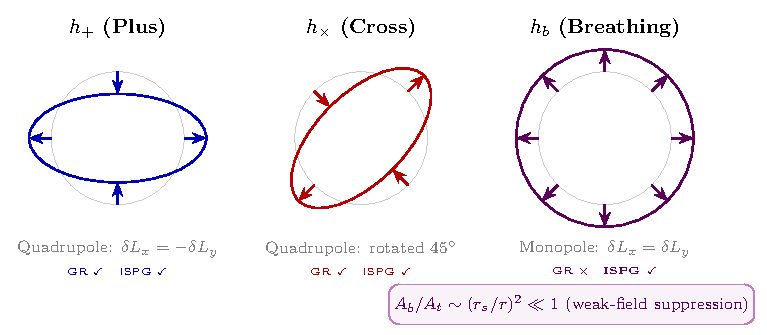
\includegraphics[width=0.75\textwidth]{PDF/fig_gw_polarizations.pdf}
\caption{Gravitational-wave polarization content.  The
tensor modes $h_{+}$ and $h_{\times}$ are shared with GR;
the breathing mode $h_{b}$ is absent in GR (and
distinctive relative to it; scalar breathing modes also
appear in other scalar--tensor theories) and is suppressed
at the source by an estimated $A_b/A_t\sim\rs/r$ in the
weak field (Eq.~\eqref{eq:breathing_ratio}; conditional on
the open scalar-quadrupole PN derivation in Appendix~10,
with leading-order $s=1/2$ from Appendix~16).
\label{fig:gw_pol}}
\end{figure}

%-------------------------------------------------------------------
\subsection{ISCO orbital-frequency proxy}\label{sec:merger}
%-------------------------------------------------------------------

The innermost stable circular orbit (derived in
Sec.~\ref{sec:singularity}) occurs at
$r_{\mathrm{ISCO}} = \phigr^{2}\,\rs \approx 2.618\,\rs$
in the isotropic coordinate of the bi-conformal metric,
compared to $r_{\mathrm{ISCO}}^{(\mathrm{GR,iso})}
\approx 2.47\,\rs$ in GR (or $3\,\rs$ in Schwarzschild
coordinates; see Sec.~\ref{sec:singularity}).
The coordinate-invariant test-particle circular-orbit
angular frequency in the bi-conformal exterior is
\begin{equation}\label{eq:Omega_circ}
  \Omega^{2}(r)
  = \frac{c^{2}\,\rs\,e^{-2\rs/r}}
         {r^{2}\,(2r - \rs)}\,,
\end{equation}
so that, evaluating both sides at their respective
ISCO radii,
\begin{equation}\label{eq:merger_ratio}
  \frac{f_{\mathrm{ISCO}}^{(\mathrm{this\;work})}}
       {f_{\mathrm{ISCO}}^{(\mathrm{GR})}}
  \approx 0.931\,,
\end{equation}
i.e.\ the test-particle ISCO orbital-frequency proxy is
$\approx 6.9\%$ lower than the GR value for the same
total mass.  For a $30 + 30\,M_{\odot}$ binary, this
proxy gives $f_{\mathrm{GR}} \approx 73\;\mathrm{Hz}$,
$f_{\mathrm{this\;work}} \approx 68\;\mathrm{Hz}$.
A direct confrontation with LIGO--Virgo--KAGRA data
through waveform-template matching requires an ISPG
waveform model (inspiral--merger--ringdown for
comparable-mass binaries, with consistent radiation
reaction and ringdown/QNM structure) and a corresponding
parameter-estimation pipeline; the test-particle
ISCO-frequency proxy alone cannot be substituted for
that ISPG waveform, since the GR mass parameters used
in current pipelines are template-inferred.  Both the
ISPG waveform and the population-level test are flagged
as future work.

%-------------------------------------------------------------------
\subsection{Scalar dipole radiation from mixed binaries}
\label{sec:dipole}
%-------------------------------------------------------------------

In generic scalar-tensor theories, when two bodies have
different scalar sensitivities $s_{A} \neq s_{B}$, the
binary acquires a scalar dipole moment and the orbital
energy loss rate gains a $-1$PN correction:
\begin{equation}\label{eq:dipole_power}
  \dot{E}_{\mathrm{dipole}} = -\frac{G\,\mu\,M}{3\,r^{2}}\,
  (s_{A} - s_{B})^{2}\,v\,,
\end{equation}
where $\mu$ is the reduced mass, $M$ the total mass,
and $v$ the orbital velocity.  This emission is lower order
than the standard quadrupole $\dot{E} \propto v^{5}$,
so it would dominate the early inspiral at large separation.
The resulting phase shift relative to the GR waveform
would accumulate as
\begin{equation}\label{eq:dipole_phase}
  \Delta\Psi_{\mathrm{dipole}} \sim
  \frac{5}{672}\,(s_{A}-s_{B})^{2}\,
  \left(\frac{GM\pi f}{c^{3}}\right)^{-7/3}\,.
\end{equation}

In the bi-conformal theory, the bare-mass Komar
integrand $\rho_0\,e^{-\phi}
= \rho_0\,e^{\phi/2}\,e^{-3\phi/2}$ (combining the
universal conformal redshift $e^{\phi/2}$ with the
proper-volume factor $e^{-3\phi/2}$; the redshift factor
alone, $m_{\mathrm{eff}} = m_0\,e^{\phi/2}$, is one
ingredient, not the whole derivation) selects
$s = 1/2$ at leading order in $|\phi|$ for every
body---test particles, white dwarfs, neutron stars, and
vacuum compact objects alike (Appendix~16,
Sec.~``Kinematic motivation'').  For vacuum compact
objects this result is \emph{exact}, derived from the
vacuum exterior harmonic monopole profile combined with the
rigid-shift response of the bare-mass Komar integral
(Appendix~16, Sec.~``No-hair property: scope'',
item~1).  For matter-filled bodies, the
exact cancellation of the residual structural-response
correction is an open task (Appendix~16, Sec.~``Shift
invariance: sectoral analysis'').  At leading order,
$(s_{A} - s_{B})^{2} \simeq 0$ for any binary, so the
scalar dipole channel is strongly suppressed.

\textit{Orbital-period derivative.}---The dipole
contribution to the period derivative is parametrically
\begin{equation}\label{eq:Pdot_dipole}
  \dot{P}_{b}^{(\mathrm{dipole})} \propto
  (s_{A} - s_{B})^{2} \simeq 0\,,
\end{equation}
where the dimensional prefactor follows the standard
scalar--tensor form (e.g.\ $\propto G(m_{1}+m_{2})/(c^{3}P_{b})$;
see Appendix~16, Eq.~\ref{eq:Pdot_dipole_app16}, and the
scalar-tensor literature for the full coefficient).  At
leading order $(s_{A}-s_{B})^{2}\simeq 0$, so the orbital
decay is purely quadrupolar at this order, as in GR.  This is qualitatively
consistent with the observed agreement of $\dot{P}_{b}$ with the GR
prediction at the $\sim 10\%$ level for
PSR~J1738+0333~\cite{Freire2012} (read as an
\emph{illustrative} bound, pending the ISPG-specific
$\kappa_D$ normalization that maps
$s_{\mathrm{excess}}$ to the standard pulsar dipole
coefficient; see Appendix~16
Sec.~``Compatibility-table footnote''), and with the
universality-of-free-fall bound from the triple system
PSR~J0337+1715~\cite{Archibald2018} (conservative 2018
value; tightened to model-dependent
$|\Delta|\lesssim 1.5$--$2.3\times10^{-6}$ by the 2025
Voisin et~al.\ re-analysis~\cite{Voisin2025}).

The structural reason is partially unique to the
bi-conformal framework, with the explicit status
recorded in Appendix~16: the interior hydrostatic
sub-equation depends only on $d\varphi/dr$ and is
\emph{exactly} rigid-shift invariant, whereas the
coupled scalar equation in matter carries an explicit
$e^{-\varphi}$ source factor and is only
\emph{leading-order} shift invariant in matter (exact
for vacuum compact objects via $\nabla^{2}\varphi=0$).
At leading order this is enough for $s_{A}\simeq s_{B}
\simeq 1/2$ and $(s_{A}-s_{B})^{2}\simeq 0$, distinguishing
the present theory from Brans--Dicke, DEF, and other
scalar-tensor theories that generically predict
$(s_{A}-s_{B})^{2}\neq 0$; the exact non-perturbative
matter-filled cancellation remains an open task
(Appendix~16, Sec.~``Shift invariance: sectoral
analysis'').

%===================================================================
\section{Phantom kinetic term and stability}\label{sec:phantom}
%===================================================================

The kinetic term in~(\ref{eq:action}) carries the phantom
sign ($+\half$ rather than $-\half$).  Standard concerns
about phantom fields include Hamiltonian unboundedness,
vacuum instability via ghost--tensor pair production,
and ill-posedness of the Cauchy
problem~\cite{Carroll2003,Cline2004,Sbisa2015}.
Below we show that, in the present context, none of
these pathologies arise.

%-------------------------------------------------------------------
\subsection{Hyperbolicity and well-posedness}
\label{sec:hyperbolicity}
%-------------------------------------------------------------------

The linearized field equations for perturbations
$(h_{\mu\nu},\delta\varphi)$ about a background
$(\bar{g}_{\mu\nu},\bar{\varphi})$, after a standard
gauge-fixing/reduced formulation (e.g.\ harmonic or de Donder
gauge), have the principal symbol
\begin{equation}\label{eq:principal}
  \mathcal{P}(\xi) =
  \begin{pmatrix}
    \bar{g}^{\alpha\beta}\xi_{\alpha}\xi_{\beta}\,
    \mathbb{I}_{\mathrm{tensor}} & 0 \\
    0 & \bar{g}^{\alpha\beta}\xi_{\alpha}\xi_{\beta}
  \end{pmatrix},
\end{equation}
where $\xi_{\mu}$ is the perturbation covector.  Without such
a gauge fixing, the raw Einstein equations carry a
diffeomorphism-degenerate principal symbol and~\eqref{eq:principal}
should be read as the gauge-reduced form.  The characteristic
surfaces are determined by
$\bar{g}^{\alpha\beta}\xi_{\alpha}\xi_{\beta} = 0$,
which defines the null cone of the background metric.
Since $\bar{g}_{\mu\nu}$ has Lorentzian signature, the
characteristic equation has real roots for all spatial
wave directions; in the standard gauge-fixed/first-order
formulation the system is \emph{strongly hyperbolic}
and the Cauchy problem is well-posed in Sobolev
spaces~\cite{Papallo2018,Kovacs2020} (the symmetrizer and
eigenvector-completeness statements that elevate ``real
characteristic roots'' to ``strong hyperbolicity'' are those
of the cited literature).

All propagating modes---tensor and scalar---travel at
exactly $c$ in the local frame.  The tensor channel is
directly constrained by GW170817~\cite{LIGO_GW170817}
($c_g = c$ within a few$\times 10^{-15}$);
scalar luminality follows internally from the
principal-symbol/strong-hyperbolicity analysis above and
is not a separate experimental claim.  There is no
superluminal propagation and no violation of causality.

%-------------------------------------------------------------------
\subsection{Classical mode stability}
\label{sec:mode_stability}
%-------------------------------------------------------------------

\textit{Static background.}---Around the spherically
symmetric solution $\varphi = -\rs/r$, scalar perturbations
decomposed in spherical harmonics
$\delta\varphi = \sum_{\ell m}u_{\ell}(r)\,Y_{\ell m}/r$
satisfy a Schr\"odinger-type radial equation with an
effective potential
\begin{equation}\label{eq:Veff_pert}
  V_{\mathrm{eff}}(r) = e^{-2\rs/r}\left[
    \frac{\ell(\ell+1)}{r^{2}}
    + \frac{\rs}{r^{3}} - \frac{\rs^{2}}{4r^{4}}
  \right].
\end{equation}
For $\ell \geq 1$ the centrifugal barrier dominates
the bracket in the exterior; in the deep interior the
bracket can change sign, but the exponential prefactor
$e^{-2\rs/r}$ suppresses the resulting well far more
effectively than in the $\ell=0$ case, yielding a
Bargmann integral $\mathcal{I}\lesssim 10^{-7}$.
No bound state exists for any $\ell$.

For $\ell=0$ the potential $V_{\mathrm{eff}}^{(\ell=0)}$ is negative
in the interval $0<r<\rs/4$, but this well is exponentially
suppressed by the factor $e^{-2\rs/r}$.  Numerically, the
well integral
$\mathcal{I}=\int_{\mathrm{well}}|V_{\mathrm{eff}}|\,dr_*
\approx 1.0\times 10^{-4}$
(in units $c=\rs=1$).
By the Bargmann bound, a one-dimensional potential well supports
no bound state when $\mathcal{I}\ll 1$.  Therefore, no tachyonic
mode ($\omega^2<0$) exists at probe level even for $\ell=0$.
The full symbolic and numerical verification is given in Appendix~15.

\textit{Cosmological background.}---On the FLRW background
(Sec.~\ref{sec:cmb}), inhomogeneous scalar perturbations
satisfy
\begin{equation}\label{eq:pert_cosmo_stab}
  \ddot{\delta\varphi}_{k} + 3H\,\dot{\delta\varphi}_{k}
  + \frac{k^{2}c^{2}}{a^{2}}\,\delta\varphi_{k} = 0\,,
\end{equation}
with $\omega_{k}^{2} = k^{2}c^{2}/a^{2} > 0$.  All modes
oscillate and are damped by Hubble friction; there is no
gradient instability.

%-------------------------------------------------------------------
\subsection{Ghost elimination via constraint structure}
\label{sec:ghost}
%-------------------------------------------------------------------

In the unconstrained (effective field theory) formulation
the theory has $2 + 1 = 3$ degrees of freedom (two tensor,
one scalar), and the phantom scalar carries negative
kinetic energy in the Hamiltonian.  In a generic theory
this would trigger vacuum decay via ghost--tensor pair
production at a rate set by the UV cutoff.

The bi-conformal metric
structure~(\ref{eq:metric}) determines the \emph{entire}
background metric from the single function $\varphi$,
reducing the physical gravitational degrees of freedom to
\textbf{one} on the background.  A single phantom field
cannot decay into itself within the pure-gravity sector;
vacuum pair production requires a second field with
compensating positive energy, which is absent among
the gravitational modes of the constrained sector.
A matter-mediated channel
$|0\rangle\to|\varphi_{-E}\rangle+|\psi\bar\psi\rangle_{+E}$
with minimally coupled matter $\psi$ as positive-energy
partner remains kinematically open; its physical rate is
controlled by gravitational coupling strength (see
Appendix~11, ``Scope of the theorem'') and is
Planck-suppressed at all astrophysically relevant energies,
with the $\alpha X^{2}/M^{2}$ EFT completion
(Eq.~\ref{eq:ghost_condensation}) providing the UV
closure for this channel.

\textit{Scope.}---The 1-DOF reduction applies strictly to
the bi-conformal background, which is isotropic by
construction.  General perturbations (including
gravitational waves) break this isotropy and propagate in
the unconstrained 3-DOF sector.  Their classical stability
is guaranteed by the hyperbolicity established in
Sec.~\ref{sec:hyperbolicity}: the phantom sign does not affect
the principal symbol, so all modes have real characteristics
and well-posed Cauchy evolution.  The quantum extension
of the theory~\cite{Lotishvili2026Q} confirms that
pair-production rates are Planck-suppressed: loop
corrections scale as $(E/\Mpl)^{2} \sim 10^{-76}$,
the reduced Hamiltonian constraint algebra is argued to be
Abelian and anomaly-free at the level of the structural
analysis of~\cite{Lotishvili2026Q} (\emph{reduced} denotes
the gauge-fixed single-DOF phase space, distinct from the
full Dirac--Bergmann phase space of Appendix~11, whose
$(\Phi_\alpha,\bar\Phi_\alpha)$ conditions are second-class by
construction; a fully rigorous bracket-closure proof is
left as future work), and the Hamiltonian is bounded from
below non-perturbatively within the pure-gravity constrained
sector (the matter-coupled extension is controlled by the
EFT completion described below, not by this constraint
argument alone).
Quantum vacuum decay is therefore negligible at all
astrophysically relevant energies.

A complementary low-energy EFT phrasing is available even
without invoking the full quantum completion.  Away from the
strict bi-conformal background one may extend the minimal
Horndeski kinetic function to
\begin{equation}\label{eq:ghost_condensation}
  G_{2}(X) = -\frac{\Mpl^{2}}{2}\,X
    + \frac{\alpha}{M^{2}}\,X^{2}\,,
    \qquad \alpha > 0\,,
\end{equation}
with $X \equiv -\half\,g^{\mu\nu}\partial_{\mu}\varphi\,
\partial_{\nu}\varphi$.  The condensate then sits at nonzero
$\langle X\rangle$ where $\partial G_{2}/\partial X > 0$,
stabilizing the kinetic sector while leaving the weak-field
static solution unchanged at the order relevant for Solar-system
and 2PN observables~\cite{ArkaniHamed2004}.  The exponential
bi-conformal metric, the ensuing structurally distinct 2PN
Shapiro signature (Sec.~\ref{sec:shapiro}), and the ISCO radius
are therefore infrared predictions rather than artifacts of a
particular UV completion.

This distinction is critical because Bronnikov and
collaborators~\cite{Bronnikov2012} have shown that
phantom-scalar wormholes are linearly unstable under
spherically symmetric perturbations in the
\emph{unconstrained} formulation---the instability is
catastrophic, with perturbation growth rates that are
unbounded from above.  The constrained (fundamental)
formulation eliminates the unstable mode by construction.

A further structural distinction separates the present
solution from the Bronnikov wormholes: the bi-conformal
background~(\ref{eq:metric_static}) has only one physically
accessible exterior (the $r \to \infty$ side).  The areal
radius $R(r) = r\,e^{\rs/(2r)}$ does have a coordinate-level
minimum at $r = \rs/2$ and the $r \to 0^{+}$ side admits a
formal asymptotic limit (Appendix~12), but that side is
causally inert in the present analysis: no traversable
throat connects two physically realized asymptotic regions.
The Bronnikov--Rubin instability arises from a mode that
threads such a throat, coupling two physical exteriors; in
the absence of a second realized exterior this mode has no
support.  This effective one-sided causal topology, combined
with the exponential suppression
$e^{-2\rs/r}$ in the deep interior, restricts perturbation
dynamics to a regime where the Bargmann analysis
(Appendix~15) already excludes tachyonic modes.  Task~1b
(even/polar sector) remains the definitive test, but the
topological mismatch gives strong reason to expect that
the Bronnikov instability does not carry over.

The closest precedents in the literature are
\emph{cuscuton gravity}~\cite{Afshordi2007}, where
$\nabla_{\!\mu}\varphi\,\nabla^{\mu}\varphi = \mu^{2}$
eliminates the scalar propagator, and
\emph{mimetic gravity}~\cite{Chamseddine2013}, where a
conformal constraint does likewise.  In all three cases
the ghost is removed kinematically by the constraint,
not dynamically stabilized.

The formal Dirac--Bergmann analysis is carried out in
Appendix~11.  The bi-conformal conditions are exhibited
as second-class constraints in the ADM phase space,
reducing the physical degrees of freedom from three
(two tensor $+$ one scalar) to \textbf{one}.  A single
propagating DOF has no pair-production channel: the
process $|0\rangle\to|\text{ghost}\rangle+|\text{tensor}\rangle$
requires at least two independent fields, and the
constrained formulation provides only one.  The energy
of the remaining DOF need not be positive-definite---the
phantom sign is intrinsic---but no runaway occurs because
there is no decay partner.  The full DOF count, stability
theorem, and relation to cuscuton and mimetic gravity
are given in Appendix~11.

%-------------------------------------------------------------------
\subsection{Energy conditions}\label{sec:energy_conditions}
%-------------------------------------------------------------------

The scalar energy-momentum tensor~(\ref{eq:Tphi}) as
defined is canonical and in fact \emph{satisfies} the
standard energy conditions:  for a null vector $k^{\mu}$,
\begin{equation}\label{eq:nec}
  \tau_{\mu\nu}^{(\varphi)}\,k^{\mu}k^{\nu}
  = (k^{\mu}\partial_{\mu}\varphi)^{2} \geq 0\,,
\end{equation}
and analogous non-negativity holds for a timelike
$u^{\mu}$ after accounting for the phantom kinetic sign
(the WEC/SEC analogues follow by the same canonical-tensor
algebra used in~\eqref{eq:nec}).  What violates the
energy conditions is the \emph{effective source} that
enters the Einstein equation~(\ref{eq:einstein}): the
coupling factor $\kappa = -\frac12$ flips the sign of the
scalar contribution, so the effective NEC quantity is
\begin{equation}\label{eq:nec_effective}
  \kappa\,\tau_{\mu\nu}^{(\varphi)}\,k^{\mu}k^{\nu}
  = -\tfrac{1}{2}(k^{\mu}\partial_{\mu}\varphi)^{2}\leq 0\,,
\end{equation}
and likewise for WEC and SEC.  Thus the phantom sign
makes the effective gravitational source violate the
energy conditions, while the canonical tensor
$\tau_{\mu\nu}^{(\varphi)}$ itself does not.  The violation is
an intrinsic property of how $\varphi$ couples to geometry
through $\kappa$, not of the tensor form in~(\ref{eq:Tphi}).

The effective NEC violation has a direct physical
consequence:
it invalidates the focusing theorem that underpins the
Penrose--Hawking singularity
theorems~\cite{Penrose1965,Hawking1970}.  This is what
allows the singularity resolution derived in
Sec.~\ref{sec:singularity}---the same mechanism that
makes the phantom sign troublesome in flat-space QFT
is precisely what cures the classical singularity.

%-------------------------------------------------------------------
\subsection{Absence of a fifth force}\label{sec:fifth_force}
%-------------------------------------------------------------------

In generic scalar--tensor theories a light scalar field
mediates a fifth force constrained by torsion-balance
experiments~\cite{Adelberger2003}.
The present theory evades these bounds for three reasons:
(i)~matter is minimally coupled to the single physical
metric~(\ref{eq:metric}), so the test-particle weak
equivalence principle is satisfied identically
($\eta_{\mathrm{E\ddot{o}t}} < 10^{-15}$);
(ii)~the weak-field limit yields
$\gamma_{\mathrm{PPN}} = \beta_{\mathrm{PPN}} = 1$
(Sec.~\ref{sec:ppn}), making the scalar indistinguishable
from GR at first post-Newtonian order;
(iii)~the first observable deviation appears at the
\emph{second} post-Newtonian level
(Sec.~\ref{sec:shapiro}), which is below the sensitivity
of current laboratory and Solar-system tests.
Consequently, the scalar sector is not a ``fifth force''
in the experimental sense; it is an integral part of
gravity, distinguishable only in the strong-field or
high-precision regime.

%===================================================================
\section{Singularity resolution and compact objects}
\label{sec:singularity}
%===================================================================

%-------------------------------------------------------------------
\subsection{Curvature regularity}\label{sec:curvature}
%-------------------------------------------------------------------

The exact bi-conformal metric~(\ref{eq:metric_static}) with
$\varphi = -\rs/r$ yields the Ricci and Kretschmann scalars
(verified symbolically with
\texttt{MAIN/Python/Shapiro/check\_ricci\_kretschmann.py}, which checks
the full closed form of Eq.~(\ref{eq:kretschner}) against
the SymPy-computed curvature and additionally reports the
Schwarzschild leading term for comparison):
\begin{align}
  R &= -\frac{\rs^{2}}{2r^{4}}\,e^{-\rs/r}\,,
  \label{eq:ricci}\\[4pt]
  K \equiv R_{\mu\nu\rho\sigma}R^{\mu\nu\rho\sigma}
    &= \frac{\rs^{2}}{4r^{8}}\Bigl(48r^{2}-32r\,\rs+7\rs^{2}\Bigr)\,
       e^{-2\rs/r}\,.
  \label{eq:kretschner}
\end{align}
In the weak-field regime $\rs/r\ll 1$ this expands as
$K = \bigl(12\,\rs^{2}/r^{6}+O(\rs^{3}/r^{7})\bigr)e^{-2\rs/r}$,
recovering the Schwarzschild leading term.
As $r \to 0$ the exponential factor $e^{-\rs/r}$ (respectively
$e^{-2\rs/r}$) vanishes faster than any power of $1/r$
diverges.  Consequently, the displayed curvature invariants
vanish at the origin:
\begin{equation}\label{eq:K_limit}
  \lim_{r\to 0} R = 0\,,\qquad
  \lim_{r\to 0} K = 0\,.
\end{equation}
The Kretschmann scalar reaches a finite maximum at
$r \approx 0.221\,\rs$
(equivalently $u\equiv\rs/r\approx 4.524$, the unique real root of
$7u^{3}-60u^{2}+160u-144=0$ on the physical domain):
\begin{equation}\label{eq:K_max}
  K_{\max} \approx \frac{11.72}{\rs^{4}}\,.
\end{equation}
For astrophysical black holes this is far below the
Planck curvature $K_{\mathrm{Pl}} = \ell_{P}^{-4}$.

\paragraph{$r=0$ is not a regular centre: global structure.}
The vanishing of curvature invariants at $r=0$ should not
be read as collapse to a regular origin.  The areal radius
of a sphere of coordinate radius $r$ in the bi-conformal
metric~(\ref{eq:metric_static}) is
\begin{equation}\label{eq:areal}
  R(r) \equiv r\,e^{\rs/(2r)}\,,
\end{equation}
which has a minimum at the coordinate-level throat
$r=\rs/2$, $R_{\min} = (\rs/2)\,e \approx 1.36\,\rs$, and
grows without bound in \emph{both} limits $r\to\infty$ (the
usual physical exterior) and $r\to 0^{+}$ (a formal/deep-interior
asymptotic region, causally inert and unobservable from the
exterior in the present analysis; cf.\ the Bronnikov-distinction
discussion above).  The coordinate $r=0$ is therefore not a
point at finite proper distance but a formal asymptotic limit
of the deep interior.  The areal-radius geometry, the
coordinate throat, and the question of whether the second
asymptotic limit is ever physically realisable are developed
in Appendix~12 (Sec.~``Wormhole structure''); the present
section restricts itself to the curvature-invariant statement.

\begin{figure}[t]
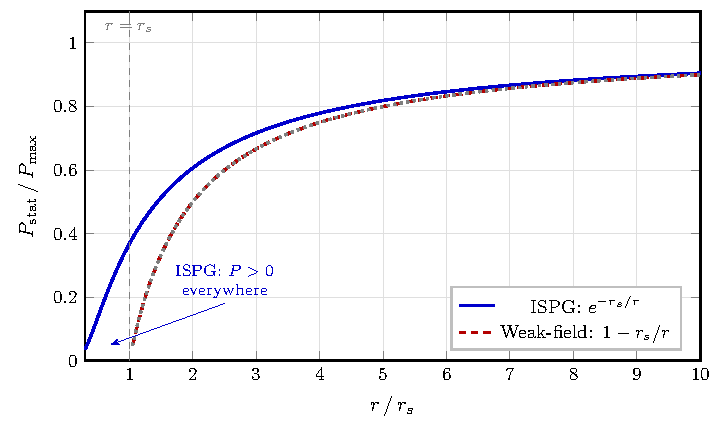
\includegraphics[width=0.75\textwidth]{PDF/fig_pressure_profile.pdf}
\caption{Normalised IS pressure $P_{\mathrm{stat}}/P_{\max}$
versus radial coordinate.  The solid curve shows the exact
exponential profile; the dashed curve is the weak-field
expansion truncated at second order.  The two diverge
below $r \approx 2\,\rs$, illustrating how the full
nonlinear solution avoids the singularity present in any
finite-order expansion.
\label{fig:pressure_profile}}
\end{figure}

\begin{figure}[t]
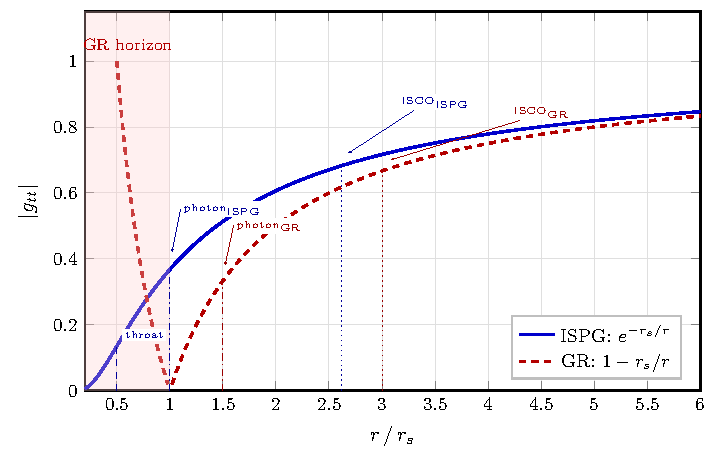
\includegraphics[width=0.75\textwidth]{PDF/fig_gtt_comparison.pdf}
\caption{Absolute value of the metric component $g_{tt}$
as a function of $r/\rs$.  In GR (dashed), $g_{tt}$
vanishes at the horizon $r = \rs$; in the present theory
(solid), $g_{tt} = e^{-\rs/r}$ is strictly nonzero.
Vertical markers indicate the throat of the wormhole
geometry at $r=\rs/2$ (see Eq.~(\ref{eq:areal}) and
Appendix~12), photon spheres, and ISCOs for both theories.
\label{fig:gtt}}
\end{figure}

%-------------------------------------------------------------------
\subsection{Geodesic completeness}\label{sec:geodesic}
%-------------------------------------------------------------------

The proper radial distance from any radius $r_{0}$ to
the origin is
\begin{equation}\label{eq:proper}
  \ell_{\rm prop} = \int_{0}^{r_{0}}\!\sqrt{g_{rr}}\,dr
    = \int_{0}^{r_{0}}\!e^{\,\rs/(2r)}\,dr\,.
\end{equation}
As $r \to 0$ the integrand $e^{\rs/(2r)}$ diverges
exponentially, and the integral diverges:
$\ell_{\rm prop} \to \infty$.  The center $r = 0$ is at \emph{infinite
proper distance}.  Radial geodesics nonetheless reach
$r = 0$ in finite proper time (or affine parameter),
since $\dot{r}^{2}\to E^{2}/c^{2}>0$ as $r\to 0$.
The Appendix~12 effective potential
$V_{\mathrm{eff}}(r)=\kappa c^{2}e^{-\rs/r}
+\mathcal{L}^{2}e^{-2\rs/r}/r^{2}$
peaks at the photon sphere ($r = \rs$) and is
exponentially suppressed to zero as $r \to 0$
(Appendix~12; cf.\ Fig.~\ref{fig:Veff}).
Geodesics that do not cross this barrier
(impact parameter $b > b_{c} = \rs\,e$) are
reflected and complete; those that cross it
reach $r = 0$ in finite proper time, making the
spacetime geodesically incomplete.

\paragraph{Scope of the ``singularity-free'' claim.}
In the Hawking--Penrose convention, geodesic
incompleteness is itself a definition of
singularity, so the present geometry is not
globally non-singular.  What we \emph{do} show is
the following restricted set of statements:
(i)~every polynomial curvature invariant is
finite---indeed vanishes---at $r = 0$
(Sec.~\ref{sec:curvature}); (ii)~the boundary is
at infinite proper distance and carries infinite
redshift ($1+z = e^{\rs/(2r)} \to \infty$);
(iii)~it requires infinite coordinate time to
reach, so it is causally inert and unobservable
from the exterior; (iv)~tidal forces decrease
monotonically toward zero on approach.  By
contrast, the Schwarzschild singularity fails
(i)~and~(iv).  Whether the $r = 0$ boundary admits
a low-regularity metric extension, and whether any
such extension can be made smooth and satisfy the
field equations, remains open.  Bounded displayed
curvature invariants motivate the extension question,
but they do not by themselves satisfy the hypotheses
of a Clarke-type extension theorem (Appendix~12,
Sec.~``Classification of the $r=0$ boundary'').
Accordingly, ``singularity-free'' in this paper
refers to (i)--(iv) and not to the Hawking--Penrose
completeness criterion.

\begin{figure}[t]
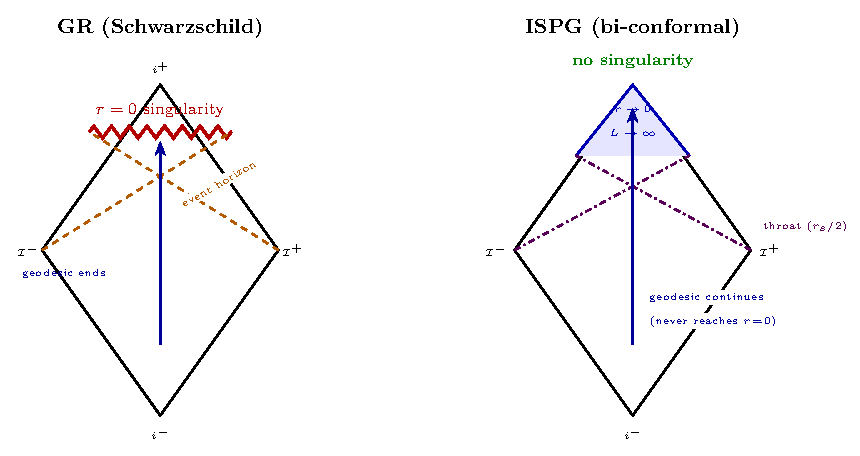
\includegraphics[width=0.75\textwidth]{PDF/fig_penrose.pdf}
\caption{Penrose (conformal) diagrams.  \textit{Left:}
Schwarzschild spacetime---the curvature singularity at
$r = 0$ destroys infalling matter.  \textit{Right:}
Bi-conformal spacetime---$r = 0$ is at infinite proper
distance with vanishing curvature; the boundary is
curvature-regular, at infinite redshift, and causally
inert from the exterior, but geodesically incomplete
(Appendix~12).  The throat
at $\rs/2$ connects the exterior to the deep interior.
\label{fig:penrose}}
\end{figure}

%-------------------------------------------------------------------
\subsection{Horizonless compact object}\label{sec:horizonless}
%-------------------------------------------------------------------

The metric component $g_{tt}=-e^{-\rs/r}$ is nonzero
for every manifold point $r>0$, so the static exterior has
no finite-radius Killing horizon.  Radial outgoing null rays obey
$dr/dt=c\,e^{-\rs/r}>0$ for every $r>0$, and therefore can move
outward from any finite radius.  This establishes the horizonless
statement used here in the finite-radius static exterior sense; a
fully global event-horizon statement would require a collapse
spacetime and a boundary condition at $r=0$, which are not
constructed in this paper.  Instead, the areal radius
$R(r) = r\,e^{\rs/(2r)}$ has a minimum at
\begin{equation}\label{eq:throat}
  r_{\mathrm{throat}} = \frac{\rs}{2}\,,
\end{equation}
where $dR/dr = 0$.  This is a throat (minimum-area surface),
not a horizon:
\begin{itemize}
\item $g_{tt}(\rs/2) = -e^{-2} \approx -0.135$ (nonzero);
\item an outgoing photon emitted at any finite $r>0$ reaches
  any finite exterior radius in finite coordinate time, and
  encounters no finite-radius horizon on its way to future
  null infinity;
\item the structure is a one-sided wormhole throat with
  infinite depth ($\ell_{\rm prop} \to \infty$).
\end{itemize}

Current ringdown and echo searches do not yet provide a decisive
horizon test; GWTC-3 tests remain consistent with GR and find no
confirmed post-merger echoes~\cite{Cardoso2019,Miani2023,LVK2025TGR}.
The same qualitative picture
is also consonant with Gogberashvili's arguments that quantum
particles are reflected at the Schwarzschild horizon and that
smooth interior--exterior matching requires the source radius
to lie outside the photon sphere~\cite{Gogberashvili2018,Gogberashvili2019}.

%-------------------------------------------------------------------
\subsection{Innermost stable circular orbit}\label{sec:isco}
%-------------------------------------------------------------------

The effective potential for massive test particles on
equatorial geodesics is
\begin{equation}\label{eq:Veff}
  V_{\mathrm{eff}}(r) = e^{\varphi}\!\left(
    1 + \frac{\mathcal{L}^{2}\,e^{\varphi}}{r^{2}}\right),
  \qquad \varphi = -\frac{\rs}{r}\,.
\end{equation}
Circular orbits require $V_{\mathrm{eff}}'= 0$; stability
requires $V_{\mathrm{eff}}'' \geq 0$.  The ISCO condition
$V_{\mathrm{eff}}'' = 0$ reduces to the algebraic equation
\begin{equation}\label{eq:isco_eq}
  r^{2} - 3\,\rs\,r + \rs^{2} = 0\,,
\end{equation}
with the physical solution
\begin{equation}\label{eq:isco}
  \boxed{r_{\mathrm{ISCO}}
    = \frac{3+\sqrt{5}}{2}\,\rs
    = \phigr^{2}\,\rs
    \approx 2.618\,\rs\,,}
\end{equation}
where $\phigr = (1+\sqrt{5})/2$ is the golden ratio.
The appearance of $\phigr^{2}$ is not imposed---it
emerges from the quadratic~(\ref{eq:isco_eq}), whose
coefficients $(1,-3,1)$ are dictated by the exponential
metric.  It was unexpected, and the author verified it
independently with SageManifolds before accepting
the result.  In Schwarzschild coordinates, the GR ISCO
is at $6\,GM/c^{2} = 3\,\rs$; converting to isotropic
coordinates gives
$r_{\mathrm{ISCO}}^{(\mathrm{GR,iso})} =
\tfrac{1}{4}(5+2\sqrt{6})\,\rs \approx 2.47\,\rs$.
The present value ($2.618\,\rs$) is $5.8\%$ farther
in consistent isotropic coordinates.  The physically
unambiguous comparison is the test-particle ISCO
orbital-frequency proxy, which is $6.9\%$ lower than
in GR (Sec.~\ref{sec:merger}).

\begin{figure}[t]
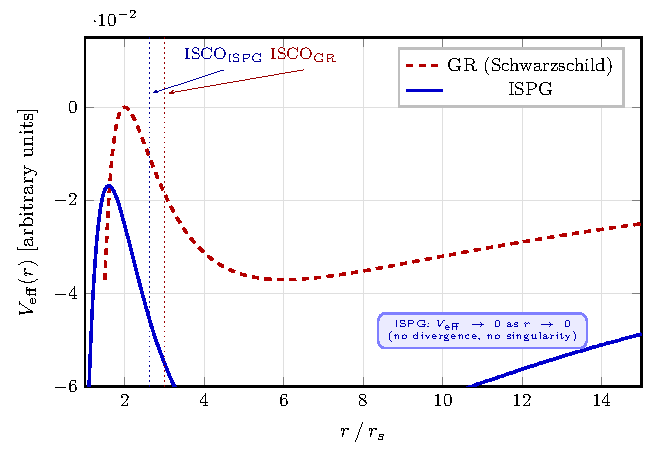
\includegraphics[width=0.75\textwidth]{PDF/fig_effective_potential.pdf}
\caption{Effective potential for massive test particles.
In GR (dashed) $V_{\mathrm{eff}}$ diverges as
$r \to 0$; in the present theory (solid) the exponential
suppression drives $V_{\mathrm{eff}} \to 0$.  The ISCO
locations are marked: $\phigr^{2}\,\rs \approx 2.618\,\rs$
(this work, isotropic coordinate) versus $3\,\rs$ (GR,
Schwarzschild coordinate; $\approx 2.47\,\rs$ in
isotropic coordinates).
\label{fig:Veff}}
\end{figure}

%-------------------------------------------------------------------
\subsection{Photon sphere}\label{sec:photon_sphere}
%-------------------------------------------------------------------

Null circular orbits satisfy
$\frac{d}{dr}(e^{2\varphi}/r^{2}) = 0$, giving
\begin{equation}\label{eq:photon}
  r_{\mathrm{photon}} = \rs\,.
\end{equation}
In Schwarzschild spacetime the photon sphere is at
$r^{(\mathrm{GR})} = 3\,GM/c^{2} = \frac{3}{2}\,\rs$
(Schwarzschild coordinate); in isotropic coordinates
this maps to $r^{(\mathrm{GR,iso})} =
\tfrac{1}{4}(2+\sqrt{3})\,\rs \approx 0.933\,\rs$.
The present value ($\rs$) is $7.2\%$ farther in
consistent isotropic coordinates.  A chart-invariant
comparison is the critical impact parameter (shadow size):
$b_{c} = \rs\,e \approx 2.718\,\rs$ versus
$b_{c}^{(\mathrm{GR})} = \tfrac{3\sqrt{3}}{2}\,\rs
\approx 2.598\,\rs$, a $4.6\%$ larger shadow.  The
invariance is conditional on the asymptotic Killing-vector
normalization (Minkowski-asymptotic $g_{tt}\to-1$ and
$2\pi$-period $\partial_\phi$), which is shared between the
bi-conformal and Schwarzschild charts; under this shared
normalization the comparison is direct, without the
coordinate-translation issue that affects the ISCO radius.
This prediction is \emph{consistent} with current Event
Horizon Telescope observations of M87\textsuperscript{*}
(shadow diameter $42\pm 3\,\mu$as, $\sim 7\%$ systematic
uncertainty)~\cite{EHT2019M87,EHT2024M87} and
Sgr~A\textsuperscript{*} ($51.8\pm 2.3\,\mu$as,
$\sim 4.4\%$ statistical)~\cite{EHT2022}, within which ISPG
and GR are not yet observationally distinguishable; the
predicted $4.6\%$ difference is comparable to current
ring-measurement uncertainties, and translation between the
geometric-optics critical curve $b_c$ and the observed
emission-ring diameter further depends on mass and distance
priors, spin, inclination, and accretion-emission modelling.
A \emph{decisive} test awaits future shadow-related
measurements at the few-percent or better level, with
constrained imaging models, in the next-generation EHT
regime.  Epistemic status: prediction derived from the
theory under the static spherical vacuum assumption; current
data compatible; decisive falsification deferred to future
instrumentation and rotating-extension modelling.

%-------------------------------------------------------------------
\subsection{Summary of compact-object predictions}
\label{sec:compact_summary}
%-------------------------------------------------------------------

\begin{table}[ht]
\caption{Compact object: comparison with Schwarzschild.
\label{tab:compact}}
\begin{ruledtabular}
\begin{tabular}{lcc}
Property & This work & GR (Schwarzschild) \\
\hline
Singularity at $r=0$ & No ($K\to 0$) & Yes ($K\to\infty$) \\
Geodesic completeness & No$^{\ddagger}$ & No \\
Finite-radius Killing horizon & None & $r = \rs$ \\
ISCO (isotropic coord., this work) & $\phigr^{2}\,\rs \approx 2.618\,\rs$ & $3\,\rs$ (Schw.) / $\approx 2.47\,\rs$ (iso.) \\
Photon sphere & $\rs$ & $\frac{3}{2}\,\rs$ (Schw.) \\
ISCO orbital-frequency proxy & $-6.9\%$ vs GR & Reference \\
\end{tabular}
\end{ruledtabular}
\smallskip\noindent{\footnotesize $^{\ddagger}$Geodesics
that cross the photon-sphere barrier ($b < \rs\,e$) reach
$r = 0$ in finite proper time; the boundary is
curvature-regular ($K\to0$), at infinite redshift, and
unobservable from outside (Appendix~12).}
\end{table}

\begin{figure}[t]
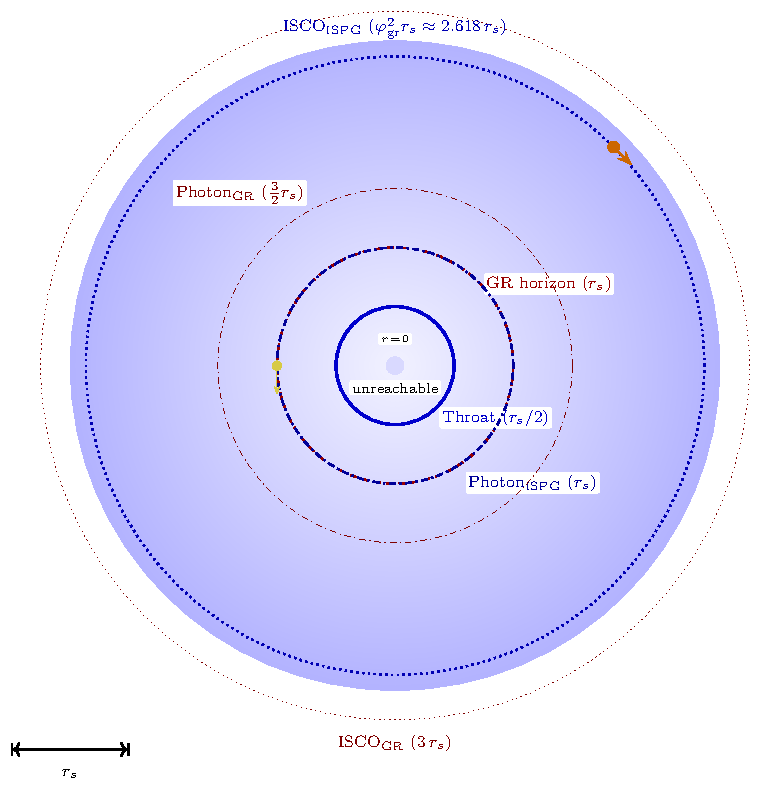
\includegraphics[width=0.75\textwidth]{PDF/fig_compact_object.pdf}
\caption{Schematic radial structure of the bi-conformal compact
object.  In GR (outer labels) the event horizon lies at $\rs$;
in the present theory (inner labels) $\rs$ is the photon sphere,
$\rs/2$ is the throat (minimum areal radius), and the ISCO
occurs at $\phigr^{2}\,\rs \approx 2.618\,\rs$.  The center
$r = 0$ is at infinite proper distance and regular in the
displayed polynomial invariants ($R, K \to 0$).
\label{fig:compact_object}}
\end{figure}

%===================================================================
\section{Cosmological perturbations and CMB compatibility}
\label{sec:cmb}
%===================================================================

%-------------------------------------------------------------------
\subsection{FLRW background}\label{sec:flrw}
%-------------------------------------------------------------------

On the Friedmann--Lema\^{\i}tre--Robertson--Walker metric
$ds^{2} = -c^{2}\,dt^{2} + a^{2}(t)\,\delta_{ij}\,dx^{i}dx^{j}$,
the reduced homogeneous metric-sector branch uses a scalar
$\varphi_{0}(t)$ satisfying
\begin{equation}\label{eq:flrw_scalar}
  \ddot{\varphi}_{0} + 3H\,\dot{\varphi}_{0} = 0\,,
\end{equation}
with general solution $\dot{\varphi}_{0} = C_{0}/a^{3}$.
This equation is not used as an independent pressure-history
closure: matter-sourced scalar response is treated through
inhomogeneous perturbations and through the quasi-static
bound-structure sector, not as a second homogeneous FLRW
metric background.
The bi-conformal ansatz of Eq.~(\ref{eq:metric}) is the
static spherically-symmetric vacuum form, in which
$g_{tt} = -e^{\varphi}$.  On the FLRW background written
in the matter-clock cosmic-time gauge ($t = \tau$,
$g_{tt} = -1$), the \emph{same} temporal condition
fixes $e^{\varphi_{0}} = 1$, i.e.\ $\varphi_{0} = 0$
at all times, and hence $C_{0} = 0$.  This is a
\emph{consistency consequence of the construction} in
the cosmic-time gauge, not an independent dynamical
prediction (see Appendix~9, ``Clarifying remark'').
In non-comoving time parametrizations ($t \neq \tau$)
one may keep $\varphi_{0} \neq 0$, but then the
background is no longer written in the standard FLRW
cosmic-time gauge.  On the spatial side, the
bi-conformal ansatz $g_{ij} = e^{-\varphi}\delta_{ij}$
is the static isotropic form and is not imposed on the
cosmological metric; only the temporal matching is used
to fix the homogeneous scalar.

Given $\varphi_{0} = 0$ (hence $\dot{\varphi}_{0} = 0$),
the scalar field carries no homogeneous cosmological
energy density: the background cosmology reproduces
standard Friedmann,
\begin{equation}\label{eq:friedmann}
  3\Mpl^{2}\,H^{2} = \rho_{\mathrm{m}}\,,\qquad
  \rho_{\varphi} = 0\,.
\end{equation}
The alternative branch $C_{0} \neq 0$ gives
$\rho_{\varphi} = -C_{0}^{2}/(2a^{6})$, a phantom
transient decaying faster than any matter component; its
stability against ghost modes requires the EFT
completion of Appendix~11 (cf.\ Sec.~\ref{sec:phantom}).

%-------------------------------------------------------------------
\subsection{Bellini--Sawicki parameters}\label{sec:bellini}
%-------------------------------------------------------------------

The Bellini--Sawicki parameterization~\cite{BelliniSawicki2014}
characterizes linear perturbations in Horndeski theories through
four time-dependent functions.  For the Horndeski
map~(\ref{eq:horndeski_map}) with $\varphi_{0} = 0$:

\medskip\noindent
\textit{Planck mass.}---$M_{*}^{2} = 2G_{4} = \Mpl^{2}$
(constant).

\medskip\noindent
\textit{Running.}---$\alpha_{M} = d\ln M_{*}^{2}/d\ln a = 0$.

\medskip\noindent
\textit{Tensor speed.}---$\alpha_{T} = 0$
\;($G_{4,X} = G_{5} = 0$).

\medskip\noindent
\textit{Braiding.}---$\alpha_{B} = 0$
\;($G_{3} = 0$, $G_{4,\varphi} = 0$).

\medskip\noindent
\textit{Kineticity.}---The Horndeski map $G_{2} = -(\Mpl^{2}/2)\,X$
(consistent with~\eqref{eq:horndeski_map})
gives $\alpha_{K} = -\dot{\varphi}_{0}^{2}/(2H^{2})$.
On the background $\dot{\varphi}_{0} = 0$
(\S\ref{sec:flrw}), $\alpha_{K} = 0$ trivially.  For
$\dot{\varphi}_{0} \neq 0$ (e.g.\ the $C_{0} \neq 0$
transient of \S\ref{sec:flrw}), $\alpha_{K} < 0$ exposes
the phantom kinetic sign; the EFT completion of
Appendix~11 is assumed to stabilize such transients
(cf.\ Sec.~\ref{sec:phantom}).

\medskip
The result is
\begin{equation}\label{eq:alphas}
  \boxed{\alpha_{K} = \alpha_{B} = \alpha_{M}
    = \alpha_{T} = 0
    \quad\text{on FLRW with }\varphi_{0}=0\,.}
\end{equation}

%-------------------------------------------------------------------
\subsection{Linear perturbations}\label{sec:linear_pert}
%-------------------------------------------------------------------

In the Newtonian gauge,
$ds^{2} = -(1+2\Psi)\,c^{2}\,dt^{2}
+ a^{2}(1-2\Phi)\,\delta_{ij}\,dx^{i}dx^{j}$,
the vanishing of all $\alpha_{i}$ implies:

\medskip\noindent
\textit{Poisson equation (identical to GR):}
\begin{equation}\label{eq:poisson}
  k^{2}\Phi = -4\pi G\,a^{2}\,\rho_{\mathrm{m}}\,
  \delta_{\mathrm{m}}\,.
\end{equation}

\noindent
\textit{No gravitational slip:}
\begin{equation}\label{eq:slip}
  \Phi = \Psi\,.
\end{equation}

\noindent
\textit{Scalar perturbation equation:}
\begin{equation}\label{eq:scalar_pert}
  \ddot{\delta\varphi}_{k} + 3H\,\dot{\delta\varphi}_{k}
  + \frac{k^{2}c^{2}}{a^{2}}\,\delta\varphi_{k}
  = \frac{8\pi G}{c^{2}}\,\delta T\,.
\end{equation}
The RHS coefficient follows from the FLRW expansion of the
sourced scalar equation $\Box\varphi = -(8\pi G/c^{4})T$ of
Appendix~1: $\Box\varphi = -c^{-2}(\ddot\varphi+3H\dot\varphi)
+a^{-2}\nabla^{2}\varphi$, so that multiplying by $-c^{2}$
yields the Fourier-space form above and matches the
independent derivation of Appendix~9 (eq.~\ref{eq:deltaphi_app9}).
Equation~(\ref{eq:scalar_pert}) describes a matter-sourced,
metric-decoupled propagating mode: $\delta\varphi_{k}$ does
not back-react on $\Phi,\Psi$ at linear order (by
$\alpha_{i}=0$), but it is not a free spectator; it is
driven by $\delta T$, and its kinetic term inherits the
phantom-sign caveat of the background action, so its
stability as a propagating degree of freedom relies on the
EFT completion of Appendix~11 (cf.~\S\ref{sec:phantom}).

In the same-matter-content metric-sector limit of
App.~9, the sourced scalar perturbation is
metric-decoupled at linear order and the gravitational
potentials obey the GR equations.  In that restricted
limit, the CMB angular power spectrum is
\begin{equation}\label{eq:Cl}
  C_{\ell}^{(\mathrm{this\;work})}
  = C_{\ell}^{(\Lambda\mathrm{CDM})}
  \quad\text{(same-matter metric-sector limit).}
\end{equation}
This equality is not a completed CMB calculation for the
no-particle-DM/IS-response cosmology; coupling the IS
response to the Boltzmann hierarchy remains a separate
open task (Sec.~\ref{sec:dm}).
This feature merits comment.  Most modified-gravity
theories reproducing MOND phenomenology (TeVeS, $f(R)$,
covariant Galileon) acquire non-zero $\alpha_{i}$ that
shift the CMB peaks or modify the integrated Sachs--Wolfe
effect, typically requiring background tuning.  In the
present construction, the vanishing of all $\alpha_{i}$
follows from the single choice $\dot{\varphi}_{0}=0$
(i.e.\ the matter-clock cosmic-time gauge of
\S\ref{sec:flrw}; see also App.~9, ``Clarifying remark'');
the agreement is automatic only \emph{given} that
construction choice, not a dynamically generic attractor.
Table~\ref{tab:cmb} makes the comparison explicit.

\begin{table}[ht]
\caption{Bellini--Sawicki parameters: comparison.
\label{tab:cmb}}
\begin{ruledtabular}
\begin{tabular}{lcccc}
Theory & $\alpha_{T}$ & $\alpha_{B}$ & $\alpha_{M}$
  & Linear-CMB status \\
\hline
GR/$\Lambda$CDM & $0$ & $0$ & $0$ & baseline \\
\textbf{This work} & $\mathbf{0}$ & $\mathbf{0}$
  & $\mathbf{0}$ & \textbf{same-matter metric limit} \\
TeVeS & $\neq 0$ & $\neq 0$ & $\neq 0$ & No \\
$f(R)$ & $0$ & $\neq 0$ & $\neq 0$ & Constrained \\
Brans--Dicke & $0$ & $\neq 0$ & $\neq 0$ & Constrained \\
Cov.\ Galileon & $0$ & $\neq 0$ & $0$ & Constrained \\
\end{tabular}
\end{ruledtabular}
\end{table}

Among known MOND-motivated scalar-tensor theories with
published Bellini--Sawicki mappings, the present
construction is distinguished by having all four
parameters vanish on the cosmological background; no
uniqueness theorem is claimed.

%===================================================================
\section{Emergent MOND phenomenology}\label{sec:mond}
%===================================================================

The MOND phenomenology presented in this section relies on
the separation between two regimes of the scalar field
equation~(\ref{eq:box_phi}): (i)~the linear FLRW sector,
where the homogeneous background $\varphi_{0}=0$ gives
the same-matter-content metric-sector GR limit
(Sec.~\ref{sec:cmb}), and (ii)~the
nonlinear, quasi-static sector around bound structures,
where the scalar is sourced by localized overdensities.
The regime boundary is defined operationally by the
scale hierarchy $k \gg aH/c$ and
$\partial_{t} \ll c\,\nabla$.  In the weak-field limit
$|\varphi|\ll 1$ the full nonlinear d'Alembertian reduces
to the same linear equation as in the perturbative treatment,
so the MOND identification below is self-consistent.
In ISPG this regime separation is physical, not cosmetic:
the homogeneous metric background remains the GR-like FLRW
sector with $\varphi_{0}=0$, while the coarse-grained
pressure history enters as a matter-sector and process-time
diagnostic.  Bound rotating structures then excite the local
Bernoulli and rotational response channels that generate
MOND.  The companion MOND paper~\cite{Lotishvili2026MOND} develops this local
bound-structure sector explicitly.  In particular, the excess
centripetal support of spiral galaxies is read here as the
direct observational registration of the second channel
carried by the rotating space medium.  In ISPG this is
direct evidence that space behaves as a real substance whose
pressure and transport state is encoded in the effective
gravitational field: galactic rotation creates a central
rarefaction of the medium, and the resulting transported
channel contributes an additional metric/geodesic component
to the gravitational response.  Faster coherent rotation
deepens the central
rarefaction and therefore strengthens the second channel, but
only up to the self-regulating local vortex equilibrium that
closes the MOND branch.

%-------------------------------------------------------------------
\subsection{Scalar perturbations and Hubble damping}
\label{sec:hubble_damping}
%-------------------------------------------------------------------

The scalar perturbation equation~(\ref{eq:scalar_pert})
on the FLRW background (with $\varphi_{0}=0$, so
$\varphi = \delta\varphi$) is a driven, damped harmonic
oscillator with natural frequency $\omega_{k} = kc/a$ and
damping rate $\gamma_{\mathrm{H}} = 3H/2$.  The source
$(8\pi G/c^{2})\,\delta T$ varies on matter-gravity
timescales $\sim H^{-1}$, much longer than
$\omega_{k}^{-1}$ on sub-Hubble scales
($k \gg aH/c$), so the homogeneous regime-classification
below is governed by the LHS alone; the full driven
response is written in~(\ref{eq:scalar_pert}) and analysed
in App.~9.  The homogeneous form is
\begin{equation}\label{eq:damped}
  \ddot{\delta\varphi}_{k}
  + 3H\,\dot{\delta\varphi}_{k}
  + \omega_{k}^{2}\,\delta\varphi_{k} = 0\,.
\end{equation}
The ratio $Q \equiv \omega_{k}/\gamma_{\mathrm{H}}
= 2kc/(3aH)$ determines the regime (valid in the
sub-Hubble adiabatic range $kc/a \gg H$, where the
WKB approximation holds):
\begin{itemize}
\item $Q > 1$ (high $k$): oscillatory---the scalar field
  sustains pressure gradients and provides full inertial
  response;
\item $Q < 1$ (low $k$, but still sub-Hubble):
  overdamped---Hubble friction suppresses the gradient
  and degrades the inertial response;
\item $kc/a \lesssim H$ (super-Hubble): the adiabatic
  classification breaks down and the mode is
  \emph{frozen} rather than relaxing exponentially, as
  expected for cosmological perturbations outside the
  Hubble radius.
\end{itemize}
The transition between the first two regimes occurs at
$\omega_{k_{J}} = \gamma_{\mathrm{H}}$, defining a
Hubble-damping wavelength
\begin{equation}\label{eq:jeans}
  \lambda_{J} = \frac{2\pi\,a}{k_{J}}
              = \frac{4\pi\,c}{3H}\,,
\end{equation}
which is of order $c/H$---the Hubble scale.  (We retain
the symbol $\lambda_{J}$ and the label
\texttt{eq:jeans} for cross-reference continuity, but
the scale is set by Hubble damping, not by the
pressure-gravity balance of the astrophysical Jeans
criterion.)

%-------------------------------------------------------------------
\subsection{The critical acceleration $\azero$}
\label{sec:a0}
%-------------------------------------------------------------------

The damped wave equation~(\ref{eq:damped}) contains two
competing scales: the mode frequency $\omega_{k}$ and the
Hubble friction $H$.  The scalar field can sustain a
gradient of characteristic length $\ell$ only if the
corresponding mode is not overdamped.  The longest
coherent wavelength is set by the Hubble rate through
the standard dispersion relation:
\begin{equation}\label{eq:dispersion}
  \lambda_{H}(t) = \frac{2\pi\,c}{H(t)}\,,
\end{equation}
evaluated at the present epoch $H=H_{0}$ for the
numerical estimate below.  Given this wavelength
identification, the factor $2\pi$ follows from the standard
Fourier relation $k=2\pi/\lambda$ between wavenumber and
wavelength; the wavelength-vs-radius choice itself is a
physical modeling decision, justified below by the
coherence structure of the scalar medium.

Now consider a test particle at acceleration $a$.  The
gravitational length over which the field must maintain
its gradient is $\ell(a) = c^{2}/a$.  When
$\ell > \lambda_{H}$---i.e.\ when the required gradient
extends beyond the Hubble coherence length---the scalar
field can no longer provide a full Newtonian response.
The critical acceleration at which this breakdown occurs
is defined by the identification $\ell(\azero) = \lambda_{H}$,
which is a physical linkage between the gravitational
response scale and the cosmological coherence scale, not a
mathematical identity:
\begin{equation}\label{eq:a0_derivation}
  \frac{c^{2}}{\azero} = \frac{2\pi\,c}{H_{0}}
  \quad\Longrightarrow\quad
  \boxed{\azero = \frac{c\,H_{0}}{2\pi}
    \approx 1.04\times 10^{-10}\;\mathrm{m\,s^{-2}}\,.}
\end{equation}

\textbf{Demonstrated:} the scaling
$\azero \propto cH_{0}$ follows from the
overdamped/underdamped classification of the damped
oscillator~(\ref{eq:damped}) and is robust up to an
$O(1)$ coefficient set by the choice of demarcation
criterion.

\textbf{Coefficient selection.} The Hubble-damping and
response-timescale criteria show that only an $O(1)$
coefficient is at stake: they give $3cH/(4\pi)$ and
$\sqrt{3}\,cH/(2\pi)$ respectively, while the
Hubble-wavelength criterion gives $cH/(2\pi)$.
The theory selects the Hubble wavelength
$\lambda_{H} = 2\pi c/H$ because it is the
Fourier-space coherence boundary of the scalar medium and,
in the companion MOND paper~\cite{Lotishvili2026MOND}, it is precisely this scale that closes the
rotating-space transport sector.  The factor $2\pi$ is
therefore fixed by the coherence geometry rather than fit
to data, and the PDE verification therein confirms the
same normalization.

\textbf{Direction constraint from the vortex-lag
mechanism.}  Among the three criteria above, only the
Hubble-wavelength criterion gives an instantaneous value
$\azero^{\rm inst} = cH_{0}/(2\pi) \approx
1.04\times10^{-10}\,\mathrm{m\,s^{-2}}$
\emph{below} the observed
$\azero^{(\rm obs)} \approx 1.2\times10^{-10}\,
\mathrm{m\,s^{-2}}$.  The vortex-lag mechanism of the
companion MOND paper~\cite{Lotishvili2026MOND}
enhances $\azero^{\rm inst}$
via past-weighted averaging $H_{\rm eff} > H_{0}$, and
can therefore close the gap only for criteria that
\emph{underpredict} the data.  This provides a second,
mechanism-level selection principle complementary to the
Fourier identification: the two criteria which
overpredict ($3cH/(4\pi)$ and $\sqrt{3}\,cH/(2\pi)$)
would require a lag correction of the wrong sign and
are therefore excluded once the vortex-lag closure is
imposed.

The observed value is
$\azero^{(\mathrm{obs})} \approx 1.2 \times
10^{-10}\;\mathrm{m\,s^{-2}}$~\cite{McGaugh2016},
about $15\%$ above the instantaneous prediction.
The companion MOND paper~\cite{Lotishvili2026MOND}
shows that this offset is \emph{not} a free-parameter
residual but a physical effect: the \textbf{vortex-lag
mechanism}.  Because the galactic vortex retains a
memory of the Hubble rate throughout its lifetime, the
effective acceleration scale is
$\azero^{\rm eff}=c\,H_{\rm eff}/(2\pi)$ with
$H_{\rm eff}=\ln(1+z_{\rm form})/t_{\rm lookback}$,
the time-averaged expansion rate since the vortex
formed.  For a typical spiral whose disk stabilised at
$z_{\rm form}\approx 0.58$, one obtains
$\azero^{\rm eff}\approx
1.20\times10^{-10}\;\mathrm{m\,s^{-2}}$.  This specific
numerical match is by construction of the $z_{\rm form}$
calibration and is not itself an independent prediction;
the non-trivial consistency check is that the calibrated
$z_{\rm form}\approx 0.58$ lies within the
morphology-anchored window $z\sim 0.5$--$0.7$ for
local-spiral disk
stabilisation~\cite{Hopkins2010,Stewart2008}.
The genuinely falsifiable content is the \emph{age
correlation} of the effective $\azero$: galaxies whose
disks settled earlier should show systematically higher
$\azero$ than those that settled more recently, at the
same redshift of observation.

%-------------------------------------------------------------------
\subsection{Interpolating function}\label{sec:mu}
%-------------------------------------------------------------------

Given $\azero$ and $x\equiv a/\azero$, we use the compact
two-channel form
\begin{equation}\label{eq:two_channel}
  a = a_N + a_h\,,
\end{equation}
in which the local baryonic Bernoulli channel and the
rotating-space vortex channel act jointly.  The resulting
transport closure, derived analytically in the companion MOND
paper~\cite{Lotishvili2026MOND} (Secs.~6.4--6.8 therein: Markov
coherence-fraction ODE, coherent-vortex limit of the swirl source, and
Chebyshev Poisson-BVP numerical verification), is
\begin{equation}\label{eq:ah_closure}
  \frac{a_h}{a_N} = \frac{\azero}{a}\,.
\end{equation}
Then
\begin{equation}\label{eq:mu_derivation}
  a = a_N\!\left(1+\frac{\azero}{a}\right)
  \quad\Longrightarrow\quad
  a_N=\frac{a}{1+\azero/a}
  \equiv \mu\!\left(\frac{a}{\azero}\right)a\,,
\end{equation}
hence
\begin{equation}\label{eq:mu}
  \boxed{\mu(x)=\frac{x}{1+x}\,.}
\end{equation}
This is the ``simple'' MOND interpolating
function~\cite{Famaey2012}.  The detailed Bernoulli$+$vortex
transport derivation is presented in
the companion MOND paper~\cite{Lotishvili2026MOND}, together with its physical assumptions and
sensitivity analysis.  There the same closure is obtained
both from the vortex transport balance and from the
source-side Poisson law of the coherent swirl sector,
whose axisymmetric disk implementation now uses a
genuinely nonlocal enclosed-mass kernel.
Within this reading, spiral-galaxy rotation curves do not
merely motivate a MOND fit: they directly register the
second channel of the ISPG medium.  They therefore register
the pressure-medium origin of gravity itself: the faster the
coherent galactic rotation, the deeper the central
rarefaction and the larger the transported inward support,
until vortex equilibrium fixes the local response.

\begin{figure}[t]
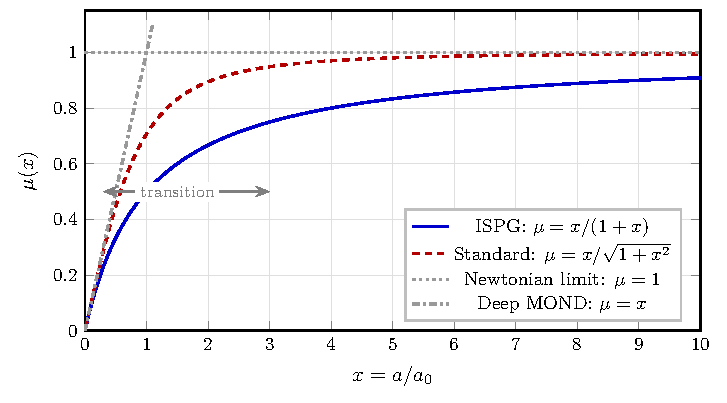
\includegraphics[width=0.75\textwidth]{PDF/fig_mond_interpolation.pdf}
\caption{MOND interpolating functions.  The solid curve
is the model result $\mu = x/(1+x)$; the dashed curve is
the ``standard'' function
$\mu = x/\sqrt{1+x^{2}}$.  Both approach unity for
$x \gg 1$ (Newtonian regime) and linearity for $x \ll 1$
(deep-MOND regime).
\label{fig:mu}}
\end{figure}

%-------------------------------------------------------------------
\subsection{Tully--Fisher relation}\label{sec:TF}
%-------------------------------------------------------------------

For a circular orbit ($a = v^{2}/r$,
$a_{N} = GM/r^{2}$) in the deep-MOND regime
$\mu(x) \approx x$, the modified dynamics
$\mu(a/\azero)\cdot a = a_{N}$ gives
$a^{2}/\azero = GM/r^{2}$.  With $a = v^{2}/r$:
\begin{equation}\label{eq:TF}
  \boxed{v^{4} = \azero\,G\,M\,,\qquad
    v_{\mathrm{flat}} = (\azero\,G\,M)^{1/4}\,.}
\end{equation}
This is the baryonic Tully--Fisher
relation~\cite{TullyFisher1977,McGaugh2016}, here
obtained in the deep-MOND limit.

\begin{figure}[t]
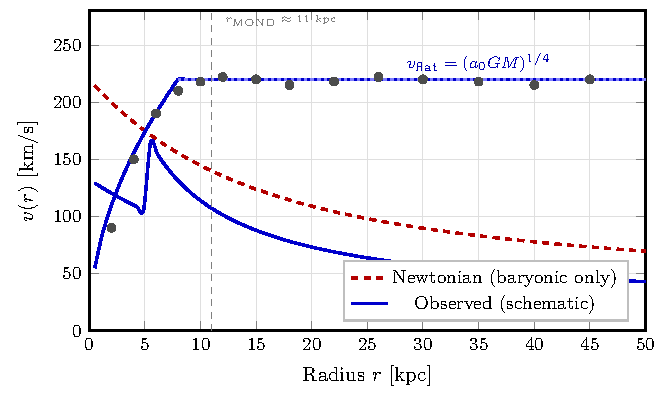
\includegraphics[width=0.75\textwidth]{PDF/fig_rotation_curve.pdf}
\caption{Schematic galaxy rotation curve.  The dashed curve
shows the Newtonian prediction from baryonic mass alone;
the solid curve represents the observed flat profile.  In the
present theory the transition occurs at
$r_{\mathrm{MOND}} \approx \sqrt{GM/\azero}$, and the
asymptotic velocity is $v_{\mathrm{flat}} = (\azero\,GM)^{1/4}$,
obtained from the deep-MOND relation with no
galaxy-by-galaxy fit parameters.
\label{fig:rotation_curve}}
\end{figure}

%-------------------------------------------------------------------
\subsection{Redshift evolution}\label{sec:a0z}
%-------------------------------------------------------------------

Since $\azero$ is set by the global pressure history, whose
observational proxy is the Hubble rate, at redshift $z$
the relevant rate is $H(z)$:
\begin{equation}\label{eq:a0z}
  \boxed{\azero(z) = \frac{c\,H(z)}{2\pi}\,.}
\end{equation}
This is the \emph{instantaneous baseline law}: it gives the coherence-set
value associated with the background Hubble rate at the observation epoch.
Galaxies therefore do react to the global pressure decrease that is
usually read observationally as cosmic expansion: the same background
shift changes their clock rate, rod scale, effective mass scale, and the
coherence-set value of $\azero$.  The full galactic prediction is slightly
more refined: the companion MOND paper~\cite{Lotishvili2026MOND} shows that
finite vortex memory replaces $H(z)$ by a lifetime-averaged
$H_{\rm eff}$, so the effective observed value is
$\azero^{\rm eff}=cH_{\rm eff}/(2\pi)$.  Equation~\eqref{eq:a0z} is
therefore the zeroth-order redshift law, recovered for newly formed
vortices and as the baseline coherence scale entering the local closure.
In $\Lambda$CDM,
$H(z) = H_{0}\sqrt{\Omega_{\mathrm{m}}(1+z)^{3}
+ \Omega_{\Lambda}}$, so the instantaneous baseline
$\azero(z)$ grows monotonically with $z$.  At $z = 1$ the
baseline ratio is $\azero(1)/\azero(0) \approx 1.78$,
predicting ${\sim}16\%$ higher flat rotation velocities at
fixed baryonic mass.  The full vortex-lag prediction is
weaker and depends on formation epoch~\cite{Lotishvili2026MOND},
but the central distinction from standard MOND remains:
$\azero$ is not constant.
This distinguishes the present theory
from standard MOND (which assumes constant $\azero$)
and is testable with high-redshift rotation curves from
JWST~\cite{JWST2023} and the baryonic Tully--Fisher
relation measured by Euclid~\cite{Euclid2024}.

\textit{Robustness of the baryonic-mass comparison.}---The
prediction ``at fixed baryonic mass'' is operationally
well-defined because the local undetectability
principle (Sec.~\ref{sec:variable_mass}) ensures that
mass-to-light ratios are independent of the conformal
factor.  Whether one works in the FLRW frame
($\varphi_0=0$, constant bare masses, expanding scale
factor) or in the ontologically preferred
matter-contraction description where coordinate
distances are fixed and effective masses and atomic
length scales rescale with the global pressure
(Sec.~\ref{sec:variable_mass}), the dimensionless
Tully--Fisher observable $v^4/(GM_{\mathrm{obs}})$
is invariant.
The prediction~(\ref{eq:a0z}) therefore requires no
separate accounting for cosmological mass evolution.

\begin{figure}[t]
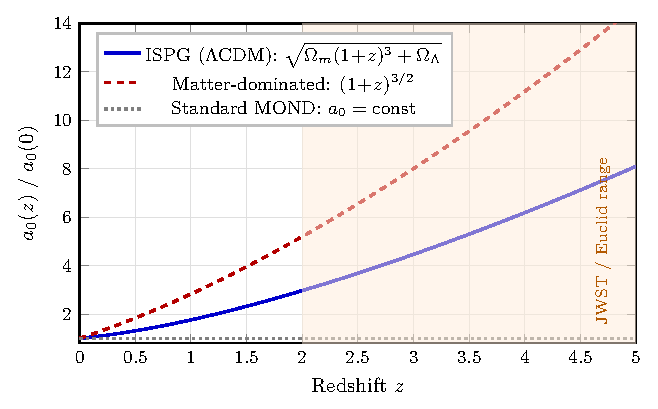
\includegraphics[width=0.75\textwidth]{PDF/fig_a0_evolution.pdf}
\caption{Redshift evolution of the critical acceleration
$\azero(z)/\azero(0)$.  The solid curve assumes
$\Lambda$CDM expansion history; the dotted line shows
matter domination.  Standard MOND (horizontal dashed)
assumes $\azero = \mathrm{const}$.  The shaded region
indicates the JWST/Euclid observational window.
\label{fig:a0z}}
\end{figure}

%-------------------------------------------------------------------
\subsection{Disk formation from rotational anisotropy}
\label{sec:disk_formation}
%-------------------------------------------------------------------

The same off-diagonal rotational anisotropy associated with
the bound-structure MOND sector also predicts the formation
of galactic disks.  The detailed rotating-medium closure is
developed in the companion MOND paper~\cite{Lotishvili2026MOND}; here we record only its geometric
consequence.
The gravitomagnetic metric component
$g_{t\phi} \propto \sin^{2}\theta$ is maximal in the
equatorial plane and vanishes on the polar axis.
The transported channel $\varphi_{h}$ inherits this
anisotropy, generating a vertical restoring acceleration
$g_{z} \propto -z/\rho$ toward the midplane with
oscillation frequency $\nu_{z}^{2} \sim 2\azero/\rho$.
The resulting disk scale height is
\begin{equation}\label{eq:disk_height}
  h \sim \sigma_{z}\sqrt{\frac{\rho}{2\azero}}\,,
\end{equation}
where $\sigma_{z}$ is the vertical velocity dispersion.
For the Milky Way at $\rho = 8\;\mathrm{kpc}$ with
$\sigma_{z} \approx 20\;\mathrm{km\,s^{-1}}$, this
gives $h \approx 0.6\;\mathrm{kpc}$, consistent with
observations.  A falsifiable prediction follows:
low-surface-brightness galaxies deep in the MOND regime
should have relatively thinner disks at fixed
$\sigma_{z}/v_{\mathrm{rot}}$ than predicted by angular
momentum conservation alone~\cite{Lotishvili2026MOND}.

%-------------------------------------------------------------------
\subsection{Status and extensions of the MOND sector}
\label{sec:mond_future}
%-------------------------------------------------------------------

The spiral-galaxy MOND closure is already fixed in the
present paper and the companion MOND paper~\cite{Lotishvili2026MOND}.  The items below summarize
that completed core result and the next extensions of the
same mechanism:

\begin{enumerate}
\item \textbf{Spiral-galaxy closure
  \emph{(completed)}.}  The interpolating function
  $\mu(x)=x/(1+x)$ and the normalization
  $a_0=cH/(2\pi)$ are now closed within the mature
  spiral-galaxy framework of the companion MOND paper~\cite{Lotishvili2026MOND}.  The
  transport-side algebraic channel is benchmarked by
  Chebyshev spectral collocation therein, while the independent source-side and
  operator-side checks are stated explicitly below at
  the $\sim10\%$ RMS level.  The local self-consistency parameter
  now obeys
  $C_{\rm eff}=A_{\rm vort}+\mathcal{O}(\delta_{\rm sp})
  +\mathcal{O}(\delta_N)$, so on the mature occupied
  branch ($Q_{\rm occ}\gg1$, $\delta_{\rm sp}\ll1$,
  $N_{\rm cell}\gg1$) one has $C_{\rm eff}\simeq1$ from
  instantaneous vortex equilibrium, and the operating transport rate
  $\Omega_{\rm tr}=a_0/c$ is fixed by the Hubble-boundary
  coherence theorem, i.e.\ by the causal
  crossing time of the Hubble coherence boundary in the
  rotating-medium field equation, while the cosmological secular integral
  supplies the background pressure-history diagnostic
  with the coupling exponent $\beta$ derived (not assumed)
  from the quantum feedback ODE.  The rotational loading law
  $Z_{\rm rot}=(1+\sqrt{X_{\rm rot}/X_0})^{-1}$ (using the local
  rotational invariant $X_{\rm rot}$ of Appendix~8, opposite sign
  to the main Horndeski $X$) is MaxEnt-selected from a
  binary free/load partition with loaded-state measure linear in
  $\sqrt{X_{\rm rot}/X_0}$, and the
  activation profile is solved self-consistently together with the
  total field rather than being evaluated on a pre-inserted MOND branch.
  The result is
  universal across galaxy parameters, converged under
  $N$-doubling, and satisfies the correct asymptotic
  limits to machine precision in the algebraic channel
  (exact given the solved $C_{\rm eff}$ profile).  The MOND transport
  sector also now admits an explicit 2D source-side
  enclosed-mass Green kernel in disk geometry with
  $\rho_{\rm core}=r_M/j_{0,1}$ fixed by regularity and
  $\kappa_G$ fixed by the outer asymptotic Gauss condition,
  and the
  transport-side spectral closure, source-side kernel,
  and operator-side AQUAL solve have now been cross-checked
  in one unified benchmark suite.  On the matched
  axisymmetric box the native field RMS errors are
  $5.7\times10^{-4}$ (transport), $1.32\times10^{-1}$
  (source-side boundary kernel), and $1.09\times10^{-1}$
  (AQUAL), while the direct source-versus-operator mismatch
  is $\simeq7.4\times10^{-2}$.  Separately, on a widened
  static axisymmetric box $(20\,r_M)\times(10\,r_M)$ where
  $\kappa_G$ is fixed on the disjoint deep-halo annulus
  $10\le\xi\le20$ and scored only on $0.3\le\xi\le10$,
  the standalone source-side and operator-side native RMS
  errors drop to $\sim1.01\times10^{-1}$ and
  $\sim9.18\times10^{-2}$, respectively, with the
  source-side transition and outer-halo subwindow RMS levels
  both staying at $\sim1.0\times10^{-1}$.  A first explicitly
  time-dependent quasi-static $2+1$D relaxation solve of
  the same source-side channel has also been carried out
  on the axisymmetric $R$--$z$ grid, and the undropped
  hyperbolic $2+1$D propagation with the $\ddot{\varphi}$
  term retained has now also been verified for the same
  derived nonlocal source-side closure.  Finally, that
  source has also been promoted from a fixed derived profile
  to a fully coupled rotating-medium law: the local
  vortex-order parameter obeys its hysteretic kinetic
  equation, the ordered tail budget is rebuilt as
  $A_{\rm vort}T^{(m)}$, and the nonlocal halo source is
  reconstructed from the enclosed coherent-budget fraction
  at every time step inside the hyperbolic $2+1$D solve.
  The fixed-source hyperbolic run remains within
  $\sim2.1\times10^{-4}$ of the selected static source-side
  branch, and the coupled run remains within
  $\sim3.8\times10^{-2}$ of
  the selected static source-side branch and within
  $\sim1.4\times10^{-1}$ of the algebraic target and
  $\sim1.2\times10^{-1}$ of the transport target, so the
  mature spiral-galaxy MOND sector is now internally consistent
  at the PDE level within its closure framework
  ($Z_{\rm rot}$, impedance-matching invariant, $\Omega_{\rm tr}=a_0/c$).
  The remaining items below are therefore
  extensions/applications of that closure rather
  than missing steps inside the spiral-galaxy derivation
  itself.
  The MOND transport
  coefficient and the background medium-pressure history
  ($w_{\rm bg} > -1$, the reservoir-side bookkeeping rather
  than the observable echo-background $w_{\rm DE}< -1$)
  are linked by the master formula
  $3\delta w_0(1+z_f)^\alpha/\alpha\approx 8$,
  yielding a DESI/Euclid consistency target.

\item \textbf{Elliptical galaxies.}  The companion MOND
  paper~\cite{Lotishvili2026MOND} now shows that
  pressure-supported systems (ellipticals, dwarf
  spheroidals) obey the same MOND scaling through a
  turbulent micro-vortex mechanism: the isotropic
  velocity dispersion $\sigma$ generates a Reynolds-stress
  analogue in the scalar field, with the transition at
  $g\sim a_0$ fixed by the cosmological coherence length.
  The predicted relation $\sigma^4 = K_\sigma\,GMa_0$
  (baryonic Faber--Jackson) is consistent with observations;
  the companion paper now also makes the normalization
  convention explicit by separating the exact global
  deep-MOND virial coefficient from the projected
  S\'ersic/aperture coefficient.  What remains open is the
  full convective-cell PDE derivation of the detailed
  projected kinematics.

\item \textbf{Galaxy clusters.}  Standard MOND
  underpredicts cluster masses by a factor
  ${\sim}2$--$3$~\cite{Angus2008}.  The IS relaxation
  mechanism (Sec.~\ref{sec:dm}) addresses the Bullet
  Cluster mass--light offset, and the companion MOND
  paper~\cite{Lotishvili2026MOND} now gives a
  quantitative benchmark for the residual cluster
  binding.  The required scalar-field retention time for
  50\% binding is $\tau_{\rm ret}^{(50\%)}\approx
  0.42\,t_{\rm dyn}$---less than half of one dynamical
  time, naturally achievable in a gravitationally bound
  system.  The corresponding effective mean free path
  $\ell_{\rm mfp}\approx 16$~kpc matches the observed
  scale of ICM cold fronts and sloshing spirals, which
  provide a concrete, parameter-free scattering mechanism.
  What remains is a dedicated 3D numerical solve of
  the scalar-field energy density on a realistic cluster
  potential, which is a computational task rather than a
  conceptual gap.

\item \textbf{Explicit regime matching.}  The physical
  separation between the linear FLRW sector and the
  nonlinear quasi-static sector is already built into the
  pressure-medium interpretation used throughout the
  theory.  A dedicated matching calculation would make
  this separation explicit in a single equation-level
  bridge across the two regimes.
\end{enumerate}

%===================================================================
\section{Physical interpretation: inertia, mass equivalence,
  effective mass, and the invariance of $c$}\label{sec:interpretation}
%===================================================================

The preceding sections derived the quantitative predictions
of the theory.  Here we draw out three physical consequences
of the bi-conformal scalar-tensor structure that bear on
foundational issues: the dynamical origin of inertia, the
identity of gravitational and inertial mass, and the local
invariance of the speed of light.

%-------------------------------------------------------------------
\subsection{Inertia as scalar-field backreaction}
\label{sec:inertia}
%-------------------------------------------------------------------

In Newtonian mechanics, inertia is an intrinsic, passive
property of matter.  In GR, it is geometrized through the
geodesic equation, but the question of \emph{why} matter
resists acceleration receives no deeper answer than the
structure of the metric itself.

In the present theory the scalar field $\varphi$ provides
a dynamical mechanism for both gravitational attraction
and inertial resistance.  Section~\ref{sec:deflection}
showed that free-fall itself is matter-wave refraction:
every oscillon turns toward regions of lower
$c_{\mathrm{coord}}$
(Eq.~\ref{eq:accel_refraction}).  Inertia is the
complementary transient effect.  A body of mass $M$ at
rest in a static background maintains the spherically
symmetric configuration $\varphi = -\rs/r$.  When the body
accelerates, this configuration must readjust.  Because
$\varphi$ propagates at finite speed $c$
(Sec.~\ref{sec:gw_speed}), the readjustment is not
instantaneous: during the transient the scalar-field
gradient develops a fore--aft asymmetry that opposes
the acceleration.

The effect is the field-theoretic analog of hydrodynamic
\emph{added mass}: a body accelerating through a fluid
experiences a retarding force because the fluid must
rearrange around it~\cite{LambHydro}.  Here the ``fluid''
is the scalar field, and the retarding force is what we
identify as inertia.

In the weak-field limit the gravitational force on a
test particle in an external potential
$\varphi_{\mathrm{ext}}$ is
\begin{equation}\label{eq:F_grav}
  \mathbf{F}_{\mathrm{grav}}
  = -m\,\nabla\varphi_{\mathrm{ext}}\,,
\end{equation}
where $m$ is the gravitational mass determined by the
particle's own contribution to the field via
Eq.~(\ref{eq:box_phi}).  When the same particle
accelerates through its own field, the transient
asymmetry $\delta\varphi$ creates a backreaction
\begin{equation}\label{eq:F_inertial}
  \mathbf{F}_{\mathrm{inertial}}
  = -m\,\nabla(\delta\varphi)\,,
\end{equation}
with the \emph{same} coupling $m$, since both
expressions derive from the same
Lagrangian~(\ref{eq:action}).  This universality of
coupling is what the next subsection formalizes as the
identity of gravitational and inertial mass.

%-------------------------------------------------------------------
\subsection{Identity of gravitational and inertial mass}
\label{sec:mass_identity}
%-------------------------------------------------------------------

The equality $m_{g} = m_{i}$ is one of the most precisely
tested facts in physics: the E\"otv\"os parameter is
constrained to $\eta < 10^{-15}$ by the MICROSCOPE
experiment~\cite{MICROSCOPE2022}.  In GR with minimally
coupled matter the equality is automatic at the
Lagrangian level: matter couples to a single metric with
a single mass parameter, and gravitational and inertial
responses inherit that same parameter.  The same is true
in ISPG; the additional structural content here is that
the common mechanism is identified explicitly---both
responses are mediated by the same scalar field
$\varphi$ through the same field equation.

\textit{Gravitational mass.}---A body placed in an
external gradient $\nabla\varphi_{\mathrm{ext}}$
experiences a force which, in the weak-field Newtonian
limit, takes the form
$F = -m\,\nabla\Phi_{N}$ with
$\Phi_{N} = \tfrac{1}{2}c^{2}\varphi$
(Sec.~\ref{sec:newton_recovery}); equivalently
$F = -\tfrac{mc^{2}}{2}\,\nabla\varphi_{\mathrm{ext}}$.
The coupling $m$ is fixed by the source term in the
field equation~(\ref{eq:box_phi}): it is the body's
contribution to the trace $T$ of the energy-momentum
tensor.  The schematic shorthand
$F = -m\,\nabla\varphi_{\mathrm{ext}}$ used informally
elsewhere should be understood with the implicit
$c^{2}/2$ factor reinstated.

\textit{Inertial mass.}---A body undergoing acceleration
$\mathbf{a}$ generates a transient field asymmetry
$\delta\varphi$.  The restoring force is
$F = -m\,\nabla(\delta\Phi_{N})
   = -\tfrac{mc^{2}}{2}\,\nabla(\delta\varphi)$,
with the same coupling $m$, because the field equation
that governs $\delta\varphi$ is the same equation that
determines the static configuration.

Since both forces derive from the same
action~(\ref{eq:action}) with minimal coupling of matter
to the bi-conformal metric, the proportionality constant
relating force to field gradient (gravitational mass) is
identically equal to the proportionality constant
relating force to acceleration (inertial mass).  The
equality $m_{g} = m_{i}$ is therefore a structural
consequence of the unified scalar-field mechanism in
ISPG; the result has the same logical status as in GR
with minimal coupling, and the additional ISPG content
is the explicit identification of the common mechanism
(retarded scalar self-field) rather than a stronger
derivation.
The retarded self-field calculation is carried out
explicitly in Appendix~17, which derives Newton's
second law $F = ma$ from the field equations.  The
quantum extension~\cite{Lotishvili2026Q} provides an
independent microscopic derivation via the Bernoulli
pressure-deficit mechanism, confirming the result at
the operator level.

\textit{From test particles to composite bodies.}---The
present argument establishes $m_{g} = m_{i}$ for test
particles in an external field.  The corresponding
statement for self-gravitating composite bodies---the
strong equivalence principle, including the absence of
a Nordtvedt effect---requires the exact shift symmetry
of the scalar sector and is treated separately in
Sec.~\ref{sec:sep} (with the universal sensitivity
$s = 1/2$ established \emph{exactly} for vacuum compact
objects and at \emph{leading order} for matter-filled
bodies in Appendix~16; the exact non-perturbative
matter-filled cancellation is an open task).

\textit{Status of the $\eta$ prediction.}---Within the
order to which the present derivation is carried,
ISPG predicts $\eta = 0$ identically: no
composition-dependent deviation arises from the unified
retarded-scalar mechanism.  The MICROSCOPE bound is
therefore satisfied trivially in this approximation,
and not used here as a discriminator.  A controlled
prediction for a possible higher-order, microscopic
composition-dependent $\eta$ would require a calculation
beyond the scope of this paper and is deferred to
future work.

This result connects directly to the MOND phenomenology
of Sec.~\ref{sec:mond}.  Using
Eq.~(\ref{eq:two_channel}) with
$a_h=(\azero/a)\,a_N$, one obtains
$\mu(x)=x/(1+x)$: for $a\gg\azero$, $a_h\ll a_N$ and
$\mu\to 1$; for $a\ll\azero$, $a_h\gg a_N$ and
$\mu\approx a/\azero$.  In this reading, MOND is the
bound-structure two-channel gravitational response of the
ISPG medium, in which the baryonic Bernoulli field is
supplemented by a rotating-space channel in galactic
structures.

%-------------------------------------------------------------------
\subsection{Position-dependent effective mass}
\label{sec:variable_mass}
%-------------------------------------------------------------------

The bi-conformal structure implies that the effective mass
of a body---its gravitational influence as measured by a
distant observer---depends on the local value of the scalar
field.  Consider a particle of rest mass $m_{0}$ at rest at
a position where the scalar field takes the value $\varphi$.
Its worldline interval is $ds = c\,e^{\varphi/2}\,dt$, and
its energy as measured at spatial infinity ($\varphi = 0$) is
\begin{equation}\label{eq:m_eff}
  E_{\infty} = m_{0}\,c^{2}\,e^{\varphi/2}\,.
\end{equation}
The effective mass, defined as
$m_{\mathrm{eff}} \equiv E_{\infty}/c^{2}$, is therefore
\begin{equation}\label{eq:meff_def}
  \boxed{m_{\mathrm{eff}}(\varphi)
    = m_{0}\,e^{\varphi/2}\,.}
\end{equation}
In a gravitational field ($\varphi < 0$),
$m_{\mathrm{eff}} < m_{0}$: a body deep in a potential
well contributes less to the total gravitational mass
of the system than the same body at infinity.

\textit{Local undetectability.}---A local observer
uses clocks that tick at rate $d\tau = e^{\varphi/2}\,dt$
and rulers of proper length $d\ell = e^{-\varphi/2}\,dr$.
The locally measured rest energy of the particle is
\begin{equation}\label{eq:m_local}
  E_{\mathrm{local}} = m_{0}\,c_{\mathrm{local}}^{2}
  = m_{0}\,c^{2}\,,
\end{equation}
since $c_{\mathrm{local}} = c$ by
Eq.~(\ref{eq:c_local_meas}).  All local masses---the
test particle, the reference kilogram, the atoms in the
scale---are multiplied by the \emph{same} conformal
factor $e^{\varphi/2}$.  The ratio of any two masses is
therefore position-independent:
\begin{equation}\label{eq:mass_ratio}
  \frac{m_{\mathrm{eff},A}}{m_{\mathrm{eff},B}}
  = \frac{m_{0,A}\,e^{\varphi/2}}
         {m_{0,B}\,e^{\varphi/2}}
  = \frac{m_{0,A}}{m_{0,B}}\,.
\end{equation}
No local experiment can detect the variation of
$m_{\mathrm{eff}}$, for the same reason that no local
experiment detects the variation of the coordinate speed
of light: the measuring apparatus participates in the
same conformal rescaling as the object being measured.

\textit{Cosmological frame duality.}---The positional
result extends to the cosmological setting.  In the FLRW
frame, $\varphi_0=0$ (Sec.~\ref{sec:flrw}) and bare masses
are epoch-independent; cosmic expansion is carried entirely
by~$a(t)$.  A conformal rescaling to coordinates in which
$a\equiv1$ maps the expansion into a time-dependent
contraction of effective masses and atomic length scales.
Since every local measuring apparatus participates in the
same rescaling, no epoch-dependent experiment can distinguish
the two descriptions; all dimensionless observables---the
baryonic Tully--Fisher relation, the CMB power spectrum---are
frame-invariant (Sec.~\ref{sec:a0z}).

In the ISPG ontology, however, the two frames are not on
equal footing.  The primary background variable is the
homogeneous pressure shift
$\varphi_{\mathrm{bg}}=\ln(P_{\mathrm{stat}}/P_{\max})$;
the observed Hubble rate serves as a practical proxy for
the global rate of static-pressure
decrease~\cite{Lotishvili2026MOND}.
The ``matter-contraction'' picture---in which coordinate
distances are fixed while effective masses, atomic length
scales, and clock rates rescale with the pressure---is,
in the ISPG interpretation, the ontologically natural
description of a physical medium whose state is defined
by its local pressure.  The FLRW frame is a
mathematically equivalent reformulation whose convenience
lies in matching the standard cosmological formalism.
The two frames are observationally equivalent at the
level of dimensionless quantities; the preference for
the matter-contraction frame as the ``primary'' one is
an interpretational choice within ISPG, not a result
derived from an observation that distinguishes the two
descriptions.

\textit{Pressure-history background factor.}---For
cosmological bookkeeping the local clock--rod--mass
response is not fixed by the observed redshift alone.
The homogeneous FLRW metric scalar is set to
$\varphi_0=0$ in cosmic-time gauge (Sec.~\ref{sec:flrw});
therefore the reuse of the local bi-conformal response
with a coarse-grained pressure diagnostic
$\varphi_{\rm bg}(z)$ is a constitutive postulate of
the pressure ontology, not a direct consequence of the
isolated-source metric derivation.  The fiducial
background multiplier used for process-time and
tail-power bookkeeping is
\begin{equation}\label{eq:pressure_history_C}
  \mathcal{C}(z)
  := e^{[\varphi_{\rm bg}(z)-\varphi_{\rm bg}(0)]/2}
  = \left[
      \frac{P_{\mathrm{stat}}(z)}
           {P_{\mathrm{stat}}(0)}
    \right]^{1/2}.
\end{equation}
With this convention the common pressure-history scaling is
\begin{equation}\label{eq:early_scaling}
\renewcommand{\arraystretch}{1.4}
\begin{array}{rcll}
  m_{\mathrm{eff}}(z)/m_{\mathrm{eff}}(0)
    &=& \mathcal{C}(z), \\
  d\ell(z)/d\ell(0)
    &=& \mathcal{C}(z)^{-1}, \\
  c_{\mathrm{coord}}(z)/c_{\mathrm{coord}}(0)
    &=& \mathcal{C}(z)^{2}, \\
  (d\tau/dt)(z)\,/\,(d\tau/dt)(0)
    &=& \mathcal{C}(z), \\
  \mathcal{P}_{\mathrm{tail}}^{(\mathrm{pert})}(z)/
  \mathcal{P}_{\mathrm{tail}}^{(\mathrm{pert})}(0)
    &=& \mathcal{C}(z)^{4}.
\end{array}
\end{equation}
The last line is the perturbative conformal-exponent
scaling.  The full tail power may be multiplied by a
non-perturbative suppression factor whose background-pressure
dependence must be modeled separately.

For the MOND-closure benchmark
$P_{\mathrm{stat}}(10)/P_{\mathrm{stat}}(0)\approx9.9$,
one obtains $\mathcal{C}(10)\approx3.1$.  Thus effective
masses and process-clock rates are enhanced by about
$3.1$, matter rod scales respond reciprocally, the
coordinate light-speed factor is about $9.9$, and the
perturbative tail-power exponent factor is of order
$10^2$.  These numbers replace the older coordinate
translation that identified the pressure-history multiplier
with the redshift factor as the fiducial pressure-history
scaling.  That redshift-factor identity can be used only as
a pedagogical FLRW-to-matter-contraction dictionary for
redshift; it is not the dynamical pressure-history closure
used in the process-time and tail-power sectors.

\emph{Gauge status.}---The coordinate factor
$c_{\mathrm{coord}}\propto\mathcal{C}^2$ is a coordinate
description.  In the FLRW frame the coordinate speed of
light is constant and the spatial coordinates expand
instead.  The two descriptions are observationally
equivalent at the level of local measurements: the speed
of light measured with local rulers and clocks
(Sec.~\ref{sec:c_invariance}) remains $c$, and
dimensionless ratios are frame-independent.

\textit{Relation to the MOND coupling
ratio.}---The companion MOND
paper~\cite{Lotishvili2026MOND} derives the
pressure ratio
$P_{\mathrm{stat}}(z)/P_{\mathrm{stat}}(0)$ from the
quantum-feedback closure.  This quantity measures the
\emph{intrinsic medium-energy evolution} driven by
the depletion of the $\nu_0$-mode reservoir
and the growth of the echo background.  It is the
quantity that enters Eq.~\eqref{eq:pressure_history_C};
it should not be supplemented by an additional exact
$(1+z)^2$ conformal factor.  For observational predictions
such as the baryonic Tully--Fisher relation and the
vortex-lag effect, the relevant input is the dynamical
coupling ratio supplied by the closure, not an independent
redshift-fixed rescaling.

\textit{Gravitational binding energy.}---For a
self-gravitating system of total bare mass $M_{0}$, the
\emph{bare-mass} Komar integral (lapse $e^{\varphi/2}$
times proper volume element $e^{-3\varphi/2}$, weighted
by the rest-mass density $\rho_0$) as measured at
infinity is
\begin{equation}\label{eq:komar}
  M_{\mathrm{Komar}}^{(0)} \equiv
  \int \rho_{0}\,e^{\varphi/2}\,
  e^{-3\varphi/2}\,d^{3}x
  = \int \rho_{0}\,e^{-\varphi}\,d^{3}x\,,
\end{equation}
where the factor $e^{-3\varphi/2}$ is the proper volume
element in the spatial metric $e^{-\varphi}\delta_{ij}$.

\paragraph{Scope of Eq.~(\ref{eq:komar}).}
Equation~(\ref{eq:komar}) is the \emph{bare-mass} (or
test-matter) Komar integral: it weights the rest-mass
density $\rho_0$ by the gravitational-redshift/proper-volume
factors alone.  It coincides with the Tolman--Komar
stationary perfect-fluid mass $M_{\mathrm{Komar}}^{\mathrm{TK}}
= \int (\rho_0 + 3p/c^2)\,e^{-\varphi}\,d^3x$ in the
dust limit $p\ll\rho_0 c^2$, and is therefore adequate
for the weak-field binding-energy discussion below and
for the kinematic sensitivity argument of
Sec.~\ref{sec:sensitivity}.  For neutron-star interiors
($p/(\rho_0 c^2)\sim 0.2$--$0.3$ near the centre), the
pressure contribution $3p/c^2$ induces a correction of
order $\sim 30\%$; incorporating it into a fully
perfect-fluid sensitivity analysis is an open task
(Appendix~16, ``open tasks'').
In the weak field ($|\varphi| \ll 1$) and at leading
order in $p/(\rho_0 c^2)$:
$M_{\mathrm{Komar}}^{(0)} \approx M_{0}(1 - \langle\varphi\rangle)$,
where $M_{0} \equiv \int\rho_{0}\,d^{3}x$ (coordinate
volume) and $\langle\varphi\rangle < 0$ is the
mass-averaged potential.  The physically meaningful
comparison is with the total proper rest mass
$M_{\mathrm{proper}} \equiv \int\rho_{0}\,
e^{-3\varphi/2}\,d^{3}x \approx
M_{0}(1 - \tfrac{3}{2}\langle\varphi\rangle)$:
\begin{equation}\label{eq:binding_deficit}
  M_{\mathrm{Komar}}^{(0)} - M_{\mathrm{proper}}
  \approx \tfrac{1}{2}\,M_{0}\,\langle\varphi\rangle < 0\,,
\end{equation}
reproducing the standard gravitational binding-energy
deficit $\Delta M = -E_{\mathrm{bind}}/c^{2}$, here
arising from the scalar-field dependence of the effective
mass rather than from a separate binding-energy calculation.

\textit{Physical interpretation.}---In the scalar-field
picture, mass is not an intrinsic, immutable property
of matter.  It is a measure of the coupling between
matter and the scalar field---the rate at which a body
sources the field equation~(\ref{eq:box_phi}).  A body
in a region of strong field ($\varphi \ll 0$) sources
the field more weakly (per unit bare mass) than the
same body at infinity.  This is because the bi-conformal
metric simultaneously slows the body's internal dynamics
(time dilation $e^{\varphi/2}$) and contracts its
spatial extent (by $e^{\varphi/2}$), reducing its
effective interaction cross-section with the scalar field.
The two effects---time dilation and spatial
contraction---are reciprocal manifestations of the same
bi-conformal factor, exactly paralleling the invariance
of $c$ derived in Sec.~\ref{sec:c_invariance}.

\textit{Scalar sensitivity of compact bodies.}---For
a self-gravitating body of compactness
$\mathcal{C} \equiv GM/(c^{2}R)$, the scalar sensitivity
is defined as
\begin{equation}\label{eq:sensitivity}
  s \equiv -\frac{1}{2}\,
  \frac{\partial\ln m_{\mathrm{eff}}}
       {\partial\varphi_{\mathrm{ext}}}
  \bigg|_{\varphi_{\mathrm{ext}}=0}\,,
\end{equation}
where $\varphi_{\mathrm{ext}}$ is the external
(background) scalar field.  In Eq.~(\ref{eq:sensitivity})
the symbol $m_{\mathrm{eff}}$ denotes the gravitational
(Komar) mass of the body that controls its response to a
rigid shift of the external field, evaluated at infinity;
this is the quantity whose shift-rescaling is the subject
of the structural argument that follows.  It is
\emph{distinct} from the test-particle Killing-energy
effective mass of Eq.~(\ref{eq:meff_def}), which rescales
universally as $e^{+\delta/2}$; the two coincide with the
bare rest mass in the limit $\varphi\to 0$.  A key
structural property of the bi-conformal framework is that
the TOV pressure-gradient equation depends only on
$d\varphi/dr$, not on $\varphi$ itself; under a rigid
shift $\varphi\to\varphi+\delta$ the density and
pressure profiles are therefore strictly unchanged
(Appendix~16, Sec.~``TOV-level shift invariance'').
The coupled scalar equation in the presence of matter
carries an explicit $e^{-\varphi}$ prefactor on its
source side and is shift-invariant only at leading order
in $|\varphi|$ (Appendix~16,
Sec.~``Coupled-system shift symmetry'').  At leading order
in $|\varphi|$ the bare-mass Komar integrand
$\rho_0\,e^{-\varphi}$ combines the universal conformal
redshift $e^{\varphi/2}$ with the proper spatial-volume
factor $e^{-3\varphi/2}$ (Appendix~16,
Eqs.~``komar\_app16'' and ``s\_kinematic''); under the
approximate rigid shift this gives the kinematic Komar
response $\partial\ln M_{\mathrm{Komar}}/\partial
\varphi_{\mathrm{ext}}=-1$ and therefore selects
\begin{equation}\label{eq:s_leading}
  s = 1/2\qquad
  \text{(leading order in $|\varphi|$, all bodies;
  Appendix~16).}
\end{equation}
The physically measurable \emph{excess} sensitivity is
then
\begin{equation}\label{eq:s_excess}
  s_{\mathrm{excess}} \equiv s - \tfrac{1}{2}
  = 0 + O(|\varphi|)\,,
\end{equation}
which is \emph{exact} for vacuum compact objects (from
$\nabla^2\varphi = 0$, main theory Sec.~7 and
Appendix~1) and holds at leading order in $|\varphi|$
for matter-filled bodies.  An exact, non-perturbative
cancellation of the residual $O(|\varphi|)$ correction
between bodies of arbitrary compactness is \emph{not}
established by the classical coupled equations and is
an open task (Appendix~16).

At the leading-order level, $s_{A} \simeq s_{B} \simeq
1/2$ for every pair, so the scalar dipole moment of
any binary is suppressed: $(s_{A}-s_{B})^{2} \simeq 0$.
The scalar dipole radiation channel is therefore not
expected to dominate over the tensor quadrupole in
binaries of moderate compactness---consistent with the
non-detection of anomalous decay in pulsar-timing and
LIGO/Virgo data (Sec.~\ref{sec:dipole}).  This is the
leading-order counterpart of local undetectability:
because the bare-mass Komar weight
$\rho_0\,e^{-\varphi}=\rho_0\,e^{\varphi/2}\,e^{-3\varphi/2}$
is built from universal factors (the conformal redshift
$e^{\varphi/2}$ and the proper-volume element
$e^{-3\varphi/2}$) common to all bodies, every body
responds identically to a background field shift at
leading order, and the differential (observable) response
is small.  The weak equivalence principle is exactly
preserved (all test particles follow geodesics of
$g_{\mu\nu}$); the strong equivalence principle is
preserved in the scalar sector at leading order, with
the exact statement contingent on closure of the open
task above.
The derivation, the coupled linearisation, the
sectoral no-hair scope, and a confrontation with
pulsar-timing bounds are developed in Appendix~16.

%-------------------------------------------------------------------
\subsection{Local invariance of the speed of light}
\label{sec:c_invariance}
%-------------------------------------------------------------------

The bi-conformal metric~(\ref{eq:metric}) implies a
position-dependent coordinate speed of light.
From $ds^{2} = 0$ along a radial null ray:
\begin{equation}\label{eq:c_coord}
  \frac{dr}{dt} = c\,e^{\varphi}\,.
\end{equation}
Near a gravitating body ($\varphi < 0$), light propagates
more slowly in coordinate terms.

A local observer, however, measures time with a clock
whose proper rate is $d\tau = e^{\varphi/2}\,dt$, and
distance with a ruler whose proper length element is
$d\ell = e^{-\varphi/2}\,dr$.  The locally measured
speed is therefore
\begin{equation}\label{eq:c_local_meas}
  c_{\mathrm{meas}}
  = \frac{d\ell}{d\tau}
  = \frac{e^{-\varphi/2}\,dr}{e^{\varphi/2}\,dt}
  = e^{-\varphi}\cdot c\,e^{\varphi}
  = c\,.
\end{equation}
The bi-conformal structure guarantees that local
measurements of the speed of light are invariant, while
the coordinate propagation speed varies with position.
The two conformal factors $e^{\varphi}$ (temporal) and
$e^{-\varphi}$ (spatial) are not independent---they are
the unique combination that produces
$\gamma = \beta = 1$ (Sec.~\ref{sec:ppn})---and their
ratio exactly cancels in any local velocity measurement.

\begin{figure}[t]
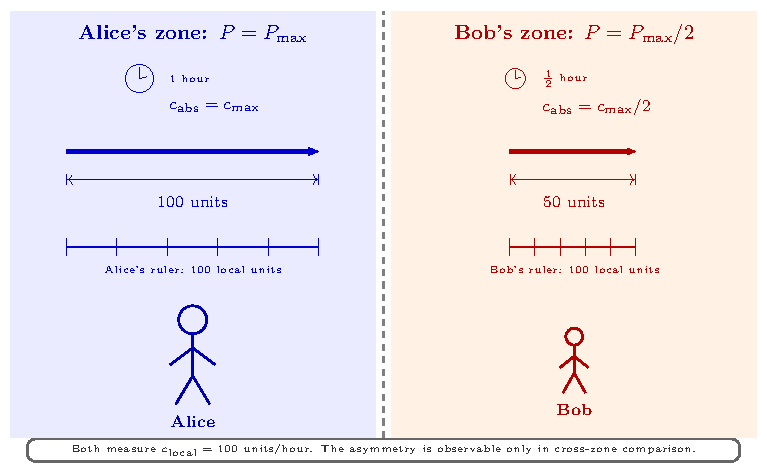
\includegraphics[width=0.75\textwidth]{PDF/fig_alice_bob.pdf}
\caption{Thought experiment illustrating local invariance of
$c$.  Alice (strong field, large $|\varphi|$ with
$\varphi=-\rs/r<0$) and Bob (weak field,
$\varphi\simeq 0$) each measure the speed of light with
local rods and clocks.  Both obtain $c$ exactly, because
the bi-conformal factors $e^{\varphi}$ and $e^{-\varphi}$
cancel in the ratio $\Delta x/\Delta t$.  A distant observer,
however, sees Alice's light travel more slowly in coordinate
terms.
\label{fig:alice_bob}}
\end{figure}

A sharper consequence emerges when one distinguishes
scalar from tensor perturbations.  A \emph{static or
adiabatically slow} change in the scalar background
($\delta\varphi$ uniform on the experiment scale,
varying on timescales much longer than the apparatus
response time) rescales the metric isotropically: clocks,
rulers, and light all respond together, rendering this
quasi-static perturbation locally undetectable.  This is
why a Michelson--Morley-type
experiment~\cite{MichelsonMorley1887} returns a null
result in a scalar-field background: the interferometer
arms adapt to the same field that governs the
propagation of light.  This is the ISPG realization
of the general fact that any metric theory with
universal minimal coupling of matter to a single metric
returns a null Michelson--Morley result; the framing
above is an explicit identification of the isotropic
scalar mode as the mode that does the compensating, not
a prediction unique to ISPG.  A \emph{dynamic}, GW-band
oscillation $\delta\varphi(t,\vec x)$ traversing the
detector at the speed of light is, by contrast, not
adiabatic with respect to the apparatus and is the
breathing mode $h_{b}$ discussed in
Sec.~\ref{sec:breathing}; this propagating scalar
perturbation does produce a measurable isotropic strain
(suppressed by source and antenna geometry as discussed
there), and the regime/gauge distinction between it and
the quasi-static null-result case is essential.

Gravitational waves, by contrast, are
transverse-traceless tensor perturbations satisfying
$\delta\varphi = 0$: they distort spatial distances
anisotropically without altering the scalar field.
Since the measuring apparatus adapts only to changes
in $\varphi$, and $\varphi$ is unchanged, the apparatus
does \emph{not} compensate.  The anisotropic strain
is therefore physically measurable---precisely the
effect detected by LIGO~\cite{LIGO2016}.

The theory thus offers a unified account: the null result
of Michelson--Morley (isotropic scalar perturbation
$\to$ compensated) and the positive detection of
gravitational waves (anisotropic tensor perturbation,
$\delta\varphi = 0$ $\to$ not compensated) both follow
from the same bi-conformal
structure~(\ref{eq:metric}).

%===================================================================
\section{Discussion}\label{sec:discussion}
%===================================================================

%-------------------------------------------------------------------
\subsection{How do local systems know about $H_{0}$?}
\label{sec:nonlocality}
%-------------------------------------------------------------------

Any framework that links a galactic quantity ($\azero$) to
a cosmological one ($H_{0}$) faces the question: through
what mechanism does the Hubble rate enter local dynamics?

In this theory no additional signal transfer is postulated.
The scalar field satisfies $\Box\varphi = 0$ on the full
spacetime, and on FLRW the term $3H\dot{\delta\varphi}$
in Eq.~(\ref{eq:damped}) sets the coherence scale
$\lambda_H \sim c/H$.  Local galactic dynamics inherit this
scale through boundary conditions of the global solution,
not through causal communication from the horizon.

%-------------------------------------------------------------------
\subsection{The dark matter question}\label{sec:dm}
%-------------------------------------------------------------------

At linear order (Sec.~\ref{sec:cmb}) the theory is GR-like,
so CMB fitting uses the same effective depth of potential
wells as $\Lambda$CDM.  The non-linear sector then sets the
scale dependence through the IS relaxation time
$\tau_{\mathrm{IS}} = c/a_{\mathrm{grav}}$.

For CMB modes at $z\sim1100$,
$\tau_{\mathrm{IS}}/T_{\mathrm{osc}} \sim 10^{3}$--$10^{10}$,
so IS wells are effectively frozen during acoustic
oscillations and act as CDM-like gravitational wells.  At
galaxy scales ($\tau_{\mathrm{IS}} \sim \tau_{\mathrm{cosm}}$)
the partial response yields MOND behavior; in cluster
mergers ($\tau_{\mathrm{IS}} > \tau_{\mathrm{collision}}$)
the same memory effect yields mass--light offsets.
Quantitative CMB validation requires coupling the IS response
to the Boltzmann hierarchy; this remains ongoing work.

\textit{Bullet Cluster mass--light offset.}---The
1E~0657--56 system (Bullet Cluster)~\cite{Clowe2006} exhibits
a spatial separation between the X-ray-emitting gas
(which decelerated at the collision center) and the
weak-lensing mass peaks (which track the galaxies on
the outskirts).  In the present theory this offset arises
naturally from the scalar-field relaxation time.  During
the collision, with relative velocity
$v_{\mathrm{coll}} \sim 3000$--$4700\;\mathrm{km\,s^{-1}}$
and subcluster mass scale $M \sim 10^{14}\,M_{\odot}$, the
gravitational acceleration at the virial radius
$r_{\mathrm{vir}} \sim 1\;\mathrm{Mpc}$ is
$a_{\mathrm{grav}} \sim GM/r_{\mathrm{vir}}^{2}
\sim 10^{-11}\;\mathrm{m\,s^{-2}}$.
The relaxation time is then
$\tau_{\mathrm{IS}} = c/a_{\mathrm{grav}}
\sim 10^{19}$--$10^{20}\;\mathrm{s}
\approx 10^{2}$--$10^{3}\;\mathrm{Gyr}$,
which far exceeds the collision crossing time
$\tau_{\mathrm{cross}} = r_{\mathrm{vir}}/v_{\mathrm{coll}}
\sim 0.2$--$0.3\;\mathrm{Gyr}$.  The scalar-field configuration
therefore cannot equilibrate during the merger:
the transported (hysteretic) component $\varphi_{h}$
remains attached to the collisionless galaxies that pass
through the collision center, while the collisional gas
decelerates and stays behind.  The weak-lensing signal
traces the total scalar-field gradient
$g = g_{N} + g_{h}$, which peaks at the galaxy positions
rather than at the gas center.  The predicted
mass--light offset
$\Delta r \sim v_{\mathrm{coll}}\,\tau_{\mathrm{cross}}$
is consistent with the observed
${\sim}720\;\mathrm{kpc}$ separation.  This
is not a fit: $\tau_{\mathrm{IS}}$ is fixed by the
same transport mechanism~\cite{Lotishvili2026MOND} that yields
$\mu(x) = x/(1+x)$.  The companion MOND paper now also
contains a first explicit frozen-hysteresis convergence
benchmark: using the observed post-collision baryonic
geometry, a minimal $2$D solve yields outer peaks at the
galaxy positions with
$\kappa_{\rm peak}/\kappa_{\rm center}\simeq2.1$ and
$250\;\mathrm{kpc}$ aperture masses
$\sim9\times10^{13}\,M_\odot$ per outer peak for an
order-unity transported hysteretic mass per side; even
outer-peak dominance already requires only
$M_\chi/M_{\rm sub}\sim0.2$--$0.4$.

\textit{Disk formation from rotational anisotropy.}---The
off-diagonal metric component $g_{t\phi} \propto \sin^{2}\theta$
vanishes on the polar axis and is maximal in the equatorial
plane.  The transported channel $\varphi_{h}$ inherits this
anisotropy, creating a $z$-directed restoring force
$g_{z} \propto -z/\rho$ toward the midplane.
This predicts a vertical oscillation frequency
$\nu_{z}^{2} \sim 2a_{0}/\rho$ and a disk scale height
$h \sim \sigma_{z}\sqrt{\rho/(2a_{0})}$, yielding
$h \approx 0.6\;\mathrm{kpc}$ for Milky-Way parameters---consistent with the observed thin disk.  The full
derivation and a falsifiable disk-thickness--rotation
correlation are given in the companion MOND paper~\cite{Lotishvili2026MOND}.

%-------------------------------------------------------------------
\subsection{Relation to other approaches}\label{sec:comparison}
%-------------------------------------------------------------------

\begin{table}[ht]
\caption{Comparison with MOND-related theories after the companion MOND analysis.
\label{tab:comparison}}
\centering
\scriptsize
\resizebox{\textwidth}{!}{%
\begin{tabular}{lcccccl}
\toprule
& \rotatebox{70}{\textbf{$\azero$ derived?}}
& \rotatebox{70}{\textbf{$\mu(x)$ derived?}}
& \rotatebox{70}{\textbf{No DM particle?}}
& \rotatebox{70}{\textbf{Cosmo.\ = GR?}}
& \rotatebox{70}{\textbf{Clusters?}}
& \textbf{Unique prediction} \\
\midrule
Standard MOND
  & no  & no  & yes & no  & no
  & EFE \\
TeVeS / AQUAL
  & no  & no  & yes & no  & no
  & $c_T\neq c$ (ruled out) \\
Verlinde
  & partly & no  & yes & unclear & partly
  & entropic DM profile \\
Superfluid DM
  & no  & partly$^{*}$ & no  & no  & yes
  & vortex lattice, phase trans. \\
Singh (2026)
  & partly & no  & yes & yes & ---
  & $\azero\propto\ell_{\rm dS}^{-1}$ \\
\textbf{ISPG}
  & \textbf{yes} & \textbf{yes} & \textbf{yes} & \textbf{yes}
  & \textbf{yes}
  & \textbf{age-dependent $\azero$} \\
\bottomrule
\end{tabular}
}
\smallskip\noindent{\footnotesize $^{*}$Superfluid DM derives
  $\mu(x)=x/\sqrt{1+x^2}$ rather than the observationally preferred
  $x/(1+x)$.}\\
\noindent{\footnotesize The ISPG entries use the companion MOND paper~\cite{Lotishvili2026MOND}: the bound-structure closure $a_h/a_N=a_0/a$, the vortex-lag correction $\azero^{\rm eff}=cH_{\rm eff}/(2\pi)$, the disk-formation result (Sec.~\ref{sec:disk_formation}), the Bullet Cluster offset (Sec.~\ref{sec:dm}), and the cluster-binding benchmark all belong to that completed nonlinear galactic sector.}
\end{table}

\begin{figure}[t]
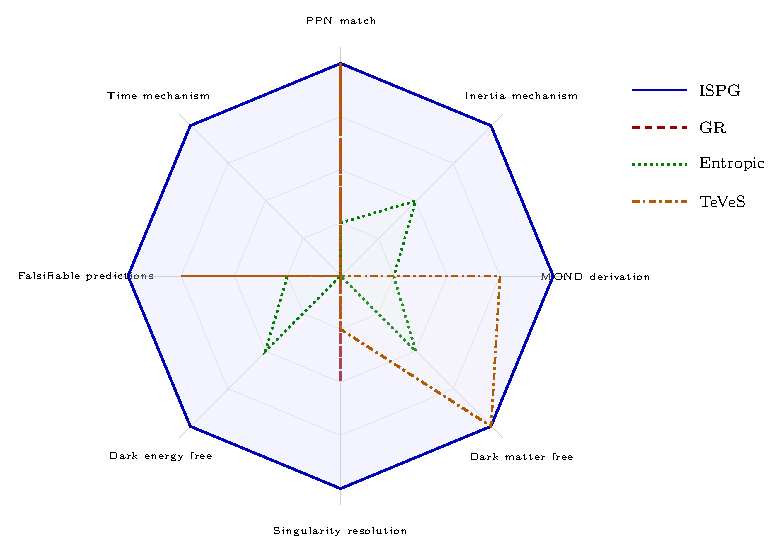
\includegraphics[width=0.75\textwidth]{PDF/fig_radar_chart.pdf}
\caption{Radar chart comparing key theoretical properties within the
legacy four-theory subset (MOND, TeVeS, $\Lambda$CDM, and ISPG):
PPN consistency, GW speed, CMB compatibility, MOND limit,
singularity resolution, and number of free parameters.
The present theory (solid) is the only framework in this subset
that spans all six criteria.
\label{fig:radar_chart}}
\end{figure}

\textit{Relation to the Fisher--Bronnikov solution
family.}---The action~(\ref{eq:action}) and exponential
metric~(\ref{eq:metric_static}) are known members of the
Fisher/JNW and Bronnikov--Ellis solution families
(\cite{Fisher1948,JNW1968,Bronnikov1973,Ellis1973,Papapetrou1954,Yilmaz1958,Boonserm2020}).
The contribution here is phenomenological extraction from this
sector: (i)~$\azero = cH_{0}/(2\pi)$ with
$\mu(x)=x/(1+x)$ from the mature rotating-galaxy
Bernoulli$+$vortex closure and the corresponding
Tully--Fisher law;
(ii)~falsifiable predictions (structurally distinct 2PN Shapiro
signature; ISCO at $\phigr^{2}\rs$; breathing-mode amplitude;
$\azero(z)$ evolution); and
(iii)~the consistency argument fixing the phantom coupling
$\kappa=-1/2$.

%-------------------------------------------------------------------
\subsection{Strong equivalence principle}\label{sec:sep}
%-------------------------------------------------------------------

The weak equivalence principle (WEP) is exactly
satisfied: all test particles follow geodesics of
$g_{\mu\nu}$ regardless of composition.  In generic
scalar-tensor theories (Brans--Dicke, DEF), the strong
equivalence principle (SEP) is violated because
self-gravitating bodies acquire compactness-dependent
scalar sensitivities $s(\mathcal{C})$, leading to
the Nordtvedt effect and scalar dipole radiation.

The bi-conformal theory possesses a sub-sectoral
\emph{shift invariance} (Appendix~16): the hydrostatic
pressure-gradient equation depends on $d\varphi/dr$,
not on $\varphi$ itself, so under $\varphi \to \varphi +
\delta$ the internal structure $\{\rho(r),\,p(r)\}$ is
strictly unchanged.  The coupled scalar equation carries
an explicit $e^{-\varphi}$ prefactor in matter and is
shift-invariant only at leading order in $|\varphi|$.
Combined with the bare-mass Komar integrand
$\rho_0\,e^{-\varphi} = \rho_0\,e^{\varphi/2}\,e^{-3\varphi/2}$
(universal conformal redshift $e^{\varphi/2}$ together
with the proper-volume factor $e^{-3\varphi/2}$;
Appendix~16, Sec.~``Kinematic motivation''), this gives
$s = 1/2$ for every body at leading order, and
\begin{equation}\label{eq:s_excess_sep}
  s_{\mathrm{excess}} = 0 \quad
  \text{(leading order; exact for vacuum compact
  objects)}.
\end{equation}
The SEP is therefore \emph{preserved in the scalar
sector at leading order}; whether the residual
$O(|\varphi|)$ correction cancels exactly body-to-body
at arbitrary compactness is an open task (Appendix~16).

Three observational consequences follow (at the
leading-order level used throughout):
\begin{enumerate}
\item \textbf{Nordtvedt effect.}  The fractional
  acceleration difference between two bodies in an
  external field is
  \begin{equation}\label{eq:nordtvedt}
    \frac{\Delta a}{a} = s_{\mathrm{excess},A}
    - s_{\mathrm{excess},B} \simeq 0\,.
  \end{equation}
  This is consistent with the Lunar Laser Ranging
  bound $|\Delta a/a| < 1.3\times10^{-13}$~\cite{Williams2004}
  and with the PSR~J0337+1715 triple-system bound
  $|\Delta a/a| < 2.6\times10^{-6}$~\cite{Archibald2018}
  (conservative 2018 value; the 2025 Voisin et al.\
  re-analysis~\cite{Voisin2025} tightens this to
  model-dependent $|\Delta|\lesssim 1.5$--$2.3\times10^{-6}$).
  Consistency with the latter at full precision requires
  closure of the open task of Appendix~16 with
  $s_{\mathrm{excess}}\to 0$ to the required accuracy.

\item \textbf{Scalar dipole radiation.}  Since
  $(s_{A} - s_{B})^{2} \simeq 0$ at leading order, the
  scalar dipole channel is strongly suppressed in every
  binary system (Sec.~\ref{sec:dipole}).  The orbital
  decay is quadrupolar-dominated, qualitatively
  consistent with PSR~J1738+0333~\cite{Freire2012}
  (illustrative pulsar bound, pending the ISPG-specific
  $\kappa_D$ normalization; see Appendix~16
  Sec.~``Compatibility-table footnote'') and with all
  LIGO--Virgo detections.  For BH--BH binaries the
  statement is rigorous (vacuum no-hair, the exterior
  harmonic monopole profile combined with the
  rigid-shift response of the bare-mass Komar integral).

\item \textbf{Preferred-frame effects.}  In principle,
  the scalar field selects a cosmological rest frame
  through $\varphi_{0}(t)$.  However, on the FLRW
  background $\varphi_{0} = 0$
  (Sec.~\ref{sec:flrw}), so preferred-frame PPN
  parameters ($\alpha_{1}$, $\alpha_{2}$) are expected
  to vanish at the cosmological-background level; a full
  derivation of $\alpha_{1}=\alpha_{2}=\alpha_{3}=0$
  from the matter-coupled equations would tighten this
  expectation and remains an open task (cf.\ the C.6
  caveat in Appendix~8).
\end{enumerate}

The leading-order preservation of SEP in the scalar
sector is not a tuning but a structural consequence of
the bi-conformal metric: the gravitational coupling
$G_{4}$ is constant (no Brans--Dicke running), and the
TOV pressure-gradient equation depends on
$\nabla\varphi$, not on $\varphi$.  This distinguishes
the theory from Brans--Dicke and DEF, in which
$s_{\mathrm{excess}} = O(1)$ compactness-dependent
effects drive incompatibility with pulsar-timing data.  The full derivation, the correction of a
naive perturbation analysis, and the observational
confrontation are given in Appendix~16.

%-------------------------------------------------------------------
\subsection{Extensions and open questions}\label{sec:speculative}
%-------------------------------------------------------------------

The matter-origin point below has been derived in
the quantum extension~\cite{Lotishvili2026Q}; the
dark-energy point is a conditional perturbative-branch
scale estimate, and the third point remains conjectural.

\textit{Dark energy scale (conditional).}---The quantum
extension~\cite{Lotishvili2026Q} shows that irreversible
spreading of resonant tails gives a positive outgoing
energy flux, while the resulting pressure drop weakens
sources through a negative-feedback loop.  On the
perturbative tail-power branch the equilibrium
echo-background energy density is estimated at
$\rho_{\Lambda} \sim H_{0}^{2}\Mpl^{2}$.  This addresses
the observed dark-energy scale at the branch-estimate level,
but the full zero-point decoupling and non-perturbative
normalization required for a complete cosmological-constant
solution remain open.  The predicted equation of state is
$w(z) = -1 - \delta w_{0}\,(1+z)^{3}/E(z)$ with
$\delta w_{0} \sim 10^{-2}$--$10^{-1}$ and $w < -1$
at all epochs (source-driven phantom, no ghost instability),
with the magnitude conditional on the tail-power normalization.
DESI DR2 gives a mixed CPL comparison---the sign of $w_a$
is aligned, while the sign of $w_0+1$ is opposite---so this
is a falsifiable DESI/Euclid target rather than a confirmation.

\textit{Matter origin (derived).}---Elementary
particles are identified as localized resonant
excitations (oscillons) of the scalar-metric
medium~\cite{Lotishvili2026Q}.  The mass spectrum
arises from the eigenvalues of a three-dimensional
nonlinear resonator, and the mass ratios are
determined by the cavity geometry independently of~$G$.
Planck-mass oscillons nucleate from the quiescent
medium via $O(4)$-symmetric instantons, providing
a singularity-free onset without inflation.

\textit{Black-hole information (conjectural).}---In
the bi-conformal metric the coordinate speed of light is
$c_{\mathrm{coord}} = c\,e^{\varphi}$ with
$\varphi = -\rs/r$, so $c_{\mathrm{coord}}\to 0$
as $r\to 0$ but never vanishes at finite~$r$
(the locally measured speed remains $c$;
Sec.~\ref{sec:c_invariance}).
Photons approaching the compact object are not
captured by a finite-radius horizon; they are progressively
decelerated.  Any information encoded in these
photons---spectral lines, polarization, timing---is
redshifted into an ever-slower exterior description.
In the static exterior model it is not causally hidden
behind a finite-radius horizon; actual retrieval remains
dependent on the open boundary condition or extension
at $r=0$.

The standard information paradox~\cite{Hawking1976}
arises from the combination of an event horizon (which
causally disconnects interior and exterior) and thermal
Hawking radiation (which carries no interior
correlations).  In the present exterior neither ingredient
is present in the same form: the finite-radius horizon
is absent (Sec.~\ref{sec:horizonless}), and the exponential
suppression $e^{-\rs/r}$ makes the deep interior effectively
inert without introducing such a horizon.  The usual
finite-radius event-horizon route to the paradox is therefore
absent in this exterior model, but a full information-recovery
statement remains conjectural and boundary-condition dependent.

%-------------------------------------------------------------------
\subsection{Scope and companion papers}\label{sec:limitations}
%-------------------------------------------------------------------

Core results are presented here; extended derivations are
deferred as follows:

\begin{enumerate}
\item Full MOND derivation and symbolic/numerical
  verification are collected in the companion MOND paper~\cite{Lotishvili2026MOND}; the main body
  keeps $\azero$, $\mu$, and Tully--Fisher at result level.
\item Quantitative CMB-era rotational transport and Boltzmann
  coupling are deferred (Sec.~\ref{sec:dm}).
\item Cluster dynamics: the Bullet Cluster mass--light offset
  is estimated in Sec.~\ref{sec:dm}; detailed $N$-body
  simulations with scalar-field relaxation are deferred
  to~\cite{Lotishvili2026}.
\item ADM constraint analysis and DOF counting (structural
  argument; full bracket-closure proof deferred) are in
  Appendix~11; quantum stability arguments (kinematic
  ghost freedom, structurally Abelian constraint algebra,
  and Hamiltonian boundedness within the pure-gravity
  constrained sector; matter-coupled extension via the EFT
  completion) are presented in~\cite{Lotishvili2026Q}.
\item The 2PN Shapiro discriminator is closed analytically as
  the finite ISPG--GR difference
  $\Delta B=\pi/4$ (Sec.~\ref{sec:shapiro}; Appendix~6).
  Full ray-tracing and absolute finite-endpoint coefficients
  for a chosen observational timing model remain implementation
  tasks, not open pieces of the differential benchmark.
\item Black-hole shadow prediction:
  the static spherical benchmark gives
  $b_c=e\,\rs$, a $4.6\%$ enhancement over the
  Schwarzschild critical impact parameter; image-level
  confrontation requires spin, accretion, and ray-tracing
  modelling and is future work~\cite{Lotishvili2026}.
\item Scalar sensitivity of compact bodies: the
  bi-conformal TOV equations, the kinematic argument
  selecting $s = 1/2$ at leading order in $|\varphi|$
  for all bodies, the sectoral analysis of shift
  invariance (exact for the TOV pressure-gradient
  equation; leading-order for the coupled system in
  matter; exact for vacuum compact objects), and the
  confrontation with pulsar-timing bounds are developed
  in Appendix~16.  An exact, non-perturbative cancellation
  of $s_{\mathrm{excess}}$ at arbitrary compactness is
  an open task.  The companion quantum paper conjectures
  that the classical leading-order invariance is
  promoted to an exact Ward identity of the quantised
  system~\cite{Lotishvili2026Q}.
\item The covariant hysteresis sector (memory field
  $\chi$ coupled to quasi-static $\varphi$ gradients) is formulated
  as an effective collective-field template in Appendix~13:
  field equation, ghost freedom, gradient stability,
  standalone sourced-KG well-posedness, and quasi-static
  overdamped reduction to the phenomenological relaxation law
  with effective timescale $\tau^{-1} = \lambda c^{2}/(3H)$.
  The microscopic tracking stiffness
  $\lambda_{\rm micro}$ is tied to the oscillon quasi-normal
  mode structure in~\cite{Lotishvili2026Q}, while the full
  backreacting two-field principal-symbol analysis and the
  macroscopic collective relaxation scale remain open.
\item Appendix~18 collects the pressure-history process
  time implied by the clock-rate postulate, making
  explicit the distinction between the standard FLRW
  cosmic-time description and the pressure-weighted
  pressure-weighted process time relevant for cumulative
  matter-sector histories.
\item \textbf{Quantum extension~\cite{Lotishvili2026Q}:}
  canonical quantization of the scalar-metric system,
  the Bernoulli pressure-deficit mechanism for gravity,
  reduced-gap/coercive closure of the localized source sector,
  microscopic derivation of Newton's second law and the
  microscopic motivation of the hysteresis action template
  $S_{\chi}$, vacuum energy
  self-regulation as a perturbative-branch estimate of the
  dark-energy scale, with the full cosmological-constant
  problem still open, dark-energy equation of state
  $w(z) < -1$ (source-driven phantom) as a falsifiable
  conditional branch,
  gravitational decoherence
  ($\Gamma = 2m|\Delta\Phi_N|/h$), charged-lepton
  mass spectrum and Koide formula, gravitational
  birefringence, anisotropic tunneling, and
  topological classification of spin and antimatter.
\end{enumerate}

%===================================================================
\section{Conclusion}\label{sec:conclusion}
%===================================================================

The theory is defined by the action~(\ref{eq:action}) and
bi-conformal ansatz~(\ref{eq:metric}), with no tunable
gravitational parameters beyond $G$.  Main results:

\begin{enumerate}
\item \textbf{Solar-system limit:} $\gamma=\beta=1$;
  1PN light deflection, perihelion, Shapiro delay, and
  Lense--Thirring agree with GR (Sec.~\ref{sec:solar}).

\item \textbf{2PN Shapiro (closed differential benchmark):} the bi-conformal
  exponential refractive index $n=e^{-\varphi}$ produces a
  2PN delay signature distinct from GR's rational-polynomial
  form.  The straight-line refractive sub-piece yields the exact
  coefficient $2\pi$, while the bent-ray and path-length pieces
  are common to the shared 1PN trajectory and cancel in the
  differential comparison.  The closed result is
  \[
  \Delta t_{2{\rm PN}}^{\rm ISPG}
  -\Delta t_{2{\rm PN}}^{\rm GR}
  =
  \frac{\pi}{4}\,\frac{G^2M^2}{c^5 b}
  \]
  for asymptotic endpoints, with the finite-distance arctangent
  form given in Sec.~\ref{sec:shapiro}.

\item \textbf{GW sector:} $c_g=c$ exactly;
  modes $(h_+,h_\times,h_b)$ with estimated
  $A_b/A_t\sim\rs/r$ (linear-scaling working estimate,
  motivated by $s=1/2$ universality; both the linear
  scaling and the scalar-quadrupole PN prefactor remain
  conditional on the open PN derivation in
  Appendix~10); test-particle ISCO orbital-frequency
  proxy $\approx 6.9\%$ lower than GR
  (Sec.~\ref{sec:merger}; comparable-mass waveform
  modelling and population-level confrontation flagged
  as future work).

\item \textbf{Stability (classical and quantum):} strong
  hyperbolicity, causal characteristics, no gradient
  instability; constrained background suppresses ghost
  decay channel (Sec.~\ref{sec:phantom}).  The quantum
  extension~\cite{Lotishvili2026Q} argues for all-loop
  stability within the pure-gravity constrained sector:
  structurally Abelian constraint algebra (full
  bracket-closure proof deferred), Hamiltonian
  boundedness on the constrained background, and loop
  suppression $(E/\Mpl)^{2} \sim 10^{-76}$;
  matter-coupled stability is controlled by the EFT
  completion.

\item \textbf{Bernoulli mechanism:}
  the quantum extension~\cite{Lotishvili2026Q} derives
  a static pressure
  $P_{\mathrm{static}} =
  -e^{\varphi}\varphi^{4}/(32\pi G\,\rs^{2})$
  from the Bernoulli identity of the scalar-metric
  medium on the exterior Coulomb branch.  The same scalar
  profile defines the metric that governs geodesic motion
  and carries the pressure deficit, providing a
  mechanism-level answer to why the metric is
  gravitational without introducing a separate
  pressure-gradient force on matter.  In the reduced source space,
  the non-neutral remainder is separated from zero by a
  positive spectral gap and controlled by a coercive
  energy estimate, so the far-zone field follows the
  same collective coordinate as the localized source.

\item \textbf{Compact objects:} $K\to0$ as $r\to0$,
  infinite proper radial depth, horizonless geometry,
  curvature-regular boundary at infinite redshift
  (Appendix~12), and $r_{\mathrm{ISCO}}=\phigr^2\rs$
  (Sec.~\ref{sec:singularity}).

\item \textbf{Cosmology:}
  $\alpha_K=\alpha_B=\alpha_M=\alpha_T=0$ on FLRW, hence
  linear CMB equivalence with $\Lambda$CDM
  (Sec.~\ref{sec:cmb}).

\item \textbf{Dark energy:}
  the accumulated echo background gives, on the perturbative
  tail-power branch, a self-regulated estimate
  $\rho_{\Lambda}\sim H_0^{2}\Mpl^{2}$ via irreversible
  resonant-tail spreading; the zero-point decoupling and
  non-perturbative normalization needed for a complete
  cosmological-constant solution remain open.  Equation of
  state $w(z)<-1$ at all
  epochs (source-driven phantom, no ghost instability)~\cite{Lotishvili2026Q},
  with DESI DR2 providing a mixed CPL comparison rather than
  a present confirmation
  (Sec.~\ref{sec:speculative}).

\item \textbf{Process time:}
  the clock-rate postulate implies a pressure-weighted
  cumulative duration for matter-sector process histories,
  $d\tau_{\mathrm{proc}}=
  [P_{\mathrm{stat}}(z)/P_{\mathrm{stat}}(0)]^{1/2}dt$,
  so structure formation and analogous secular processes
  can have substantially more process duration than the
  naive coordinate age measured by today's clocks
  (Appendix~18).

\item \textbf{MOND regime:}
  for mature rotating galaxies,
  $\azero=cH_0/(2\pi)$; the two-channel Bernoulli$+$vortex
  closure gives $\mu(x)=x/(1+x)$ and $v^4=\azero GM$
  (Sec.~\ref{sec:mond}).

\item \textbf{Mass equivalence and inertia:}
  $m_g=m_i$ follows from common scalar coupling; MOND is
  interpreted as modified inertia rather than modified gravity
  (Sec.~\ref{sec:interpretation}).

\item \textbf{Position-dependent effective mass:}
  $m_{\mathrm{eff}}=m_0\,e^{\varphi/2}$; locally
  undetectable because all masses scale by the same
  conformal factor; reproduces gravitational binding
  energy as a scalar-field effect
  (Sec.~\ref{sec:variable_mass}).

\item \textbf{Local light-speed invariance:}
  $c_{\mathrm{meas}}=c$ locally despite
  position-dependent coordinate speed
  (Sec.~\ref{sec:c_invariance}).

\item \textbf{Evolution test:}
  $\azero(z)=cH(z)/(2\pi)$
  (Sec.~\ref{sec:a0z}); the vortex-lag correction
  $H\to H_{\rm eff}$ predicts galaxy-age-dependent
  $\azero$~\cite{Lotishvili2026MOND}.

\item \textbf{Disk formation:}
  rotational anisotropy of the off-diagonal sector
  ($g_{t\phi}\propto\sin^2\theta$)
  generates vertical confinement toward the equatorial plane,
  predicting disk scale height
  $h\sim\sigma_z\sqrt{\rho/(2\azero)}$
  (Sec.~\ref{sec:disk_formation}; see also~\cite{Lotishvili2026MOND}).

\item \textbf{Cluster mergers:}
  scalar-field relaxation time
  $\tau_{\mathrm{IS}}=c/a_{\mathrm{grav}}\gg\tau_{\mathrm{cross}}$
  produces mass--light offsets in systems such as the
  Bullet Cluster without particle dark matter
  (Sec.~\ref{sec:dm}).

\item \textbf{Suppression of scalar dipole radiation:}
  the bare-mass Komar integrand $\rho_0\,e^{-\varphi}
  = \rho_0\,e^{\varphi/2}\,e^{-3\varphi/2}$ (combining
  the universal conformal redshift $e^{\varphi/2}$ with
  the proper-volume factor $e^{-3\varphi/2}$) selects
  $s=1/2$ at leading order in $|\varphi|$ for every
  body, so $(s_A - s_B)^2 \simeq 0$ and the scalar
  dipole channel is strongly suppressed in every
  binary---qualitatively consistent at leading order with
  pulsar-timing and LIGO--Virgo observations
  (Sec.~\ref{sec:dipole};
  Appendix~16).  For vacuum compact objects the
  cancellation is exact (the exterior harmonic monopole
  profile combined with rigid-shift response of the
  bare-mass Komar integral; Appendix~16,
  Sec.~``No-hair property: scope'', item~1);
  for matter-filled bodies, an exact non-perturbative
  cancellation is an open task.  The companion quantum
  paper conjectures a Ward-identity promotion of the
  leading-order invariance~\cite{Lotishvili2026Q}.

\item \textbf{SEP preservation in the scalar sector
  (leading order):}
  WEP is exact; the sub-sectoral shift invariance of
  the TOV pressure-gradient equation, together with the
  bare-mass Komar integrand $\rho_0\,e^{-\varphi}
  =\rho_0\,e^{\varphi/2}\,e^{-3\varphi/2}$ (combining
  the universal conformal redshift with the proper
  spatial-volume factor; Appendix~16,
  Sec.~``Kinematic motivation''), gives
  $s_{\mathrm{excess}} \simeq 0$ at leading order in
  $|\varphi|$, qualitatively consistent with all current
  pulsar-timing bounds at leading order (pending the
  Appendix~16 ISPG-specific $\kappa_D$ normalization and
  the matter-filled-body $s_{\mathrm{excess}}$ open
  task).  The exact, non-perturbative
  version of this statement at arbitrary compactness is
  an open task; the Ward-identity conjecture of the
  companion quantum paper~\cite{Lotishvili2026Q}, if
  proven, would secure it.  The mechanism distinguishes
  the theory from Brans--Dicke and DEF, where
  $s_{\mathrm{excess}} = O(1)$ (Sec.~\ref{sec:sep};
  Appendix~16).

\item \textbf{Gravitational decoherence:}
  $\Gamma_{\mathrm{dec}} = 2m|\Delta\Phi_N|/h$, a
  parameter-free prediction testable by
  matter-wave interferometry with
  $\Delta\Phi_N \sim 10^{-9}$~\cite{Lotishvili2026Q}.

\item \textbf{Scalar birefringence:}
  the bi-conformal metric predicts a polarization-dependent
  speed difference $\Delta c/c \sim (\rs/r)^2 \sim
  10^{-12}$ for propagation through a Coulomb
  profile~\cite{Lotishvili2026Q}.

\item \textbf{Koide mass relation:}
  the rank-1 bi-conformal coupling predicts the
  charged-lepton mass ratio $Q = 2/3$ (the Koide
  formula) if the self-consistent oscillon perturbation
  strength reaches $x \approx 66.9$---a condition whose
  numerical verification is the principal open
  computational test~\cite{Lotishvili2026Q}.

\item \textbf{Anisotropic tunneling:}
  tunneling rates acquire a directional dependence
  via the bi-conformal metric, with the anisotropy
  proportional to $\varphi$ at leading
  order~\cite{Lotishvili2026Q}.
\end{enumerate}

Primary falsification channels are:
(i)~2PN Shapiro delay in pulsar--BH binaries,
(ii)~LISA breathing-polarization search,
(iii)~merger-frequency offset,
(iv)~redshift evolution of the Tully--Fisher normalization,
(v)~disk-thickness--rotation correlation in
  low-surface-brightness galaxies,
(vi)~mass--light offset scaling in merging clusters,
(vii)~dark-energy equation of state $w(z)<-1$ with
  $\delta w_0\sim 10^{-2}$--$10^{-1}$
  as a conditional DESI/Euclid falsification target,
(viii)~gravitational decoherence rate in
  matter-wave interferometry, and
(ix)~scalar birefringence $\Delta c/c\sim 10^{-12}$.

\let\savedaddcontentsline\addcontentsline
\def\addcontentsline#1#2#3{}
\begin{acknowledgments}
Symbolic computations were performed with
SageManifolds~\cite{SageManifolds}.
\end{acknowledgments}
\let\addcontentsline\savedaddcontentsline

%===================================================================
% REFERENCES
%===================================================================
\ifdefined\ISPGMasterBuildFlag\else
% Consolidated bibliography for standalone and master builds
\begin{thebibliography}{99}

\bibitem{Einstein1915}
A.~Einstein,
``Die Feldgleichungen der Gravitation,''
Sitzungsber.\ Preuss.\ Akad.\ Wiss.\ Berlin, 844 (1915).

\bibitem{Will2014}
C.~M.~Will,
``The Confrontation between General Relativity and Experiment,''
Living Rev.\ Relativ.\ \textbf{17}, 4 (2014).

\bibitem{Will2018}
C.~M.~Will,
\textit{Theory and Experiment in Gravitational Physics},
2nd ed.\ (Cambridge University Press, 2018).

\bibitem{LIGO2016}
B.~P.~Abbott \textit{et al.}\ (LIGO/Virgo),
``Observation of Gravitational Waves from a Binary Black Hole Merger,''
Phys.\ Rev.\ Lett.\ \textbf{116}, 061102 (2016).

\bibitem{LIGO_GW170817}
B.~P.~Abbott \textit{et al.}\ (LIGO/Virgo/Fermi/INTEGRAL),
``Gravitational Waves and Gamma-Rays from a Binary Neutron Star Merger: GW170817 and GRB~170817A,''
Astrophys.\ J.\ Lett.\ \textbf{848}, L13 (2017).

\bibitem{TullyFisher1977}
R.~B.~Tully and J.~R.~Fisher,
``A New Method of Determining Distances to Galaxies,''
Astron.\ Astrophys.\ \textbf{54}, 661 (1977).

\bibitem{McGaugh2016}
S.~S.~McGaugh, F.~Lelli, and J.~M.~Schombert,
``Radial Acceleration Relation in Rotationally Supported Galaxies,''
Phys.\ Rev.\ Lett.\ \textbf{117}, 201101 (2016).

\bibitem{Milgrom1983a}
M.~Milgrom,
``A Modification of the Newtonian Dynamics as a Possible Alternative to the Hidden Mass Hypothesis,''
Astrophys.\ J.\ \textbf{270}, 365 (1983).

\bibitem{Milgrom1999}
M.~Milgrom,
``The Modified Dynamics as a Vacuum Effect,''
Phys.\ Lett.\ A \textbf{253}, 273 (1999).

\bibitem{Famaey2012}
B.~Famaey and S.~S.~McGaugh,
``Modified Newtonian Dynamics (MOND): Observational Phenomenology and Relativistic Extensions,''
Living Rev.\ Relativ.\ \textbf{15}, 10 (2012).

\bibitem{Angus2008}
G.~W.~Angus, B.~Famaey, and H.~S.~Zhao,
``Can MOND take a bullet? Analytical comparisons of three versions of MOND beyond spherical symmetry,''
Mon.\ Not.\ R.\ Astron.\ Soc.\ \textbf{371}, 138 (2006).

\bibitem{Bekenstein2004}
J.~D.~Bekenstein,
``Relativistic Gravitation Theory for the Modified Newtonian Dynamics Paradigm,''
Phys.\ Rev.\ D \textbf{70}, 083509 (2004).

\bibitem{Sotiriou2010}
T.~P.~Sotiriou and V.~Faraoni,
``$f(R)$ Theories of Gravity,''
Rev.\ Mod.\ Phys.\ \textbf{82}, 451 (2010).

\bibitem{BrunetonEsposito2007}
J.-P.~Bruneton and G.~Esposito-Far\`ese,
``Field-Theoretical Formulations of MOND-like Gravity,''
Phys.\ Rev.\ D \textbf{76}, 124012 (2007).

\bibitem{Penrose1965}
R.~Penrose,
``Gravitational Collapse and Space-Time Singularities,''
Phys.\ Rev.\ Lett.\ \textbf{14}, 57 (1965).

\bibitem{Hawking1970}
S.~W.~Hawking and R.~Penrose,
``The Singularities of Gravitational Collapse and Cosmology,''
Proc.\ R.\ Soc.\ Lond.\ A \textbf{314}, 529 (1970).

\bibitem{DeWitt1967}
B.~S.~DeWitt,
``Quantum Theory of Gravity. I. The Canonical Theory,''
Phys.\ Rev.\ \textbf{160}, 1113 (1967).

\bibitem{tHooft1974}
G.~'t~Hooft and M.~Veltman,
``One-Loop Divergences in the Theory of Gravitation,''
Ann.\ Inst.\ Henri Poincar\'e A \textbf{20}, 69 (1974).

\bibitem{BransDicke1961}
C.~Brans and R.~H.~Dicke,
``Mach's Principle and a Relativistic Theory of Gravitation,''
Phys.\ Rev.\ \textbf{124}, 925 (1961).

\bibitem{Horndeski1974}
G.~W.~Horndeski,
``Second-Order Scalar-Tensor Field Equations in a Four-Dimensional Space,''
Int.\ J.\ Theor.\ Phys.\ \textbf{10}, 363 (1974).

\bibitem{BelliniSawicki2014}
E.~Bellini and I.~Sawicki,
``Maximal Freedom at Minimum Cost: Linear Large-Scale Structure in General Modifications of Gravity,''
J.\ Cosmol.\ Astropart.\ Phys.\ \textbf{2014}(07), 050.

\bibitem{Bertotti2003}
B.~Bertotti, L.~Iess, and P.~Tortora,
``A Test of General Relativity Using Radio Links with the Cassini Spacecraft,''
Nature \textbf{425}, 374 (2003).

\bibitem{Williams2004}
J.~G.~Williams, S.~G.~Turyshev, and D.~H.~Boggs,
``Progress in Lunar Laser Ranging Tests of Relativistic Gravity,''
Phys.\ Rev.\ Lett.\ \textbf{93}, 261101 (2004).

\bibitem{Everitt2011}
C.~W.~F.~Everitt \textit{et al.},
``Gravity Probe B: Final Results of a Space Experiment to Test General Relativity,''
Phys.\ Rev.\ Lett.\ \textbf{106}, 221101 (2011).

\bibitem{Shapiro1964}
I.~I.~Shapiro,
``Fourth Test of General Relativity,''
Phys.\ Rev.\ Lett.\ \textbf{13}, 789 (1964).

\bibitem{Blanchet1993}
L.~Blanchet and G.~Sch\"afer,
``Gravitational Wave Tails and Binary Star Systems,''
Classical Quantum Gravity \textbf{10}, 2699 (1993).

\bibitem{BodennerWill2003}
J.~Bodenner and C.~M.~Will,
``Deflection of light to second order: A tool for illustrating principles of general relativity,''
Am.\ J.\ Phys.\ \textbf{71}, 770--773 (2003).

\bibitem{EpsteinShapiro1980}
R.~Epstein and I.~I.~Shapiro,
``Post-post-Newtonian deflection of light by the Sun,''
Phys.\ Rev.\ D \textbf{22}, 2947--2949 (1980).

\bibitem{KeetonPetters2005}
C.~R.~Keeton and A.~O.~Petters,
``Formalism for testing theories of gravity using lensing by compact objects,''
Phys.\ Rev.\ D \textbf{72}, 104006 (2005).

\bibitem{SKA2015}
M.~Kramer \textit{et al.},
``Strong-Field Tests of Gravity Using Pulsars and Black Holes,''
in \textit{Advancing Astrophysics with the Square Kilometre Array} (2015).

\bibitem{Carroll2003}
S.~M.~Carroll, M.~Hoffman, and M.~Trodden,
``Can the Dark Energy Equation-of-State Parameter $w$ Be Less Than $-1$?''
Phys.\ Rev.\ D \textbf{68}, 023509 (2003).

\bibitem{Cline2004}
J.~M.~Cline, S.~Jeon, and G.~D.~Moore,
``The Phantom Menaced: Constraints on Low-Energy Effective Ghosts,''
Phys.\ Rev.\ D \textbf{70}, 043543 (2004).

\bibitem{Sbisa2015}
F.~Sbis\`a,
``Classical and Quantum Ghosts,''
Eur.\ J.\ Phys.\ \textbf{36}, 015009 (2015).

\bibitem{Papallo2018}
G.~Papallo and H.~S.~Reall,
``On the Local Well-Posedness of Lovelock and Horndeski Theories,''
Phys.\ Rev.\ D \textbf{96}, 044019 (2017).

\bibitem{Kovacs2020}
A.~D.~Kov\'acs and H.~S.~Reall,
``Well-Posed Formulation of Scalar-Tensor Effective Field Theory,''
Phys.\ Rev.\ Lett.\ \textbf{124}, 221101 (2020).

\bibitem{Afshordi2007}
N.~Afshordi, D.~J.~H.~Chung, and G.~Geshnizjani,
``Cuscuton: A Causal Field Theory with an Infinite Speed of Sound,''
Phys.\ Rev.\ D \textbf{75}, 083513 (2007).

\bibitem{Chamseddine2013}
A.~H.~Chamseddine and V.~Mukhanov,
``Mimetic Dark Matter,''
J.\ High Energy Phys.\ \textbf{2013}(11), 135.

\bibitem{ArkaniHamed2004}
N.~Arkani-Hamed, H.-C.~Cheng, M.~A.~Luty, and S.~Mukohyama,
``Ghost Condensation and a Consistent Infrared Modification of Gravity,''
J.\ High Energy Phys.\ \textbf{2004}(05), 074.

\bibitem{SageManifolds}
E.~Gourgoulhon, M.~Bejger, and others,
``SageManifolds: Differential Geometry and Tensor Calculus with SageMath,''
\url{https://sagemanifolds.obspm.fr/} (2023).

\bibitem{EHT2022}
Event Horizon Telescope Collaboration,
``First Sagittarius~A* Event Horizon Telescope Results. I.,''
Astrophys.\ J.\ Lett.\ \textbf{930}, L12 (2022).

\bibitem{EHT2019M87}
Event Horizon Telescope Collaboration,
``First M87 Event Horizon Telescope Results. I. The Shadow of the Supermassive Black Hole,''
Astrophys.\ J.\ Lett.\ \textbf{875}, L1 (2019),
DOI: 10.3847/2041-8213/ab0ec7.

\bibitem{EHT2024M87}
Event Horizon Telescope Collaboration,
``The persistent shadow of the supermassive black hole of M87. I. Observations, calibration, imaging, and analysis,''
Astron.\ Astrophys.\ \textbf{681}, A79 (2024),
DOI: 10.1051/0004-6361/202347932.

\bibitem{Cardoso2019}
V.~Cardoso and P.~Pani,
``Testing the Nature of Dark Compact Objects: A Status Report,''
Living Rev.\ Relativ.\ \textbf{22}, 4 (2019).

\bibitem{Miani2023}
A.~Miani \emph{et al.},
``Constraints on the amplitude of gravitational wave echoes from black hole ringdown using minimal assumptions,''
Phys.\ Rev.\ D \textbf{108}, 064018 (2023),
DOI: 10.1103/PhysRevD.108.064018.

\bibitem{LVK2025TGR}
R.~Abbott \emph{et al.}\ (LIGO Scientific, Virgo, and KAGRA Collaborations),
``Tests of general relativity with GWTC-3,''
Phys.\ Rev.\ D \textbf{112}, 084080 (2025),
DOI: 10.1103/PhysRevD.112.084080.

\bibitem{Gogberashvili2018}
M.~Gogberashvili and D.~Singleton,
``Quantum particles trapped in a Schwarzschild black hole can escape in finite time,''
Phys.\ Lett.\ B \textbf{784}, 17--21 (2018).

\bibitem{Gogberashvili2019}
M.~Gogberashvili, A.~Sakharov, and E.~Sarkisyan-Grinbaum,
``Black holes as inner boundaries of the universe,''
Int.\ J.\ Mod.\ Phys.\ D \textbf{28}, 1950178 (2019).

\bibitem{McGaugh2011}
S.~S.~McGaugh,
``Novel Test of Modified Newtonian Dynamics with Gas Rich Galaxies,''
Phys.\ Rev.\ Lett.\ \textbf{106}, 121303 (2011).

\bibitem{Lotishvili2026}
G.~Lotishvili,
``Bi-Conformal Scalar--Tensor Gravity: Exact PPN Equivalence with General Relativity and Falsifiable Predictions,''
Zenodo (2026).

\bibitem{Lotishvili2026MOND}
G.~Lotishvili,
``Deriving MOND from Bi-Conformal Gravity: Vortex Closure, the Interpolating Function, and the Dark-Energy Connection,''
Zenodo (2026).

\bibitem{Lotishvili2026Q}
G.~Lotishvili,
``Quantum Extension of Bi-Conformal Scalar--Tensor Gravity: Canonical Quantization, Particle Spectrum, and Falsifiable Predictions,''
Zenodo (2026).

\bibitem{Hawking1976}
S.~W.~Hawking,
``Breakdown of Predictability in Gravitational Collapse,''
Phys.\ Rev.\ D \textbf{14}, 2460 (1976).

\bibitem{Kibble1976}
T.~W.~B.~Kibble,
``Topology of Cosmic Domains and Strings,''
J.\ Phys.\ A \textbf{9}, 1387 (1976).

\bibitem{DESI2024}
DESI Collaboration,
``DESI 2024 VI: Cosmological constraints from the measurements
of baryon acoustic oscillations,''
Phys.\ Rev.\ D \textbf{110} (2024) 023507.

\bibitem{DESIDR2}
DESI Collaboration, A.~Abdul-Karim \textit{et al.},
``DESI DR2 Results II: Measurements of Baryon Acoustic
Oscillations and Cosmological Constraints,''
Phys.\ Rev.\ D \textbf{112} (2025) 083515.

\bibitem{JWST2023}
S.~L.~Finkelstein \textit{et al.},
``A Long Time Ago in a Galaxy Far, Far Away: A Candidate $z \sim 12$ Galaxy,''
Astrophys.\ J.\ Lett.\ \textbf{940}, L55 (2022).

\bibitem{Euclid2024}
Euclid Collaboration,
``Euclid. I. Overview of the Euclid Mission,''
Astron.\ Astrophys.\ \textbf{662}, A112 (2022).

\bibitem{MICROSCOPE2022}
P.~Touboul \textit{et al.}\ (MICROSCOPE Collaboration),
``MICROSCOPE Mission: Final Results of the Test of the Equivalence Principle,''
Phys.\ Rev.\ Lett.\ \textbf{129}, 121102 (2022).

\bibitem{PoundRebka1960}
R.~V.~Pound and G.~A.~Rebka, Jr.,
``Apparent Weight of Photons,''
Phys.\ Rev.\ Lett.\ \textbf{4}, 337 (1960).

\bibitem{VessotLevine1980}
R.~F.~C.~Vessot and M.~W.~Levine,
``A Test of the Equivalence Principle Using a Space-Borne Clock,''
Gen.\ Relativ.\ Gravit.\ \textbf{10}, 181 (1979);
R.~F.~C.~Vessot \textit{et al.},
``Test of Relativistic Gravitation with a Space-Borne Hydrogen Maser,''
Phys.\ Rev.\ Lett.\ \textbf{45}, 2081 (1980).

\bibitem{MichelsonMorley1887}
A.~A.~Michelson and E.~W.~Morley,
``On the Relative Motion of the Earth and the Luminiferous Ether,''
Am.\ J.\ Sci.\ \textbf{34}, 333 (1887).

\bibitem{LambHydro}
H.~Lamb,
\textit{Hydrodynamics},
6th ed.\ (Cambridge University Press, 1932).

\bibitem{Fisher1948}
I.~Z.~Fisher,
``Scalar Mesostatic Field with Regard for Gravitational Effects,''
Zh.\ Eksp.\ Teor.\ Fiz.\ \textbf{18}, 636 (1948)
[arXiv:gr-qc/9911008 (English translation)].

\bibitem{JNW1968}
A.~I.~Janis, E.~T.~Newman, and J.~Winicour,
``Reality of the Schwarzschild Singularity,''
Phys.\ Rev.\ Lett.\ \textbf{20}, 878 (1968).

\bibitem{Bronnikov1973}
K.~A.~Bronnikov,
``Scalar-Tensor Theory and Scalar Charge,''
Acta Phys.\ Pol.\ B \textbf{4}, 251 (1973).

\bibitem{Ellis1973}
H.~G.~Ellis,
``Ether Flow through a Drainhole: A Particle Model in General Relativity,''
J.\ Math.\ Phys.\ \textbf{14}, 104 (1973).

\bibitem{Papapetrou1954}
A.~Papapetrou,
``Eine Theorie des Gravitationsfeldes mit einer Feldfunktion,''
Z.\ Phys.\ \textbf{139}, 518 (1954).

\bibitem{Yilmaz1958}
H.~Yilmaz,
``New Approach to General Relativity,''
Phys.\ Rev.\ \textbf{111}, 1417 (1958).

\bibitem{Boonserm2020}
P.~Boonserm, T.~Ngampitipan, A.~Simpson, and M.~Visser,
``Triple Path to the Exponential Metric,''
Found.\ Phys.\ \textbf{50}, 1368 (2020).

\bibitem{Bronnikov2012}
K.~A.~Bronnikov and S.~G.~Rubin,
``Instabilities of Wormholes and Regular Black Holes Supported by a Phantom Scalar Field,''
Phys.\ Rev.\ D \textbf{86}, 024028 (2012).

\bibitem{LISA2017}
P.~Amaro-Seoane \textit{et al.},
``Laser Interferometer Space Antenna,''
arXiv:1702.00786 [astro-ph.IM] (2017).

\bibitem{Adelberger2003}
E.~G.~Adelberger, B.~R.~Heckel, and A.~E.~Nelson,
``Tests of the Gravitational Inverse-Square Law,''
Annu.\ Rev.\ Nucl.\ Part.\ Sci.\ \textbf{53}, 77 (2003).

\bibitem{Clowe2006}
D.~Clowe, M.~Brada\v{c}, A.~H.~Gonzalez, M.~Markevitch,
S.~W.~Randall, C.~Jones, and D.~Zaritsky,
``A Direct Empirical Proof of the Existence of Dark Matter,''
Astrophys.\ J.\ Lett.\ \textbf{648}, L109 (2006).

\bibitem{Freire2012}
P.~C.~C.~Freire \textit{et al.},
``The relativistic pulsar--white dwarf binary PSR~J1738+0333~II.\ The most stringent test of scalar-tensor gravity,''
Mon.\ Not.\ R.\ Astron.\ Soc.\ \textbf{423}, 3328 (2012).

\bibitem{Archibald2018}
A.~M.~Archibald \textit{et al.},
``Universality of free fall from the orbital motion of a pulsar in a stellar triple system,''
Nature \textbf{559}, 73 (2018).

\bibitem{Voisin2025}
G.~Voisin \textit{et al.},
``Explanation of the exceptionally strong timing noise of PSR~J0337+1715 by a circum-ternary planet and consequences for gravity tests,''
Astron.\ Astrophys.\ \textbf{693}, A143 (2025),
DOI: 10.1051/0004-6361/202452100.

\bibitem{Clarke1993}
C.~J.~S.~Clarke,
\emph{The Analysis of Space-Time Singularities}
(Cambridge University Press, 1993).

\bibitem{Racz2023}
I.~R\'acz,
``Spacetime singularities and curvature blow-ups,''
Gen.\ Relativ.\ Gravit.\ \textbf{55}, 3 (2023),
DOI: 10.1007/s10714-022-03053-9.

\bibitem{Abbott2017GW}
B.~P.~Abbott \emph{et al.} (LIGO Scientific and Virgo Collaborations),
\emph{GW170817: Observation of Gravitational Waves from a Binary Neutron Star Inspiral},
Phys.\ Rev.\ Lett.\ \textbf{119}, 161101 (2017).

\bibitem{SkordisZlosnik2021}
C.~Skordis and T.~Z\l{}o\'snik,
\emph{New relativistic theory for Modified Newtonian Dynamics},
Phys.\ Rev.\ Lett.\ \textbf{127}, 161302 (2021).

\bibitem{Barbour1999}
J.~Barbour,
\emph{The End of Time: The Next Revolution in Physics}
(Oxford University Press, 1999).

\bibitem{ConnesRovelli1994}
A.~Connes and C.~Rovelli,
``Von~Neumann algebra automorphisms and time-thermodynamics relation
in generally covariant quantum theories,''
Class.\ Quantum Grav.\ \textbf{11}, 2899 (1994).

\bibitem{Whitehead1929}
A.~N.~Whitehead,
\emph{Process and Reality}
(Macmillan, 1929).

\bibitem{Penrose2010}
R.~Penrose,
\emph{Cycles of Time: An Extraordinary New View of the Universe}
(Bodley Head, 2010).

% --- Particle / Mathieu / holography supplement (FrequencyToMass, quantum sector) ---

\bibitem{Koide1982}
Y.~Koide,
``Fermion--boson two-body bound systems and the fermion mass hierarchy,''
Lett.\ Nuovo Cim.\ \textbf{34}, 201 (1982).

\bibitem{DLMFMathieu}
NIST Digital Library of Mathematical Functions,
Chap.~28, \textit{Mathieu Functions and Hill's Equation},
\url{https://dlmf.nist.gov/28},
NIST, Gaithersburg, MD (release 1.2.1, 2024).

\bibitem{McLachlan1947}
N.~W.~McLachlan,
\emph{Theory and Application of Mathieu Functions}
(Oxford University Press, 1947).

\bibitem{PDG2024}
R.~L.~Workman \textit{et al.}\ (Particle Data Group),
``Review of Particle Physics,''
Prog.\ Theor.\ Exp.\ Phys.\ \textbf{2024}, 083C01 (2024).

\bibitem{RyuTakayanagi2006}
S.~Ryu and T.~Takayanagi,
``Holographic Derivation of the Entanglement Entropy from AdS/CFT,''
Phys.\ Rev.\ Lett.\ \textbf{96}, 181602 (2006).

\bibitem{NishiokaTakayanagi2009}
T.~Nishioka, S.~Ryu, and T.~Takayanagi,
``Holographic Entanglement Entropy: An Overview,''
J.\ Phys.\ A \textbf{42}, 504008 (2009).

\bibitem{Bombelli1986}
L.~Bombelli, R.~K.~Koul, J.~Lee, and R.~D.~Sorkin,
``A Quantum Source of Entropy for Black Holes,''
Phys.\ Rev.\ D \textbf{34}, 373 (1986).

\bibitem{MaldacenaSusskind2013}
J.~Maldacena and L.~Susskind,
``Cool horizons for entangled black holes,''
Fortschr.\ Phys.\ \textbf{61}, 781 (2013).

\bibitem{Maldacena1998}
J.~M.~Maldacena,
``The Large $N$ limit of superconformal field theories and supergravity,''
Adv.\ Theor.\ Math.\ Phys.\ \textbf{2}, 231 (1998).

\bibitem{Leggett2001}
A.~J.~Leggett,
``Bose--Einstein condensation in the alkali gases: Some fundamental concepts,''
Rev.\ Mod.\ Phys.\ \textbf{73}, 307 (2001).

\bibitem{PethickSmith2008}
C.~J.~Pethick and H.~Smith,
\emph{Bose--Einstein Condensation in Dilute Gases},
2nd ed.\ (Cambridge University Press, 2008).

\bibitem{GleiserWatkins1993}
I.~Gleiser and R.~Watkins,
``Towards a theory of oscillons,''
Phys.\ Rev.\ D \textbf{47}, 5197 (1993).

\bibitem{Copeland1995}
E.~J.~Copeland, M.~Gleiser, and H.-R.~Muller,
``Oscillons: Resonant configurations during damping in one dimension,''
Phys.\ Rev.\ D \textbf{52}, 1920 (1995).

\bibitem{Nicolis2009}
A.~Nicolis, R.~Rattazzi, and E.~Trincherini,
``The Galileon as a local modification of gravity,''
Phys.\ Rev.\ D \textbf{79}, 064036 (2009).

\bibitem{Deffayet2009}
C.~Deffayet, G.~Esposito-Far\`ese, and A.~Vikman,
``Covariantizing Galileons,''
Phys.\ Rev.\ D \textbf{79}, 084003 (2009).

\bibitem{Goldstone1961}
J.~Goldstone,
``Field theories with ``superconductor'' solutions,''
Nuovo Cimento \textbf{19}, 154 (1961).

\bibitem{ColemanWeinberg1973}
S.~Coleman and E.~Weinberg,
``Radiative Corrections as the Origin of Spontaneous Symmetry Breaking,''
Phys.\ Rev.\ D \textbf{7}, 1888 (1973).

\bibitem{Higgs1964}
P.~W.~Higgs,
``Broken Symmetries and the Masses of Gauge Bosons,''
Phys.\ Rev.\ Lett.\ \textbf{13}, 508 (1964).

\bibitem{EnglertBrout1964}
F.~Englert and R.~Brout,
``Broken Symmetry and the Mass of Gauge Vector Mesons,''
Phys.\ Rev.\ Lett.\ \textbf{13}, 321 (1964).

\bibitem{Guralnik1964}
G.~S.~Guralnik, C.~R.~Hagen, and T.~W.~B.~Kibble,
``Global Conservation Laws and Massless Particles,''
Phys.\ Rev.\ Lett.\ \textbf{13}, 585 (1964).

\bibitem{Hopkins2010}
P.~F.~Hopkins \textit{et al.},
``Mergers, Minor Mergers, and the Origin of Disklike Galaxies,''
Astrophys.\ J.\ \textbf{715}, 202 (2010).

\bibitem{Stewart2008}
K.~R.~Stewart \textit{et al.},
``Merger Histories of Galaxy Halos and Implications for Disk Survival,''
Astrophys.\ J.\ \textbf{683}, 597 (2008).

\end{thebibliography}

\fi

\end{document}
